\documentclass[12pt]{report}
\usepackage[letterpaper, margin=1in]{geometry}
\title{An Intuitive Guide to Differential Equations for Engineers}
\author{Daniel An}
\date{\today}
\usepackage{amsmath}
\usepackage{amssymb}
\usepackage{graphicx}
\usepackage{quotchap}
\usepackage{txfonts}
\usepackage{outline}
\usepackage{listings}
\usepackage{fancybox}
\usepackage[
type={CC},
modifier={by-nc-sa},
version={3.0},
]{doclicense}
\usepackage[toc,page]{appendix}
\usepackage{makeidx}
\makeindex
\usepackage[mathscr]{euscript}

\usepackage{libertine} \usepackage[libertine]{newtxmath}
\graphicspath{ {png/} }

\newtheorem{ex}{Example}[section]
\newtheorem{df}{Definition}[section]

\begin{document}
	\maketitle
	\doclicenseThis
	\tableofcontents{}
	
	\chapter*{Preface}
	\addcontentsline{toc}{chapter}{Preface}
	
	This book is an outcome of my 9 years of teaching differential equations in SUNY Maritime College. I have taught at least 2 courses of Differential equations per year and in some years I have taught as many as 4 counting the summer course. Over many years of teaching I felt the need for a text book that gives detailed step by step solutions, and this book aims to do just that. When writing solutions to example problems, for most solutions I did not solve them on paper but solved them as I was typing them on the computer. What resulted was solutions that may seem to take too much space but including a lot of details that will be usually left out in a text book.
	 
	Another feature of this book is I tried not to use numbers for equations and reference previous equations that way. This way, the readers do not have to go back and forth when trying to read a solution of a problem. (However, this was not possible when solving partial differential equations because it had so many parts to it.) 
	 
	I do not plan to publish this book anywhere, but rather ride the Creative Commons bandwagon. One of the reasons for this decision is because I am writing this book under the grant received from New York State SUNY OER (Open Educational Resources) initiative. I thank the SUNY Maritime Library department for applying and receiving this fund, which made this textbook possible (and free).
	
	Since this textbook is geared towards Engineers, most proofs are omitted except for a few derivations that I feel is critical in order to understand the method of solutions. 
	
	\vspace*{4cm}
	
\begin{flushright}
	Daniel An\\
	Department of Science\\	
	SUNY Maritime College\\
\end{flushright} 
	
	
	\chapter{First Order Differential Equations}
	\section{Introduction to Differential Equations and Some Basic Examples}
	
	\subsection*{Introduction to differential equations}

A differential equation \index{differential equation} is an equation that contains derivatives. It's that simple. For example,
$$y'=x.$$
The above differential equation can be solved by integrating both sides. This yields the solution $y=\frac{1}{2} x^2 + C$. There are two things you should notice about this solution. First is that the solution is a function. In other words, when we say we are looking for a solution of a differential equation, we are looking for a \textit{function} that satisfies the differential equation. Second is that the solution comes with a \textit{free parameter}, which we denoted by $C$. 

If the differential equation (sometimes abbreviated as DE) involves the second derivative, it will have two free parameters because, loosely speaking, the solution will involve two integrals. To state this property exactly, we need to define \textbf{order\index{order}} of a differential equation. The order of a differential equation is the highest order of derivative appearing in the differential equation. An $n$-th order differential equation will have $n$ free parameters. 

  \subsection*{When do we have to solve differential equations?}

Differential equations appear in many physical or engineering problems. Any time you find a relationship between the rate of change of one quantity to another quantity, you have a differential equation, since rate of change is represented by the derivative. For example, if a small population of bacteria is in a tank full of nutrients, the growth of bacteria will be proportional to the population of the bacteria, i.e. the more bacteria there is, the faster it will grow. So if we let $P(t)$ be the population of the bacteria at time $t$, the rate of change $P'(t)$ will be proportional to the population $P(t)$. When one is proportional to another, we can make an equation by using a proportionality constant, which in this context is:
$$P'(t)=k P(t)$$

Here is another example. Newton's famous equation $F=ma$ can be thought as $F=m v'$, because acceleration is the derivative of velocity. Often the friction force on a moving object is proportional to how fast it is moving, i.e. the faster it is moving the more friction it will experience. In such a case, we can say $F= -cv$ for some proportionality constant $c$ (which should be obtained via experiments). The reason for the negative sign is because the friction force always acts against the velocity. Then the Newton's equation becomes:
$$-cv=mv',$$
and we obtain a first order differential equation for the unknown function $v(t)$. The method for solving such differential equation will be explained later in this book. 

There are many more examples. We will solve a few simple examples in the first chapter, and then more complicated examples will be discussed as we learn. 

\subsection*{Direct integration} 
As we have seen, the differential equation $y'= x$ can be solved by integrating both sides. Sometimes differential equations come with an extra condition called \textbf{initial condition\index{initial condition of ODE}}, such as $y(1)=2$.  A differential equation with an initial condition is called \textbf{initial value problem\index{initial value problem}} (often abbreviated as IVP). This means we are looking for a solution of $y'=x$ (which we already know as $y = \frac{1}{2} x^2 +C $) that satisfies $y(1)=2$. Since $y(1)=\frac{1}{2}(1)^2+C=\frac{1}{2}+C$, we have the following equation:
$$\frac{1}{2}+C=2$$
The solution is $C=\frac{3}{2}$ and thus the solution of the initial value problem is:
$$y= \frac{1}{2} x^2 + \frac{3}{2} $$

A differential equation that can be solved by simply integrating both sides is called \textit{direct integration problem}. Here is another example of the direct integration problem:
\begin{ex} $$y'= \frac{3}{x^3+x}, \;\;\;\; y(1)=0$$
	\end{ex}
Solution)
Integrate both sides to get:
$$y= \int \frac{3}{x^3+x} dx $$
To solve the integral on the right, we need \textit{partial fraction expansion}. Note that $x^3+x=x(x^2+1)$. So set:
$$\frac{3}{x^3+x} = \frac{A}{x}+\frac{Bx+C}{x^2+1}$$
Then, multiplying $x^3+x$, we get:
$$3= A(x^2+1)+(Bx+C)x=(A+B)x^2+Cx+A$$
In order for $3=(A+B)x^2+Cx+A$ for all $x$, we need $A+B=0$, $C=0$ and $A=3$. Thus the solution is $A=3$, $B=-3$, $C=0$, and the result is an algebraic identity:
$$\frac{3}{x^3+x} = \frac{3}{x}+\frac{-3x}{x^2+1}$$
Since we want the integral of the left side, we have:
$$\int \frac{3}{x^3+x} dx =\int \frac{3}{x}+\frac{-3x}{x^2+1} dx = 3 \ln x -\frac{3}{2} \ln {(x^2+1)} +C $$
The last integral was done by using u-substitution with $$u=x^2+1$$.
Finally, the initial condition $ y(1)=0$ turns into the equation:
$$3 \ln 1 -\frac{3}{2} \ln 2 +C = 0$$
Since $\ln 1=0$, we get $C= \frac{3}{2} \ln 2$, and the answer is:
$$y = 3 \ln x -\frac{3}{2} \ln {(x^2+1)} + \frac{3}{2} \ln 2$$ 

Since integration is needed in order to solve direct integral problems, you will need to review various methods of integrations such as integration by parts, integration by substitution, partial fraction expansion, etc.


\subsection*{Car skidding after brake}
The Newton's equation $F= ma$ can be thought as a second order differential equation if we let $a=x''$ where $x$ is the position of a moving object. For example, the following problem can be solved using differential equation:

\begin{ex} A car weighs 2000kg and is going at 16m/s. If the brakes provide 8000N of friction force, how long does it travel before stopping completely? \end{ex}

Solution ) Newton's law $F= m x''$ yields:
$$-8000= 2000 x''$$
Since $x'$ is the velocity and the initial velocity was 16 m/s, we have $x'(0)=16$. Also, let's call the initial position as 0 m(so that we would easily know the distance traveled once we know its terminal position.) This means $x(0)=0$. Notice that \textit{for second order differential equations, we need two initial conditions. }
The differential equation $-8000= 2000 x''$, solved for $x''$ gives us $x''=-4$. Integrating both sides, we get:
$$x'=-4t +C $$
Then applying $x'(0)=16$ yields $C=16$. Thus we have:
$$x'=-4t+16$$
Integrating this yet again, we have $x=-2t^2+16t+C_2$. Then the initial condition $x(0)=0$ implies $C_2 =0$ and we have:
$$x=-2t^2+16t$$
Now, we want to know when the car stops, i.e., when velocity=0. This means $x'=-4t+16=0$. The solution is $t=4$, and at that time, the position is $x(4)=-2(4)^2+16\cdot 4 = 32$. The answer is 32 m. 
(Note: One can use the well known physics shortcut $v_f^2-v_i^2=2a\Delta x $ to find the answer easily. It will verify that our answer is correct.)

\subsection*{Natural growth}
Think about a bacteria culture in a big tank. Denote $P(t)$ as the population of bacteria at time $t$. Take a moment to convince yourself that the bigger the population is, the faster it will grow , because bacteria grow by dividing. Here, we are assuming here that there are large amount of nutrients and space for bacteria to grow, because if there are limited resources, then too much population may give rise to competition and thus could actually slow growth. (There is such a model where that is also taken into consideration. That model is called the logistic growth model.)
The statement "Rate of change of population is proportional to the population" can be translated into:
$P'(t)= k P(t),$
which means "Rate of change of population is some constant $k$ times the population." 
The above is a differential equation as you can see. However, to solve this one needs to learn a new technique. Here is how it is solved. First, divide by $P(t)$ both sides:
$$\frac{P'(t)}{P(t)} = k $$
Now, integrate both sides:
$$\int \frac{P'(t)}{P(t)} dt = \int k dt$$
The integral on the right side is easy: $\int k dt = kt + C$
However, on the left side, one has to do u-substitution $u= P(t)$. 
Then, $du = P'(t) dt$ and thus $dt = \frac{du}{P'(t)}$, which makes the integral on the left into the following:
$$\int \frac{P'(t)}{P(t)} dt = \int \frac{P'(t)}{u} \frac{du}{P'(t)} = \int \frac{1}{u} du = \ln u = \ln P(t) $$
(Note: when integrating both sides, one only has to put the integration constant in only one side.)
Integral has lead us to the following equation:
$$\ln P(t) = kt + C $$
Exponentiating both sides, we get:
$$ e^{\ln P(t)} = e^{kt + C}$$
Using the fact that exponentiation cancels $\ln$, we have:
$$ P(t) = e^{kt} e^C $$
Now, letting $\tilde{C}= e^C$, we have the solution:
$$ P(t) = \tilde{C} e^{kt} $$
Now, since $C$ is something \textit{we invented} along the way of the solution, we can switch the names and call $\tilde{C}$ as $C$ instead (and vice versa). People who are waiting for our result wouldn't care what we call it, and in fact it is lot simpler just to say $ P(t) = C e^{kt} $.

Here is an example problem that uses this result:
\begin{ex} At noon a bacteria culture of size 1000 was put into a tank. At 2 pm, there were 2000 bacteria in the tank. At what time will there be 1 million bacteria? \end{ex}
Solution) We are looking for the solution of the following problem:
$$P' = kP, P(0)=1000, P(2)=2000$$
After finding such function $P(t)$ we want to know what value of $t$ will give us $P(t)=1000000$. 
We know from the above solution that $P(t)= C e^{kt}$
Then $P(0)=1000$ yields $C=1000$. Also $P(2)=2000$ yields $2000=1000 e^{2k}$, which can be solved to reveal that $k= \frac{1}{2} \ln 2 $. Thus the function $P(t)$ is obtained:
$$P(t)= 1000 e^{\frac{1}{2} (\ln 2)t}$$
Then we solve:
$$1000 e^{\frac{1}{2} (\ln 2)t}=1000000$$
$$e^{\frac{1}{2} (\ln 2)t}=1000$$
$$\frac{1}{2} (\ln 2)t = \ln 1000$$
$$ t = \frac{2 \ln 1000}{\ln 2}$$
The value is approximately 20 hours.
 
\section{Separable Differential Equations}
\subsection*{Introduction to Separable Equations}
A \textbf{separable equation\index{separable equation}} is a differential equation that can be put into the form:
$$y'=f(x)g(y)$$
In other words, if $y'$ is on the left side and you can make the right side to look like a product of a function of $x$ and a function of $y$, then it is called a separable equation.
Such functions are easy to solve because you can divide both sides by $g(y)$
$$\frac{1}{g(y)} y' = f(x) $$
(i.e. you can "separate" $x$ and $y$.), and then integrate both sides:
$$\int \frac{1}{g(y)} y' dx = \int f(x) dx$$
Remember that $y$ is really $y(x)$, a function of $x$. The left side can be integrated by u-substitution if one sets $u=y(x)$, so that $du=y'(x)dx$ and the left side becomes:
$$\int \frac{1}{g(u)} du$$

Another way to explain the above method of solution is to use the Liebniz notation for $y'$, namely, $\frac{dy}{dx}$. Then $\frac{1}{g(y)} y' = f(x) $ can be written as:
$$\frac{1}{g(y)} \cdot \frac{dy}{dx} = f(x)$$
Then we integrate both sides:
$$\int \frac{1}{g(y)} \cdot \frac{dy}{dx} dx = \int f(x) dx$$
After canceling the $dx$ on the left side, we have:
$$\int \frac{1}{g(y)} dy = \int f(x) dx$$
This is the more common way of solving separable equations.

\begin{ex}
	$$y'=3xy$$
\end{ex}

\textbf{Step 1}. Rewrite $y'$, as $\frac{dy}{dx}$.
$$\frac{dy}{dx}=3xy$$

\textbf{Step 2}. Divide both sides by $y$ (or any function so that the right side only has a function of $x$)
$$ \frac{1}{y} \cdot \frac{dy}{dx} = 3x $$

\textbf{Step 3}. Integrate both sides
$$\int \frac{1}{y} \cdot \frac{dy}{dx} dx=\int 3x dx$$
Canceling $dx$, we have
$$\int \frac{1}{y} dy=\int 3x dx$$
The integral is:
$$ \ln |y| = \frac{3}{2} x^2 + C$$
(When you integrate both sides, you should put the integral constant only on one side.)

\textbf{Step 4}. Solve for $y$
We exponentiate both sides:
$$ e^{\ln |y|} = e^{\frac{3}{2} x^2 + C} $$
Cancel $e$ and $\ln$ to get:
$$|y| = e^{\frac{3}{2} x^2 + C}$$
If one removes the absolute value on the left, you get:
$$ y = \pm e^{\frac{3}{2} x^2 + C}$$
(In other words, it could be positive or negative.)

\textbf{Note}: Although the above is a correct solution, it is not in the desired form. It is better to do the following:
$$ y = \pm e^{\frac{3}{2} x^2 + C}$$
$$ y = \pm e^{\frac{3}{2} x^2} e^C$$
Setting $\tilde{C} = \pm e^C$, we can rewrite it as:
$$ y = \tilde{C} e^{\frac{3}{2} x^2}$$
But this is not all. The final step is to remember that $C$ was the name of a constant that \textit{we made up} to denote some arbitrary constant. So instead, why not call $\tilde{C}$ as $C$? If we were solving this question and giving the answer to someone else, that person wouldn't care if that arbitrary constant in front of $e^{\frac{3}{2} x^2}$ is called $\tilde{C}$ or $C$. So the final answer is:
$$ y = C e^{\frac{3}{2} x^2}$$

\subsection*{Checking your solution}
To check that your solution $ y = C e^{\frac{3}{2} x^2}$ is indeed the solution to $y'=3xy$, just compute both sides separately and show that they are equal.

First, the left side is $y' = \left( C e^{\frac{3}{2} x^2} \right)' = C e^{\frac{3}{2} x^2} \left(  \frac{3}{2} x^2 \right)' = C e^{\frac{3}{2} x^2} \cdot 3x $
Then, the right side is $3x\cdot y = 3x \cdot C e^{\frac{3}{2} x^2}$. Hence both sides are equal.

\subsection*{More examples of Separable Differential Equations}
\begin{ex}
	$$\frac{dy}{dx}= xy^2 + 4x + 2y^2 + 8 $$
\end{ex}

Solution) Factor the right side by grouping:
$$ xy^2 + 4x + 2y^2 + 8 = (xy^2 + 4x) + (2y^2 + 8) $$
$$ = x(y^2 +4)+2(y^2+4)=(x+2)(y^2+4) $$
Thus the differential equation is seen to be separable:
$$\frac{dy}{dx}= (x+2)(y^2+4) $$

Now, divide both sides by $(y^2+4)$ and multiply by $dx$:
$$\frac{1}{y^2+4} dy = (x+2)dx $$

Integrate both sides:
$$\int \frac{1}{y^2+4} dy = \int (x+2)dx $$
The left side can be integrated by using the formula (with $a=2$:
$$\int{1}{u^2+a^2} du = \frac{1}{a} \arctan{\frac{u}{a}} $$
Thus the integral leads to:

$$\frac{1}{2} \arctan{\frac{y}{2}} = \frac{1}{2} x^2 + 2x +C $$
Multiplying by 2 and applying $\tan$ cancels the $\arctan$ to give us:
$$ \frac{y}{2} = \tan{(x^2 +4x +2C)} $$
Thus the answer is:
$$ y =2 \tan{(x^2 +4x +2C)} $$

\begin{ex}
	$$\frac{dy}{dx}= e^{x+2y}, y(0)=1 $$
\end{ex}
Solution)
$$\frac{dy}{dx}= e^x e^{2y} $$
Divide by $e^{2y}$:
$$\frac{1}{e^{2y}} dy = e^x dx $$
Which is same as:
$$e^{-2y} dy = e^x dx $$
Integrate:
$$\int e^{-2y} dy = \int e^x dx $$
$$ -\frac{1}{2} e^{-2y} = e^x +C $$
Multiply by (-2) and take $ \ln $ to get:
$$ y = -\frac{1}{2} \ln{(-2 e^x -2C)} $$

\textit{This is not yet the solution because we haven't yet applied the initial condition} $ y(0)=1 $. According to the solution above,
$$y(0) = -\frac{1}{2} \ln{(-2 e^0 -2C)} = -\frac{1}{2} \ln{(-2 -2C)}$$
Since we are given that $ y(0)=1 $, we need this to be equal to $1$.
$$-\frac{1}{2} \ln{(-2 -2C)}=1$$
$$\ln{(-2 -2C)}=-2$$
$$ -2-2C = e^{-2} $$
$$ -2C=2+e^{-2} $$
$$ C = -1 -\frac{1}{2}e^{-2} $$
Plugging this back into $ y = -\frac{1}{2} \ln{(-2 e^x -2C)} $ leads to the answer:
$$ y = -\frac{1}{2} \ln{(-2 e^x + 2+e^{-2})} $$

\begin{ex}
	$$ y' = x e^{2x+y} $$
\end{ex}
Rewriting the right side as a product:
$$ \frac{dy}{dx} = x e^{2x} e^y $$
Divide both sides by $e^y$ and multiply both sides by $dx$ to get:
$$\frac{1}{e^y} dy = x e^{2x} dx $$
Then we integrate:
$$\int e^{-y} dy = \int x e^{2x} dx $$
The right side requires integration by parts, or tabular integration. (See appendix for explanation of tabular integration.) The tabular integration is done as follows: 
\begin{center} \makebox[\textwidth]{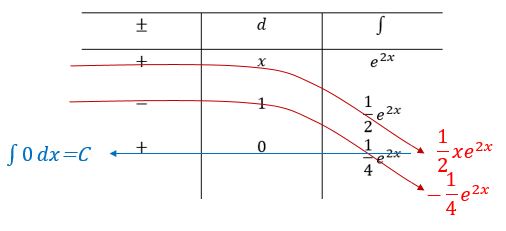
\includegraphics[scale=0.9]{tabular9.PNG}} \end{center}
 This yields $\frac{1}{2} x e^{2x} - \frac{1}{4} e^{2x}+C$ and the result of the integration is:
$$-e^{-y} = \frac{1}{2} x e^{2x} - \frac{1}{4} e^{2x}+C$$
Solving this for $y$ gives us:
$$y = - \ln {(-\frac{1}{2} x e^{2x} + \frac{1}{4} e^{2x}-C)}$$


\begin{ex}
	$$x(x+1)(x+2) y' = (3x-3) y^2 $$
\end{ex}
Solution)
$$x(x+1)(x+2) \frac{dy}{dx} = (3x-3) y^2 $$
Divide both sides by $x(x+1)(x+2)$ and also by $y^2$ to get:
$$ \frac{1}{y^2 } dy = \frac{3x-3}{x(x+1)(x+2)} dx $$
Now we have to integrate both sides. The left side is simply:
$$\int \frac{1}{y^2 } dy = \int y^{-2} dy = - y^{-1}$$
However, the right side requires something called partial fraction expansion:
$$\frac{3x-3}{x(x+1)(x+2)} = \frac{A}{x}+ \frac{B}{x+1}+ \frac{C}{x+2}$$
We have to find $A$, $B$ and $C$ that satisfies this algebraic identity and then proceed to integrate. To do this, we multiply $x(x+1)(x+2)$ both sides to get:
$$3x-3 = A(x+1)(x+2)+ Bx(x+2)+ Cx(x+1)$$
What we have above is an \textit{algebraic identity}, which means that the above equation has to hold for all values of $x$. So whatever value we make $x$ to equal to, the equation should hold, e.g. $x=0$:
$$3(0)-3=A(0+1)(0+2)+ B\cdot 0(0+2)+ C\cdot 0(0+1)$$
$$-3 = 2A+0+0$$
$$A=-\frac{3}{2}$$
Then for $x=-1$:
$$3(-1)-3 = A(-1+1)(-1+2)+ B(-1)(-1+2)+ C(-1)(-1+1)$$
$$-6 = 0-B+0$$
$$B=6$$
Then for $x=-2$:
$$3(-2)-3 = A(-2+1)(-2+2)+ B(-2)(-2+2)+ C(-2)(-2+1)$$
$$-9 = 0+0+2C$$
$$C= -\frac{9}{2}$$
Using these values for $A$, $B$ and $C$, we have an algebraic identity
$$\frac{3x-3}{x(x+1)(x+2)} = \frac{-\frac{3}{2}}{x}+ \frac{6}{x+1}+ \frac{-\frac{9}{2}}{x+2}$$
Thus integrating the left side is same as integrating the right side:
$$\int \frac{3x-3}{x(x+1)(x+2)} dx = \int \frac{-\frac{3}{2}}{x}+ \frac{6}{x+1}+ \frac{-\frac{9}{2}}{x+2} dx $$
$$=  -\frac{3}{2} \ln{|x|} + 6 \ln{|x+1|}-\frac{9}{2}\ln{|x+2|}+C$$
So we have:
$$- y^{-1} = -\frac{3}{2} \ln{|x|} + 6 \ln{|x+1|} -\frac{9}{2}\ln{|x+2|} + C $$
Solving this for $y$, we get:
$$y = \frac{1}{\frac{3}{2} \ln{|x|} - 6 \ln{|x+1|} +\frac{9}{2}\ln{|x+2|}-C}$$

\subsection*{General and Specific Solutions }

\begin{ex} Show that $y= C e^{\frac{1}{2} x^2}$ is a solution to the differential equation $y'-xy=0$.
\end{ex}

Solution) $y'= \left( C e^{\frac{1}{2} x^2}\right)' =  C e^{\frac{1}{2} x^2}\cdot x $
Hence,
$$y'-xy= C e^{\frac{1}{2} x^2}\cdot x - x \cdot C e^{\frac{1}{2} x^2}= 0$$

In the above, the solution $y= C e^{\frac{1}{2} x^2}$ is called the \textit{general solution} of the differential equation $y'-xy=0$. It means that any function that satisfies $y'-xy=0$ can be written as $y= C e^{\frac{1}{2} x^2}$ for some value of $C$.

Suppose instead we had a initial value problem:
$$y'-xy=0, y(0)=3$$
Then the initial condition $y(0)=3$ leads to $y(0)= C e^{\frac{1}{2} 0^2} = C\cdot 1 = C =3$. Hence the answer to the initial value problem is $y= 3 e^{\frac{1}{2} x^2}$. Such an answer is called a \textit{specific solution}, because it has a specified value for the parameter $C$.

\subsection*{Newton's Law of Cooling }
Newton's law of cooling states that the rate of the change of the temperature of an object in a room is proportional to the difference between the temperature of the object and the ambient temperature, i.e.
$$\frac{dT}{dt} = k (A-T)$$

\begin{ex} A frozen pizza, initially at $32^{\circ} F $ is put into an oven that is pre-heated to $400^{\circ} F$. The pizza warmed up to $50^{\circ} F$ in 2 minutes. How long would it take to reach $200^{\circ} F$ ?
\end{ex}
Solution)
Since the ambient temperature is $400^{\circ} F$, the Newton's equation becomes:
$$\frac{dT}{dt} = k (400-T)$$
Divide by $(400-T)$ and integrate:
$$\int \frac{1}{400-T} dT = \int k dt$$
$$-\ln(400-T) = kt + C $$
Solving for $T$ gives us:
$$T=400-e^{-kt-C}$$
Now, using the trick of introducing $\tilde{C}$ and then erasing the tilde, we can write:
$$T=400-C e^{-kt}$$
Now, we apply the two conditions:
a) Initial temperature was 32 : $T(0)=32$
b) Temperature became 50 in 2 minutes : $T(2)= 50$.
$T(0)=32$ implies that
$$32 = 400 - C e^{0}$$
$$C=400-32=368$$
Then $T(2)=50$ implies that
$$50= 400 - 368 e^{-2k}$$
Solving for $k$, we get:
$$k= -\frac{1}{2} \ln{\frac{350}{368}} = 0.02507$$
Thus the temperature at time $t$ is:
$$T(t) = 400- 368 e^{-0.02507t}$$
So in order to reach $200^{\circ} F$, we have to solve:
$$200 = 400- 368 e^{-0.02507t}$$
Solving this for $t$ gives us 24.3 minutes.



\subsection*{A separable differential equation that is first order linear }
In the next section, you will learn something called 'First order linear differential equation' and then if you see the following example again you will realize that this is an example of such an equation. So you can solve this differential equation using the method you will learn in the next section. So we will revisit this example in the next section. 

\begin{ex}
	$$(x^2+4) y' = 3xy$$
\end{ex}
Solution)

$$(x^2+4) \frac{dy}{dx} = 3xy$$
$$ \frac{1}{y} dy = \frac{3x}{x^2+4} dx $$
$$ \int \frac{1}{y} dy = \int \frac{3x}{x^2+4} dx $$
$$ \ln y = \frac{3}{2} \ln{(x^2+4)} +C $$
$$y = e^{\frac{3}{2} \ln{(x^2+4)} +C}$$
$$y = \tilde{C} e^{\ln{(x^2+4)^{3/2}}}$$
$$y = \tilde{C} (x^2+4)^{3/2}$$
So the answer is
$$y = C (x^2+4)^{3/2}$$

\section{First Order Differential Equations}
\subsection*{ Introduction to first order linear differential equations}
Suppose we have an equation, say,
$$x^2 y = e^{3x}$$
Now, try differentiating the above using \textit{implicit differentiation} (hopefully you still remember how to do implicit differentiation).
$$\left( x^2 y \right)' = \left( e^{3x} \right)'$$
The right side is just a regular chain rule, which yields $ 3 e^{3x} $. However, when you differentiate the left side, you have to know that $y$ is actually $y(x)$, i.e. it is a function of $x$. So when you differentiate $\left( x^2 y \right)'$, think of differentiating $\left( x^2 f(x) \right)'$, which means you have to differentiate using the product rule:
$$\left( x^2 y \right)'= \left( x^2 \right)' y  +  x^2 \left( y \right)' = 2xy + x^2 y' $$
Thus the derivative of $x^2 y = e^{3x}$ is
$$ 2xy + x^2 y'= 3 e^{3x} $$
Please look at the above equation again. Isn't it a differential equation? Yes! Now, what's the solution to the above differential equation? Well, since it came from $x^2 y = e^{3x}$, all we have to do is trace it back, i.e. do the reverse process of what we did when we differentiated it by implicit differentiation.

Before we start thinking about the way back to the answer, we will further change the differential equation $ 2xy + x^2 y'= 3 e^{3x} $ by dividing it by the coefficient of $y'$ - which in our case is $x^2$ both sides -into something called the standard form as follows:
$$ \frac{2x}{x^2} y + \frac{x^2}{x^2} y'= \frac{3 e^{3x}}{x^2} $$
$$ \frac{2}{x} y + y'= \frac{3 e^{3x}}{x^2} $$
Then switching two terms on the left:
$$  y'+ \frac{2}{x} y = \frac{3 e^{3x}}{x^2} $$
The above has the form $y'+p(x) y = q(x)$

\begin{df}
If a differential equation satifies the following properties, we call it a \textbf{first order linear differential equation\index{first order linear differential equation}}.
\begin{itemize}
\item All appearances of $y$ and $y'$ have power of 1  
\item $y$ and $y'$ are not multiplied together 
\item $y$ and $y'$ are not nested inside a function such as cos, sin, exp, square roots ... etc.
\end{itemize}
\end{df}

In general, a linear differential equation of any order is the above property holding for any order derivative of $y$.

\begin{df}
Any first order linear differential equation can be put into the form
$$y'+p(x) y = q(x)$$
This is called the \textbf{standard form\index{standard form, of first order linear DE }} of a first order differential equation.
\end{df}

Now, let's trace back what we have done to solve the following problem:
\begin{ex} Solve
$$  y'+ \frac{2}{x} y = \frac{3 e^{3x}}{x^2} $$
\end{ex}
Solution) We multiply $x^2$ both sides (this function is called the \textit{multiplier} because it is multiplied to both sides. We know we should multiply $x^2$ because we have divided by it in order to arrive at our question. Remember, we are reverse-engineering.)
$$ 2xy + x^2 y'= 3 e^{3x} $$
Now, notice that the left side is same as $\left( x^2 y \right)'$, if we apply the \textit{product rule} to $\left( x^2 y \right)'$, we get $ 2xy + x^2 y'$  (Again, we know this because we are reverse-engineering.) So we can write:
$$ \left( x^2 y \right)'= 3 e^{3x} $$
Integrate both sides:
$$ \int \left( x^2 y \right)' dx = \int 3 e^{3x} dx $$
Notice that on the left side, the integral and the derivative will cancel each other. So we have:
$$ x^2 y  = \int 3 e^{3x} dx $$
After calculating the integral on the right side, we have:
$$ x^2 y  =  e^{3x} + C $$
Finally, we solve for $y$ to arrive at our answer:
$$ y  =  \frac{1}{x^2} e^{3x} + \frac{C}{x^2}  $$

Note: Let's look at the solution and think about how it would be possible to solve such an equation if we hadn't worked out the implicit differentiation before. Two things stand out. First is "how can we figure out the multiplier?". Second is "How do we recognize the product rule?" We will address this question in the next example.

\subsection*{ The Multiplier for the First Order Linear Differential Equation}

Let's say we are given a first order differential equation in the standard form:
$$y'+p(x) y = q(x)$$

The aim of this section is to find the multiplier $M(x)$ that we can multiply on both sides of the above equation so that the left side turns into a product rule form, i.e.
$$M(x) y'+ M(x)p(x) y = M(x)q(x)$$
such that the left side $M(x) y'+ M(x)p(x) y$ is equal to $\left( M(x) y \right)' $. What does this requirement mean? Well, first try to work out the product rule:
$$\left( M(x) y \right)' = M'(x) y + M(x) y' = M(x) y' + M'(x) y$$
If we compare this with $M(x) y'+ M(x)p(x) y$, we realize that what we want is $M(x) p(x) = M'(x)$. If this is true, then we do have $M(x) y'+ M(x)p(x) y =  M(x) y' + M'(x) y = \left( M(x) y \right)'$ and the left side of $M(x) y'+ M(x)p(x) y = M(x)q(x)$ does become a product rule form.
Let's try to figure out what $M(x)$ should be:
$$M(x) p(x) = M'(x)$$
$$M p(x) = \frac{dM}{dx}$$
$$ p(x) dx = \frac{1}{M} dM $$
$$ \int p(x) dx = \int \frac{1}{M} dM $$
$$ \int p(x) dx = \ln M + C $$
Now, the above suggests that there are many different possible $M(x)$, because each time we choose a different $C$ we will have a different $M(x)$. However, we are only looking for one such function. So let's set $C=0$ and move on:
$$ \int p(x) dx = \ln M $$
$$ e^{\ln M} = e^{\int p(x) dx} $$
$$M(x) = e^{\int p(x) dx} $$
So we have obtained an important result:
\begin{df} \textbf{Multiplier.\index{multiplier for first order linear DE}}
To solve $y'+p(x) y = q(x)$, one has to compute $M(x) = e^{\int p(x) dx} $ and multiply it to both sides. The result will be that the left side becomes same as $\left( M(x) y \right)'$
\end{df}

\begin{ex}
$$y'+2y=x$$
\end{ex}
Solution) Since $p(x)=2$,
$$M(x) = e^{\int 2 dx} = e^{2x}$$
(Notice that we did not put $C$ when we integrated, because we only need one such function.)
Multiply this both sides:
$$e^{2x}y'+2e^{2x}y=xe^{2x}$$
This turns the left side into a product rule:
$\left(e^{2x}y \right)'=xe^{2x}$
So we integrate:
$$e^{2x}y = \int xe^{2x} dx$$
(Notice that the derivative on the left side disappeared because it cancelled with the integral.)
The integral on the right can be computed using tabular integration as follows:
\begin{center} \makebox[\textwidth]{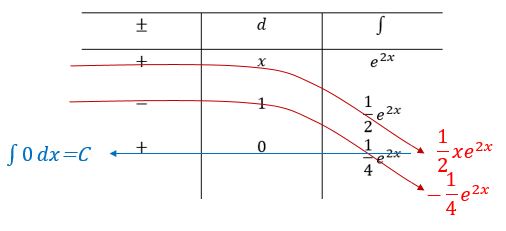
\includegraphics[scale=0.9]{tabular9.PNG}} \end{center}
(See appendix for the explanation of tabular integration.) Then we have:
$$e^{2x}y = \frac{1}{2} x e^{2x} - \frac{1}{4} e^{2x}+C$$
and solving for $y$ gives us the answer:
$$y = \frac{1}{2} x  - \frac{1}{4} +C e^{-2x}$$


\subsection*{ Examples of first order linear differential equation }
\begin{ex} Solve
$$y' - 2xy = 3x,  \; y(0)=1$$
\end{ex}
Solution)
Since $p(x)=-2x$ (Note: must include the negative sign if there is one!),
$$M(x) = e^{\int (-2x) dx} = e^{-x^2}$$
Multiplying this both sides:
$$e^{-x^2}y' - 2xe^{-x^2} y = 3xe^{-x^2}$$
$$\left( e^{-x^2} y \right)' = 3xe^{-x^2}$$
$$ e^{-x^2} y  = \int 3xe^{-x^2} dx $$
Setting $u=-x^2$, $du=-2x dx$ which leads to $dx = -\frac{1}{2x} du$. Thus
$$\int 3xe^{-x^2} dx = \int 3x e^u \left(-\frac{1}{2x}\right) du$$
$$= \int -\frac{3}{2} e^u du = -\frac{3}{2} e^u+C = -\frac{3}{2} e^{-x^2}+C$$
Using this result, we have:
$$ e^{-x^2} y  =-\frac{3}{2} e^{-x^2}+C $$
Solving for $y$, we get the general solution:
$$ y = -\frac{3}{2}+ C e^{x^2} $$
To get the specific solution satisfying $y(0)=1$, we solve:
$$1= -\frac{3}{2}+ C e^{0^2}$$
$$C= 1+\frac{3}{2}=\frac{5}{2}$$
Answer:
$$y = -\frac{3}{2}+ \frac{5}{2} e^{x^2} $$

\begin{ex} Solve
$$2xy' = y+ 3\sqrt{x^5} $$
\end{ex}
Solution) Since we see that $y'$ has power of 1 and also $y$ has power of 1, we know that this is a first order linear differential equation. We solve it using the following steps:

\textbf{Step 1} Change to standard form
Divide by the coefficient of $y'$, which is $2x$:
$$y'= \frac{1}{2x} y + \frac{3 x^{5/2}}{2x} $$
Then make it into $y'+p(x) y = q(x)$ form by moving terms:
$$y'- \frac{1}{2x} y = \frac{3 x^{5/2}}{2x} $$

\textbf{Step 2} Identify the function $p(x)$ and compute $M(x)$
Since $- \frac{1}{2x}$ is in front of $y$ in the standard form, that is our $p(x)$. \textit{Make sure you include the negative sign if there is one.} Then
$$M(x) = e^{\int -\frac{1}{2x} dx} = e^{-\frac{1}{2} \int \frac{1}{x} dx}$$
$$= e^{-\frac{1}{2} \ln x } = e^{\ln x^{-1/2}} = x^{-1/2}$$
In the above calculation \textit{study carefully how the expression was simplified. } You must simplify $M(x)$ in order to use it. (If you don't you'll run into very complicated integrals.) Remember, $e$ and $\ln$ only cancel if they are directly next to each other. That's why I had to move the $-\frac{1}{2}$ away before cancelling the two.

\textbf{Step 3} Multiply the $M(x)$ to the \textit{standard form} and make the left side into a product rule form
I want to stress again that $M(x)$ \textit{should be multiplied to the standard form, not the original given differential equation.} Thus:
$$ x^{-1/2}y'- x^{-1/2}\frac{1}{2x} y = x^{-1/2}\frac{3 x^{5/2}}{2x} $$
$$ \left(x^{-1/2}y\right)' = x^{-1/2}\frac{3 x^{5/2}}{2x} $$
Ideally, you would check that the two equations written above are indeed the same thing by applying the product rule to the bottom equation, but as you become more confident in solving differential equations this way, you can just write the above form by faith. You also have to \textbf{simplify the right side. }
$$x^{-1/2}\frac{3 x^{5/2}}{2x} = \frac{3}{2}\cdot \frac{x^{-1/2} x^{5/2}}{x}= \frac{3}{2}\cdot \frac{x^{4/2}}{x}=\frac{3}{2}x$$
Thus the differential equation is now written as:
$$ \left(x^{-1/2}y\right)' = \frac{3}{2}x$$

\textbf{Step 4} Integrate both sides and solve for $y$
$$ x^{-1/2}y = \int \frac{3}{2}x dx = \frac{3}{4}x^2 +C $$
$$ y = \frac{3}{4}x^{5/2} +C x^{1/2} $$

\begin{ex}
$$ xy'-5y = 2x, \; y(1)=0$$
\end{ex}
We will follow the steps explained in the previous example.
$$ y'-\frac{5}{x} y = 2 $$
$$M(x) = e^ {\int -\frac{5}{x} dx} = e^{-5 \ln x} = e^{\ln x^{-5}}=x^{-5}$$
$$ x^{-5}y'-x^{-5}\frac{5}{x} y = 2x^{-5} $$
$$ \left(x^{-5}y\right)' = 2x^{-5} $$
$$ x^{-5}y = \int 2x^{-5} dx $$
$$ x^{-5}y = -\frac{1}{2} x^{-4} +C $$
$$ y = -\frac{1}{2} x +Cx^{5}$$
Now, we apply $y(1)=0$
$$ 0=y(1) = -\frac{1}{2} \cdot 1 +C (1)^{5}= -\frac{1}{2}+C$$
$$C = \frac{1}{2}$$
Answer:
$$ y = -\frac{1}{2} x + \frac{1}{2} x^{5}$$

\subsection*{First Order Linear Differential Equation involving integral of a rational function}
$$(x^2+1) \frac{dy}{dx} + 3xy = 6x $$
$$ \frac{dy}{dx} + \frac{3x}{x^2+1} y = \frac{6x}{x^2+1} $$
$$M(x) = e^{\int \frac{3x}{x^2+1} dx} $$
When doing the above integral, a handy formula to know is the following:
$$\int \frac{f'(x)}{f(x)} dx = \ln f(x) +C $$
Here is how the above formula can be applied:
$$\int \frac{3x}{x^2+1} dx = \frac{3}{2}\int \frac{2x}{x^2+1} dx = \frac{3}{2} \ln {(x^2+1)} +C $$
(Notice how 3 was pulled out of the integral and also 2 was introduced. All this was necessary so that the integrand has the form of $\frac{f'(x)}{f(x)} $.)
Therefore,
$$M(x) = e^{\int \frac{3x}{x^2+1} dx} = e^{\frac{3}{2} \ln {(x^2+1)}}$$
$$ = e^{\ln {(x^2+1)^{3/2}}} = (x^2+1)^{3/2}$$
Note that we don't include $C$ when computing $M(x)$. Now multiply the multiplier to the standard form:
$$ (x^2+1)^{3/2}\frac{dy}{dx} + (x^2+1)^{3/2}\frac{3x}{x^2+1} y = (x^2+1)^{3/2}\frac{6x}{x^2+1} $$
$$ \left((x^2+1)^{3/2}y \right)'= (x^2+1)^{3/2}\frac{6x}{(x^2+1)^1} $$
$$ \left((x^2+1)^{3/2}y \right)'= (x^2+1)^{1/2}\cdot 6x $$
$$ (x^2+1)^{3/2}y = \int (x^2+1)^{1/2}\cdot 6x dx $$
Using $u=x^2+1$, we get:
$$\int (x^2+1)^{1/2}\cdot 6x dx =3\int u^{1/2} du = 2 u^{3/2} +C = 2(x^2+1)^{3/2}+C$$
So we have:
$$ (x^2+1)^{3/2}y = 2(x^2+1)^{3/2}+C $$
Answer is:
$$y = \frac{2(x^2+1)^{3/2}+C}{x^2+1} = 2(x^2+1)^{1/2}+\frac{C}{x^2+1}$$

\subsection*{First Order Linear Differential Equation involving u substitution and integration by parts}
\begin{ex}
$$ x^2 y' + y = \frac{1}{x}, \; y(1)=0 $$
\end{ex}
Solution)
$$ y' + \frac{1}{x^2} y = \frac{1}{x^3} $$
$$ M(x) = e^{\int \frac{1}{x^2} dx} = e^{-\frac{1}{x}}$$
$$ e^{-\frac{1}{x}}y' + e^{-\frac{1}{x}}\frac{1}{x^2} y = e^{-\frac{1}{x}}\frac{1}{x^3} $$
$$ \left(e^{-\frac{1}{x}}y\right)' = e^{-\frac{1}{x}}\frac{1}{x^3} $$
$$ e^{-\frac{1}{x}}y = \int e^{-\frac{1}{x}}\frac{1}{x^3} dx$$
Take $u= -\frac{1}{x}$ so that $du = \frac{1}{x^2} dx$. Solving for $dx$ we have $dx = x^2 du$. So
$$\int e^{-\frac{1}{x}}\frac{1}{x^3} dx = \int e^u \frac{1}{x^3} x^2 du = \int e^u \frac{1}{x} du= \int -e^u u du$$
This needs integration by parts, or tabular integration.
$$\int -e^u u du = -e^u u + e^u +C =(1-u)e^u +C = (1+\frac{1}{x})e^{-\frac{1}{x}}+C$$
Thus we have:
$$ e^{-\frac{1}{x}}y = \left(1+\frac{1}{x}\right)e^{-\frac{1}{x}}+C$$
Now, the general solution is:
$$ y = 1+\frac{1}{x}+ C e^{\frac{1}{x}} $$
To satisfy $y(1)=0 $,
$$0 = y(1) = 1+\frac{1}{1}+ C e^{\frac{1}{1}}=2+ eC$$
$$C=-\frac{2}{e}$$
So the answer is:
$$ y = 1+\frac{1}{x}+ -\frac{2}{e} e^{\frac{1}{x}} $$

\section{Exact Differential Equations}

\subsection*{Introduction to Exact Differential Equations}

Let's start with an example problem:
\begin{ex}
$$x^2 y +5xy^2 +3y^3 =0 $$
Find $y'$ using implicit differentiation.
\end{ex}
Solution)
$$\left(x^2 y\right)' +\left(5xy^2\right)' +\left(3y^3\right)' =0 $$
$$x^2 y' +2xy + 10xy y' + 5y^2 + 9y^2 y' =0 $$
 After this, one has to solve the above equation for $y'$ to get the answer. Now, let's try to look at this a bit differently than what you were taught in Calculus I.


\subsection*{Using Multivariable Chain Rule for Implicit Differentiation }
In Calculus III (Multivariable Calculus), you learned something called multivariable chain rule. Using that, one can come up with a fantastically easy way to solve implicit differentiation problems.
Implicit differentiation questions can be seen as differentiating an equation of the form:
$$F(x,y)=0$$
In our example above, it was $x^2 y +5xy^2 +3y^3 =0 $, and the left side can be seen as $F(x,y)$. Now, although $F(x,y)$ is a function of $x$ and $y$, to differentiate implicitly is to treat $y$ as implicitly being a function of $x$. In other words, the function $F$, and variables $y$ and $x$ have the following dependence:
\begin{center}
	\makebox[\textwidth]{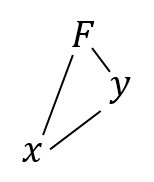
\includegraphics[scale=0.5]{depdiag1.PNG}}
\end{center}

A line drawn from $F$ to $x$ means $F$ is a quantity that changes when $x$ is changed. Other lines can be interpreted similarly. Such dependence diagram leads to a chain rule of the form:
$$\frac{dF}{dx} = \frac{\partial F}{\partial x} + \frac{\partial F}{\partial y} \frac{dy}{dx}$$
You should read this chain rule as "The rate of change of $F$ when you change $x$ is the sum of two things. First is the rate of change of $F$ when $x$ is changed but $y$ is fixed. Second is the rate of change of $F$ when change of $x$ gives rise to change in $y$ which in turn changes $F$." If you see the dependence diagram again, there are two 'routes' from $x$ to $F$: one going directly and another going through $y$. The two terms in $\frac{\partial F}{\partial x} + \frac{\partial F}{\partial y} \frac{dy}{dx}$ measures the change in $F$ brought about by change of $x$ going through each of the two 'routes'. The magic of the multivariable chain rule is that if you add these up, you can find the total rate of change of $F$ brought about by change of $x$.
What does this have anything to do with the implicit differentiation? Well, differentiating both sides $F(x,y)=0$ by $x$ is:
$$\frac{\partial F}{\partial x} + \frac{\partial F}{\partial y} \frac{dy}{dx} =0 $$
where the left side is the chain rule. Let's rewrite this equation using slightly different notation. First we use $F_x$ for $\frac{\partial F}{\partial x}$, and also likewise $F_y$. Then instead of $\frac{dy}{dx}$ we use $y'$. The equation now reads:
$$F_x + F_y y'=0$$
Now, since we are looking for $y'$, all we have to do is to solve for $y'$.
$$ F_y y'= - F_x$$
$$ y' = - \frac{F_x}{F_y} $$

\subsection*{Awesomely easy formula for solving implicit differentiation problems }
So we have the following result: If an implicit differentiation problem is given in the form of
$$F(x,y)=0,$$
The answer is $ y' = - \frac{F_x}{F_y} $

If you use the above formula for $x^2 y +5xy^2 +3y^3 =0 $, you will recognize that this formula indeed works. (You may even want to take Calculus I again so you can ace that test on implicit differential equation!) However, since we are not here to solve implicit differentiation questions, but differential equations, we will only make use of the following fact:
$$F(x,y)=0 \; \; \; \rightarrow \; \; \; F_x + F_y y'=0$$

How does the above fact solve differential equation? Here is an example problem:
\begin{ex} Solve
$$x^2 y' +2xy + 10xy y' + 5y^2 + 9y^2 y' =0 $$
\end{ex}
Solution)
First, gather all the terms that have $y'$ attached and factor the $y'$ from them to get:
$$ 2xy + 5y^2 + (x^2 +10xy + 9y^2) y' =0 $$
Now what we aim to do is to find out what it was before the differentiation. In other words, we are imagining the original equation as an equation of the form $F(x,y)=0$ and then implicit differentiation was applied to get the above equation. Since the derivative of $F(x,y)=0$ is $F_x + F_y y'=0$, comparing this with the above equation reveals that:
$$F_x = 2xy + 5y^2 $$
$$F_y = (x^2 +10xy + 9y^2)$$
Integrating $F_x = 2xy + 5y^2 $ by $x$ yields:
$$F = \int 2xy + 5y^2 dx = x^2 y + 5y^2 x + g(y)$$
Notice that instead of $C$, I wrote $g(y)$. The reason for this is that since partial derivative $F_x$ computed by regarding $y$ as a constant, the things that get deleted by derivatives could have been a function of $y$.
For similar reasons, if we integrate $F_y = (x^2 +10xy + 9y^2)$ we will need to put a function of $x$:
$$F = \int  (x^2 +10xy + 9y^2) dy = x^2 y + 5 x y^2 + 3 y^3 + h(x)$$
Now, this is similar to figuring out the details of an unknown object (in this case $F(x,y)$) from two different reports (the two integral results we see above.) To get a clear picture, we have to harmonize the two different accounts of $F(x,y)$. If you compare them, you can see that indeed the two descriptions do agree that $F(x,y)$ must contain $x^2 y + 5 x y^2$. Also, you see that what we called $g(y)$ in the first integral must be same as $3 y^3$, while $h(x)$ must be zero. This investigation can conclude what $F(x,y)$ is up to a constant, i.e.
$$F(x,y) = x^2 y + 5 x y^2 + 3 y^3 + C$$
(If you studied hard in multivariable calculus, you will recognize this method as finding the potential function of a conservative vector field problem.) Now that we found the $F(x,y)$, we can claim that the original equation before differentiation is
$$x^2 y + 5 x y^2 + 3 y^3 + C = 0$$
To verify that indeed this equation is correct, just do implicit differentiation. WAIT! Didn't we do that in the beginning? Yes. Go back and check that this is indeed what we started with (except for that $C$, which appears as the result of integration.)
This somewhat convoluted approach is just a way to say that solving exact differential equation is basically undoing the implicit differentiation. I have not defined what exact differential equation is yet. It will be given in the next section.

\subsection*{Yet another introduction to Exact differential equations}
$$ (2xy) dx + (x^2 - 4y) dy =0$$
This is an example of an \textit{exact differential equation}. However, we haven't defined what exact differential equation is. That will be given after the solution of this problem.
A little note about the strange looking symbols $dx$ and $dy$:  If you divide both sides by $dx$, you get:
$$ (2xy) + (x^2 - 4y) \frac{dy}{dx} =0$$
This looks more natural because $\frac{dy}{dx}$ has the meaning of the derivative of $y$, where as $dx$ and $dy$ we had before is hard to understand. (Some calculus courses teach $dx$ and $dy$ as differentials.)
However, many differential equation textbooks present problems in the form of $ (2xy) dx + (x^2 - 4y) dy =0$, because in this form, it is easier to recognize whether the given differential equation is exact.

To understand how to solve this equation, we need to review the multivariable chain rule for the following dependence diagram:

\begin{center}
	\makebox[\textwidth]{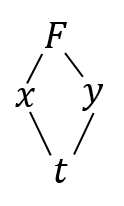
\includegraphics[scale=0.5]{depdiag2.PNG}}
\end{center}

In other words, we have a function $F(x,y)$ and both $x$ and $y$ are functions of $t$.
The chain rule associated with the dependence diagram above is:
$$\frac{dF}{dt}=\frac{\partial F}{\partial x}\frac{dx}{dt} + \frac{\partial F}{\partial y} \frac{dy}{dt} $$
If we multiply $dt$ both sides, we get
$$ dF = F_x dx + F_y dy$$
This is called the \textit{total derivative} of $F$.

What we want to do is to look at our problem $ (2xy) dx + (x^2 - 4y) dy =0$ and understand it as $dF =0$ for some function $F(x,y)$. If that is done, then we can integrate $dF =0$ both sides to get $F(x,y) =C$ as the answer to the exact differential equation. If such $F(x,y)$ do exist, then comparing $dF = F_x dx + F_y dy$ with $ (2xy) dx + (x^2 - 4y) dy =0$, we can conclude that $F_x = 2xy$ and $F_y = (x^2-4y)$. Using that we can figure out $F(x,y)$. But it turns out that this is not always possible. For such $F(x,y)$ to exist, we some condition to be met, explained in the next section.

\subsection*{Checking if a given differential equation is exact }
It is one of the basic fact that you learn in multivariable calculus that the partial derivatives commute, i.e.
$$F_{xy} = F_{yx}$$
In other words, if you take a function and differentiate it by $x$ first and then $y$, you will get the same answer as if you differentiated by $y$ first and then $x$. Since we are claiming that $F_x = 2xy$ and $F_y = (x^2-4y)$ in our question, we need to verify whether $F_{xy} = F_{yx}$ does hold true or not.
Now, $F_{xy} = \partial_y F_x = \partial_y (2xy) = 2x $. Also, $F_{yx} = \partial_x F_y = \partial_x (x^2-4y) = 2x$. So we find that indeed $F_{xy} = F_{yx}$ does hold. What is surprising is that mathematician Henry Poincare proved that this is the only condition one needs to verify in order to find out whether $F(x,y)$ exists or not. (Actually, there are some more delicate conditions in addition to this, but we will never have to deal with other conditions.) Here is the statement:

\subsection*{Test for exactness}
Suppose a differential equation is given as
$$P(x,y) dx + Q(x,y) dy =0$$
Then if $P_y = Q_x$, we say that the differential equation is \textbf{exact\index{exact}}, or that the above is an \textbf{exact differential equation\index{exact differential equation}}.

Once we verify that the differential equation is exact, then just remembering that $F_x$ is the one in front of $dx$ and $F_y$ is in front of $dy$ will guide us to find $F(x,y)$. In our example,
$$F_x = 2xy \; \; \; \rightarrow \; \; \; F= \int 2xy dx = x^2y +g(y)$$
$$F_y = (x^2-4y)\; \; \; \rightarrow \; \; \; F= \int (x^2-4y) dy = x^2 y -2y^2 + h(x)$$
Comparing the two, we conclude that:
$$F(x,y) = x^2 y - 2y^2$$
and the answer to $ (2xy) dx + (x^2 - 4y) dy =0$ is:
$$x^2 y - 2y^2 = C$$
\textit{PLEASE DON'T FORGET THE C!}

\subsection*{Exact Differential Equations example. }
\begin{ex}
Verify the following D.E. for exactness and solve:
$$(3x \cos y + 5) dx + \left(-\frac{3}{2} x^2 \sin y + 3y^2\right) dy = 0$$
\end{ex}
Solution)
\textit{Step 1.} Check for exactness.
The formula $dF= F_x dx + F_y dy$ tells us that $F_x = (3x \cos y + 5) $ and $F_y = (-\frac{3}{2} x^2 \sin y + 3y^2)$. We have to check whether $F_{xy} = F_{yx}$ holds or not.
$$F_{xy} = \partial_y F_x = \partial_y (3x \cos y + 5)  = -3x \sin y $$
$$F_{yx} = \partial_x F_y = \partial_x \left(-\frac{3}{2} x^2 \sin y + 3y^2\right) = -3x \sin y $$
Thus we see that it is exact.
\textit{Step 2.} Integrate and figure out $F(x,y)$
$$F_x = (3x \cos y + 5) \; \; \; \rightarrow \; \; \; F= \int (3x \cos y + 5) dx = \frac{3}{2} x^2 \cos y + 5x +g(y)$$
$$F_y = \left(-\frac{3}{2} x^2 \sin y + 3y^2\right)\; \; \; \rightarrow \; \; \; F= \int \left(-\frac{3}{2} x^2 \sin y + 3y^2\right) dy = \frac{3}{2} x^2 \cos y + y^3+ h(x)$$
Comparing the two, we conclude that $g(y)=y^3$ and $h(x)=5x$ which means:
$$F = \frac{3}{2} x^2 \cos y + y^3+ 5x $$
\textit{Step 3.} Set the function equal to $C$
The answer is :
$$\frac{3}{2} x^2 \cos y + y^3+ 5x =C $$

\subsection*{An equation which is both exact and first order linear}
So far we have learned three types of differential equations: Separable, First order linear and Exact. Here is an example of a question which is both first order linear and exact.
\begin{ex}
$$5x^2 +2y + 2xy' = 0$$
\end{ex}
\textit{Solution 1)} We solve this thinking of it as a first order linear differential equation:
$$ y' + \frac{1}{x} y = -\frac{5}{2} x $$
$$M(x) = e^{\int \frac{1}{x} dx} = e^{\ln x } = x$$
$$ x y' + x \frac{1}{x} y = -x \frac{5}{2} x $$
$$ xy' + y = -\frac{5}{2} x^2 $$
$$ (xy)' = -\frac{5}{2} x^2 $$
$$ xy = \int -\frac{5}{2} x^2 dx = -\frac{5}{6} x^3+ C$$
$$ y = -\frac{5}{6} x^2 + \frac{C}{x}$$
\textit{Solution 2)} We solve this by thinking of it as an exact differential equation.
First, rewrite $y' = \frac{dy}{dx}$ and multiply $dx$ to get:
$$(5x^2+2y)dx + 2x dy =0$$
Then $\partial_dy  (5x^2+2y) = 2$ and $\partial_x 2x = 2$. Therefore this differential equation is exact.
This means that there is a function $F(x,y)$ which satisfies $F_x = (5x^2+2y)$ and $F_y = 2x $.
$$F_x = (5x^2+2y) \; \; \; \rightarrow \; \; \; F= \int (5x^2+2y) dx = \frac{5}{3} x^3 +2xy+g(y)$$
$$F_y = (2x)\; \; \; \rightarrow \; \; \; F= \int (2x) dy =  2xy + h(x)$$
Answer:
$$ 2xy + \frac{5}{3} x^3 =C $$
If you solve this for $y$, you will see that both answers are the same.

\subsection*{Exact differential equation with $(1+ e^{xy})dx$ term.}
\begin{ex}
$$(1+y e^{xy})dx +(2y+x e^{xy})dy =0$$
\end{ex}
Solution)
Checking exactness:
$$\partial_y (1+y e^{xy}) = e^{xy}+ xy e^{xy}$$
$$\partial_x (2y+x e^{xy}) = e^{xy}+ xy e^{xy}$$
Hence they match and we know that the given differential equation is exact.
$$F_x = (1+y e^{xy})\; \; \; \rightarrow \; \; \; F= \int (1+y e^{xy}) dx = x + e^{xy} + g(y) $$
$$F_y = (2y+x e^{xy})\; \; \; \rightarrow \; \; \; F= \int (2y+x e^{xy}) dy =  y^2 + e^{xy} + h(x)$$
So the answer is:
$$ x+ y^2 +e^{xy} =C$$

\chapter{Higher Order Linear Differential Equations}
\section{Independence of Solutions and Wronskians}
\subsection*{Introduction to Higher Order Linear Differential Equations}
Order of a differential equations is the highest derivative that appears in the equation. Here are some examples:\\

Second order : $y''+5xy+x^7 \cos 5x =0 $\\

Fifth order : $ 8y''+9x^2 y^{(5)} + (x+2)y=0$\\

Higher order differential equations (i.e. equations whose order is 2 or above) are much harder than first order differential equations.
Therefore, we take a different approach than what we have done for first order differential equations.

\subsection*{Solving vs. Guessing}
Let's say we have an equation  $3x-6=0$.\\
\textit{Solving} would be first adding 6 both sides to get 3x=6 and then divide by 3 to get $x=2$ as the answer.\\
\textit{Guessing} would be trying 1,2,3... for the value of x and then find out that when $x=2$, we have $3x-6=3\cdot 2-6=0$, and thus $x=2$ is the answer.
All your life you were told that guessing is bad and you should learn how to solve. However, when it comes to higher order differential equations, we will be guessing rather than solving.
To make it sound a little nicer, we will do "educated guessing" and much of the learning would be invested in what type of solution would be appropriate for the solution. We will also call this "solving" so we feel better about ourselves.

\subsection*{What justifies "guessing"?}
Thankfully, guessing the solutions of a linear differential equation is justified because mathematicians proved two important theorems about it. They are:
\begin{itemize}
	\item \textbf{Existence\index{existence of solutions}} of solutions
	\item \textbf{Uniqueness\index{uniqueness of solutions}} of the solution given appropriate initial conditions
\end{itemize}
Existence  allows you do go ahead and hunt for a solution. If we don't know whether the solution of a differential equation exists, then we may end up hunting for the solution forever. (Or wrongly think that a false solution you found is a solution)
Uniqueness allows you to say that the solution you found is the only one, and thus you don't have to find more.

\subsection*{Uniqueness further explained}
For second order linear differential equations, there is only one solution if you set values for $y(a)$ and $y'(a)$, e.g.
$$y''-6y'-7y=0, \; y(3)=-1, y'(3)=4$$ will have only one function satisfying it.
In the above, $y(3)=-1, y'(3)=4$ are called \textbf{initial conditions\index{initial condition of ODE}}.
For nth order linear differential equations, n initial conditions should be provided to have a unique solution.
Recall that when you solved a first order differential equation without an initial condition, there was always a free parameter $C$ in your solution.
Second order differential equations without a given initial condition will have two free parameters, whose values will be determined if two initial conditions are provided.

\subsection*{ Why linear independence of functions is needed}
Now let's try to guess the solution to a very simple second order linear differential equation:
$$y''=y$$
I know that $y=e^x$ is a function whose derivative is same as itself, so it would satisfy the above equation.
Then after trying many different functions, we find that $y=e^{-x}$ is another solution. (Quick check: $y'=-e^{-x}$. $y''=e^{-x}=y$.)
Whenever we find two different solutions like these, take the \textbf{linear combination\index{linear combination}} of the two functions as:
$$y= C_1 e^x + C_2 e^{-x}$$
Then you can check that this is a solution to $y''=y$. This is a good thing, because we managed to have \textit{two free parameters} for our second order differential equation, which means we have found the most general solution to this differential equation.

Note: 1. Later, we will learn what 'homogeneous' means and that linear homogeneous differential equations always have the general solution in the form of linear combination of solutions. 2. Physicists often use the word \textbf{superposition\index{superposition}} instead of \textit{linear combination}.

With the success of the first question, let's move on to a slightly harder question:
$$y''=-y$$
You may remember that $\sin x$ has second derivative that is negative of itself. So is $\cos x$. So we can quickly write down their linear combination and claim that the general solution is:
$$y= C_1 \cos x + C_2 \sin x$$
However, look at the following calculation:
$$\left(e^{ix}\right)^{''} = \left(i e^{ix}\right)^{'}=i^2 e^{ix} = -e^{ix}$$
Did you notice that $y=e^{ix}$ is also a solution to $y''=-y$?
This means that the linear combination of three functions is also a solution:
$$y= C_1 \cos x + C_2 \sin x +C_3 e^{ix}$$
But wait, this has three parameters. So something is wrong here. Thinking about the above linear combination for a while, you may come to question whether one of the functions is really other functions written in disguise. And indeed, it is true. There is something called the Euler identity, that says:
$$e^{ix}=\cos x + i \sin x$$
So really what we thought was a new solution was in fact expressible as linear combination of the other two functions. There is a language for such case. Since $e^{ix}$ was expressed as linear combination of $\sin x$ and $\cos x$, we say "$e^{ix}$ \textit{is NOT linearly independent from} $\sin x$ and $\cos x$". Still another way to say it is "$e^{ix}$ is \textbf{linearly independent\index{linearly independent}} on $\sin x$ and $\cos x$".
The upshot of this discussion is that whenever we have a set of functions that satisfy a differential equation, we should check whether those functions are \textit{linearly independent} before we make linear combination out of them to make the general solution.

\begin{df}
	Functions $f(x)$ and $g(x)$ are said to be \textbf{linearly dependent\index{linearly dependent}} if there is any pair of constants $C_1$ and $C_2$ (at least one of them non-zero) that satisfies
		$$C_1 f(x) + C_2 g(x) =0.$$
	Functions $f(x)$, $g(x)$ and $h(x)$ are said to be \textbf{linearly dependent} if there is any triple of constants $C_1$,$C_2$ and $C_3$ (at least one of them non-zero) that satisfies
		$$C_1 f(x) + C_2 g(x)+ C_3 h(x) =0.$$
\end{df}

In our previous example, the three functions $e^{ix}$, $\sin x$ and $\cos x$ are linearly dependent because
$$ 1\cdot \cos x + i\cdot \sin x + (-1)\cdot e^{ix} =0 $$
(The above is just the Euler identity written in a different way.)

Let's go back to our example in the beginning and see why linear independence is essential. Since $y''=y$ is satisfied by both $f(x)=e^x$ and $g(x)=2e^x$, can we can take their linear combination and write:
$$y = C_1 e^x + C_2 (2e^x)$$
Can this express all general solutions of $y''=y$? The answer is no because although above linear combination looks like it has two free parameters, it really has just one. To see this, notice that:
$$y = C_1 e^x + C_2 (2e^x) = (C_1 + 2C_2 )e^x$$
Since $C_1$ and $C_2$ are arbitrary, we can set $C=(C_1 + 2C_2 )$ and rewrite the above as:
$$y = C e^x$$
In other words, the linear combination only produces solutions that looks like multiples of $e^x$, and thus it really has just one free parameter.

Actually, you should have noticed even from the beginning that $f(x)=e^x$ and $g(x)=2e^x$ are linearly dependent, because one function is a multiple of the other. Since
$$g(x)=2f(x),$$
we can write it as:
$$(-2)\cdot f(x)+1\cdot g(x)=0$$
which means they are linearly dependent according to our definition.

This is true in general. "If two non-zero functions are linearly dependent, then one is the multiple of the other."

\begin{ex}
Show that $\sin x$ and $\cos x$ are linearly independent.
\end{ex}
Solution)
We will prove by contradiction. Suppose they are linearly dependent. Then one is the multiple of the other, so we can write:
$$\sin x = C \cos x$$
for some constant $C$. Now, if we divide both sides by $\cos x$, then we have :
$$\frac{\sin x}{\cos x} = C$$
$$\tan x =C $$
But this last line is a contradiction because $\tan x$ is not a constant function. Therefore, it is impossible to find such $C$ and therefore the two functions must be linearly independent.

This example shows that indeed the general solution of $y''=-y$ is $y = C_1 \cos x + C_2 \sin x$ because we have established that $\cos x$ and $\sin x$ are linearly independent of each other.

\subsection*{ Wronkian of functions }
Wronskian is a determinant introduced by Jozef Hoene-Wronski in 1776. In the previous section, we saw how cumbersome it is to prove that two functions are linearly independent. Wronskian makes it easy to determine linear independence of multiple functions.
To understand the idea behind this, let us write the condition for linear dependence, using $\sin x$ and $\cos x$:
$$C_1 \cos x + C_2 \sin x = 0$$
Now, the above is an equation of functions, which means that it is supposed to be true for \textit{any value of} $x$. Sometimes we call this (functional) identity, rather than an equation. There is a big difference between algebraic equation and functional equality. If two sides are equal as functions, their derivatives are equal to, e.g.
$$x^2 +2x+1= (x+1)^2$$
is an identity because it holds for all values of $x$. Now, if we differentiate both sides, we get:
$$2x+2 = 2(x+1)$$
where the right side was computed using the chain rule. Notice that indeed the two sides are same.
On the other hand, think about the following equation:
$$x^2 = 2x$$
This equation is only true for $x=0$ and $x=2$. So it is not an identity. In this case, the derivatives do not match:
$$2x \neq 2 $$

Since $C_1 \cos x + C_2 \sin x = 0$ is an identity, we CAN differentiate it:
$$C_1 (-\sin x) +C_2 \cos x = 0$$

So saying that $C_1 \cos x + C_2 \sin x = 0$ holds leads to the following system of equations:
$$C_1 \cos x + C_2 \sin x = 0$$
$$C_1 (-\sin x) +C_2 \cos x = 0$$
You can view this as system of equations for $C_1$ and $C_2$. Recall that you can write system of equations as matrices. In our case
$$\left( {\begin{array}{cc} \cos x & \sin x \\ -\sin x & \cos x \\ \end{array} } \right) \left( {\begin{array}{c} C_1 \\  C_2 \\ \end{array} } \right) =\left( {\begin{array}{c} 0 \\  0 \\ \end{array} } \right) $$
Such equation can be solved by multiplying the inverse matrix both sides.

$$\left( {\begin{array}{cc} \cos x & \sin x \\ -\sin x & \cos x \\ \end{array} } \right)^{-1}\left( {\begin{array}{cc} \cos x & \sin x \\ -\sin x & \cos x \\ \end{array} } \right) \left( {\begin{array}{c} C_1 \\  C_2 \\ \end{array} } \right) = \left( {\begin{array}{cc} \cos x & \sin x \\ -\sin x & \cos x \\ \end{array} } \right)^{-1} \left( {\begin{array}{c} 0 \\  0 \\ \end{array} } \right) $$
In the left side, the inverse cancels the next matrix. On the right side, any matrix multiplied by a zero matrix will produce zero matrix. Thus we have:
$$\left( {\begin{array}{c} C_1 \\  C_2 \\ \end{array} } \right) =\left( {\begin{array}{c} 0 \\  0 \\ \end{array} } \right) $$
Now this means that the only pair of constants $C_1$ and $C_2$ that satisfies $C_1 \cos x + C_2 \sin x = 0$ is $C_1=0$ and $C_2=0$. Which means that the two functions $\cos x$ and $\sin x $ are linearly independent! (Go back to the previous section and read the definition of linear dependence if you don't understand why.)
But wait, where did we use anything specific about $\cos x$ and $\sin x $ here? There is one thing I forgot to mention. Inverse matrices don't always exist. This calculation can only be possible if the matrix
$$\left( {\begin{array}{cc} \cos x & \sin x \\ -\sin x & \cos x \\ \end{array} } \right) $$
has an inverse. Recall that \textit{the inverse of a matrix exists only when the determinant is nonzero.} So in order to justify our calculation, we have to compute the determinant as follows:
$$\begin{vmatrix} \cos x & \sin x \\ -\sin x & \cos x \\ \end{vmatrix} = \cos x \cdot \cos x - \sin x \cdot (-\sin x) = \cos^2 x + \sin^2 x =1 \neq 0 $$
Since the determinant is not zero, we know that the calculations were sound and the conclusion that the two functions are linearly independent is correct.
Now, for any two functions $f(x)$ and $g(x)$, we can follow the exact same steps as above. You will find that at the end of the day, whether or not the two functions are linearly independent depends on the following determinant:
$$\begin{vmatrix} f(x) & g(x) \\ f'(x) & g'(x) \\ \end{vmatrix}$$
This matrix is called the \textbf{Wronskian\index{Wronskian}} of two functions, and is denoted as $W[ f(x); g(x) ]$. If the Wronskian is zero, then the two functions are linearly dependent, but if the Wronskian is non-zero the two functions are linearly independent. (There is some requirement about the functions being analytic, but we will avoid these technicalities.)

\subsection*{Wronskian of three functions}
The advantage of Wronskian is that it can be defined for three functions:
$$W[f(x); g(x); h(x)] = \begin{vmatrix} f(x) & g(x) & h(x) \\ f'(x) & g'(x)& h'(x) \\ f''(x) & g''(x)& h''(x) \\ \end{vmatrix}$$
Notice that this time we had to involve the second derivative too. This is because determinants are only defined for square matrices and by using the second derivative we can add one more row to the matrix to make it a $3\times3$ matrix.

Let's revisit some of the examples we investigated in the previous section:
\begin{ex}
Determine the linear dependence of $e^x$ and $2e^x$.
\end{ex}
Solution)
$$W[e^x ; 2 e^x ] = \begin{vmatrix} e^x & 2e^x  \\ e^x  & 2e^x  \\ \end{vmatrix} = e^x\cdot 2e^x - 2e^x\cdot e^x = 0$$
Thus the two functions are linearly dependent.

\begin{ex}
Determine the linear dependence of $\cos x$, $\sin x$ and $e^{ix}$.
\end{ex}
Solution)
$$W[\cos x; \sin x; e^{ix}] = \begin{vmatrix} \cos x & \sin x & e^{ix}\\ -\sin x & \cos x & ie^{ix} \\ -\cos x & -\sin x & -e^{ix} \\ \end{vmatrix}$$
We can compute this by either a row expansion or a column expansion. Let's try doing a row expansion on the second row. (Any other choice will be fine too.)
$$ = -(-\sin x) \begin{vmatrix} \sin x & e^{ix} \\ -\sin x & -e^{ix} \\ \end{vmatrix} + \cos x \begin{vmatrix} \cos x & e^{ix} \\ -\cos x & -e^{ix} \\ \end{vmatrix} - \left(-e^{ix}\right) \begin{vmatrix} \cos x & \sin x \\ -\cos x & -\sin x \\ \end{vmatrix} $$
$$ = \sin x (-\sin x e^{ix}+\sin x e^{ix}) +\cos x ( \cos x  e^{ix} - \cos x  e^{ix}) + e^{ix} ( \cos x \sin x -\cos x \sin x) =0$$
Hence the three functions are linearly dependent.

\subsection*{ Linear Operators}
An \textit{operator} is a function which takes a function as an input and gives you back another function as an output. Derivative is an example of an operator. Partial derivatives are also operators. So is a constant multiples.
A \textbf{linear operator\index{linear operator}} is an operator that satisfies the following property:
$$L( c_1 f(x) + c_2 g(x)) = c_1 L(f(x)) + c_2 L(g(x))$$
In other words, the operator $L$ has the property where it can be applied term by term and also constant multiple can be brought in front.

Here is an example of a linear operator:
$$L = D^2+5 $$
where $D$ is the operator that differentiates a function by $x$ and $5$ is the operator that multiplies by $5$. Here is how it operates on a function:
$$(D^2+5) f(x) = f''(x) + 5f(x)$$

To see that this is a linear operator, try computing:
$$(D^2+5)(c_1 f(x) + c_2 g(x)) = (c_1 f(x) + c_2 g(x))''+5(c_1 f(x) + c_2 g(x)) $$
$$= c_1 f''(x) + c_2 g''(x) + 5c_1 f(x) + 5c_2 g(x) = c_1(f''(x) + 5f(x)) + c_2(g''(x) + 5g(x))$$
$$= c_1 (D^2+5) f(x) + c_2 (D^2+5) g(x)$$

In fact, any operator that is made up of combinations of differential operator and multiplication operator will be a linear operator. For example:
$$L = 5D^2 - 6x D + (e^x -x)$$
is a linear operator. (I'll leave you to check that it is indeed true, since it's rather long.)

Why is linear operators important? It is important for us because linear differential equations always contain a linear operator in it. For example, the differential equation:
$$y'' -3y' -4y =0$$
can be written as $L y=0$ with $L=D^2 -3D -4$.

Here is a little bit more about this differential equation $y'' -3y' -4y =0$. This is a \textit{constant coefficient} second order linear differential equation. In such case, you will learn that all solutions take the form of $e^{rx}$. If we plug in $e^{rx}$ for $y$, we get:
$$\left( e^{rx} \right)'' - 3 \left(e^{rx}\right)' - 4 e^{rx} = r^2 e^{rx} -3 re^{rx}- 4e^{rx}=(r^2-3r-4)e^{rx}$$
Since $e^{rx}$ can never be zero, the only way the above can be $=0$ is when $(r^2-3r-4)=0$. Factoring this as $(r-4)(x+1)=0$, we find that $r= -1, 4$. This means that there are two solutions to this differential equation: $y=e^{-x}$ and $y=e^{4x}$. You can also compute their Wronskian and find that these two functions are linearly independent.

If we use the language of operators, $y=e^{4x}$ being the solution to $y'' -3y' -4y =0$ is same thing as saying $L\left(e^{4x}\right)=0$, with $L=D^2 -3D -4$. Likewise $L\left(e^{-x}\right)=0$. Here is \textit{why linearity is important}:
$$L\left(c_1 e^{4x} + c_2 e^{-x} \right)=c_1 L\left(e^{4x}\right)+c_2 L\left(e^{-x}\right) = c_1\cdot 0+c_2\cdot0=0 $$
Look at how the linearity of the operator was used to show that the linear combination of two functions is again a zero if $L$ is applied, i.e. $c_1 e^{4x} + c_2 e^{-x}$ is the general solution of $y'' -3y' -4y =0$

\subsection*{Conclusion}
In other words, if your differential equation can be written in a form of $L y =0$ with a linear operator $L$, then any linear combination of solutions is again a solution, due to the linear property of the operator $L$.


\section{Second Order Linear Differential Equations}
	\subsection*{Introduction to second order constant coefficient homogeneous linear differential equations}
A \textit{second order linear constant coefficient homogeneous differential equation} is a differential equation of the form:
$$a y''+by'+cy=0$$
These are the simplest forms of second order differential equations. They have the solution of the form $y=e^{rx}$. Since $y'=r e^{rx}$ and $y''=r^2 e^{rx}$, plugging this into the above differential equation yields:
$$a r^2 e^{rx} + b r e^{rx} + c e^{rx} = (a r^2 + br +c)e^{rx}$$
Since $e^{rx}$ is never zero, the only way this can be equal to zero is when:
$$a r^2 + br +c = 0$$
The above equation is called the \textbf{characteristic equation\index{characteristic equation}} of the differential equation $a y''+by'+cy=0$. Whenever we solve a differential equation of the form $a y''+by'+cy=0$, we will immediately write down the characteristic equation and solve it.
The name "characteristic equation" comes from the fact that depending on whether the quadratic equation has two distinct roots, a double root or complex roots, the solution of the differential equation takes different forms.

Let's think about the solution of $a r^2 + br +c = 0$. Using the quadratic formula:
$$r= \frac{-b \pm \sqrt{b^2-4ac}}{2a}$$
There are three different cases:
\begin{itemize}
\item  When $b^2-4ac>0$, the solutions are two real values $r_1$ and $r_2$. This means $e^{r_1 x}$ and $e^{r_2 x}$ are solutions. Then we take the linear combination of the two functions as the general solution:
	$$ y=C_1 e^{r_1 x}+ C_2 e^{r_2 x}$$
	(One should check that the two solutions are linearly independent by computing the Wronskian.)
\item  When $b^2-4ac<0$, the quadratic formula produces $r= \alpha \pm \beta i $. In this case the general solution is
$$ y=e^{\alpha x} (C_1 \cos \beta x + C_2 \sin \beta x) $$

\item  When $b^2-4ac=0$, then the quadratic formula produces just one solution $r=r_1$. Hence we only have one solution $e^{r_1 x}$. This is bad because we need two linearly independent solutions in order to write the general solution. Thankfully, someone figured out that in this case, $x e^{r_1 x}$ also becomes one solution. So the general solution is:
$$ y=C_1 e^{r_1 x}+ C_2 x e^{r_1 x}$$
\end{itemize}

\subsection*{Second order constant coefficient homogeneous linear differential equations: Two distinct real roots}

\begin{ex} Solve
$$y''-6y'+8y=0, \; y(0)=1, y'(0)=-6$$
\end{ex}
Solution) The characteristic equation is:
$$r^2 -6r +8=0$$
$$(r-4)(r-2)=0$$
$$r=4, \; 2$$
Hence the general solution is:
$$ y=C_1 e^{4 x}+ C_2 e^{2 x}$$
Now we want the specific solution that satisfies the initial condition $y(0)=1, y'(0)=-6$. Since $y' = C_1 \cdot 4 e^{4 x}+ C_2 \cdot 2 e^{2 x}$, we have:
$$-6 = y'(0) = C_1 \cdot 4 e^{4\cdot 0}+ C_2 \cdot 2 e^{2 \cdot 0} = 4C_1+ 2C_2 $$
Also:
$$1=y(0)= C_1 e^{4\cdot 0}+ C_2 e^{2 \cdot 0} = C_1+ C_2 $$
So we have a system of equations:
$$4C_1 + 2C_2 = -6$$
$$C_1 + C_2 = 1$$
Solving $C_1 + C_2 = 1$ for $C_2$ as $C_2 = 1-C_1$ and then plugging it into $4C_1 + 2C_2 = -6$, we get:
$$4C_1 + 2(1-C_1) = -6$$
$$2 C_1 + 2 = -6$$
$$C_1 = -4$$
$$C_2 = 1-(-4)=5$$
\textit{After finding the constants, put it back into the general solution:}
$$y = (-4) e^{4 x}+ 5 e^{2 x}$$

\subsection*{ Second order constant coefficient homogeneous linear differential equations: Double root}
\begin{ex} Solve
$$y''-8y'+16y=0, \; y(0)=2, y'(0)=0$$
\end{ex}
Solution) The characteristic equation is:
$$r^2 -8r +16=0$$
$$(r-4)(r-4)=0$$
$$r=4, \; 4$$
Now this is troubling because we only have one solution to use: $e^{4 x}$. The other solution, however, can be obtained by just multiplying by $x$. Hence the general solution is:
$$ y=C_1 e^{4 x}+ C_2 x e^{4 x}$$
To use the initial condition $y(0)=2, y'(0)=0$, we first differentiate the above:
$$y' = 4C_1 e^{4 x}+ 4C_2 x e^{4 x}+C_2 e^{4 x}$$
Thus
$$0 = y'(0)=4C_1+0+C_2$$
Now, from $y(0)=2$, we have $2=y(0)=C_1 e^{4 \cdot 0}+ C_2 (0) e^{4 \cdot 0} = C_1$. Hence $C_1=2$ and plugging this into the above we get $0=4\cdot 2 + C_2$. This yields $C_2=-8$. Therefore the solution is:
$$y= 2 e^{4 x} - 8 x e^{4 x}$$

\subsection*{ Second order constant coefficient homogeneous linear differential equations: two complex roots}
\begin{ex} Solve
$$y''-6y'+10y=0, \; y(0)=3, y'(0)=-2$$
\end{ex}
Solution) The characteristic equation is:
$$r^2 -6r +10=0$$
Completing the square:
$$(r-3)^2 +1=0$$
$$(r-3)^2 = -1$$
$$r-3 = \pm \sqrt{-1}$$
$$r = 3\pm i$$
(You can also get the same answer using the quadratic formula. But it is advised that you re-learn completing the square because we will make use of it later in the course.)

Now, for complex root case, we had the following:
 When $b^2-4ac<0$, the quadratic formula produces $r= \alpha \pm \beta i $. In this case the general solution is
$$ y=e^{\alpha x} (C_1 \cos \beta x + C_2 \sin \beta x) $$

You can think of $3\pm i = (3) \pm (1)i$, so that $\alpha =3$ and $\beta=1$ in the above formula. Thus the general solution is:
$$ y=e^{3 x} (C_1 \cos x + C_2 \sin x) $$

The derivative is:
$$ y' = 3 e^{3 x} (C_1 \cos x + C_2 \sin x)+e^{3 x} (-C_1 \sin x + C_2 \cos x) $$
using the product rule.
Using $y(0)=3, y'(0)=-2$ and the fact that $\sin 0 =0$ and $\cos 0 =1$ we have:
$$3 = y(0) = C_1$$
$$-2 = y'(0) = 3 C_1 + C_2$$
Plugging in $C_1=3$ into the second yields $C_2= -11$.

So the answer is:
$$ y=e^{3 x} (3 \cos x -11 \sin x) $$

\subsection*{ Second order constant coefficient homogeneous linear differential equations: Factor by grouping}

\begin{ex} Solve
$$3y''-5'-2y=0, \; y(0)=1, y'(0)=-2$$
\end{ex}
Solution) The characteristic equation is:
$$3r^2 -5r -2=0$$
This can be factored using 'factor by grouping'. First, multiply the first number and the last number (which are $3$ and $-2$) to get $-6$. Then think of two numbers that multiply to $-6$ and also adds to the middle number $-5$. We find that -6 and 1 satisfies this property. Now split the middle number as the sum of the two like this:
$$3r^2 +(-6+1)r -2=0$$
$$3r^2 -6r + r -2=0$$
Then you \textit{factor by grouping} the first two terms and the rest:
$$(3r^2 -6r) + (r -2)=0$$
$$3r(r-2) + (r -2)=0$$
$$ (3r+1)(r-2) =0$$
Therefore the solution of the characteristic equation is
$$r = -\frac{1}{3}, \; 2$$
Hence the general solution is:
$$ y=C_1 e^{-\frac{1}{3} x}+ C_2 e^{2 x}$$
Now we want the specific solution that satisfies the initial condition $ y(0)=1, y'(0)=-2$. Since $y' = -\frac{1}{3}C_1 e^{-\frac{1}{3} x}+ 2 C_2 e^{2 x}$, we have:
$$-2 = y'(0) = -\frac{1}{3}C_1 e^{-\frac{1}{3} \cdot 0}+ 2 C_2 e^{2 \cdot 0} = -\frac{1}{3}C_1+2 C_2$$
Also, $1=y(0)= C_1+ C_2 $. So we have a system of equations:
$$-\frac{1}{3}C_1+2 C_2 = -2$$
$$C_1 + C_2 = 1$$
Multiply 3 to $-\frac{1}{3}C_1+2 C_2 = -2$ to get $-C_1+6C_2=-6$ then add this to $C_1 + C_2 = 1$. Then in the left side, $-C_1$ and $C_1$ will cancel leaving you with $7 C_2 =-5$. Thus $C_2 = -\frac{5}{7}$. Plugging this into $C_1 + C_2 = 1$ yields:
$$C_1 -\frac{5}{7} =1$$
$$C_1 = 1+\frac{5}{7}=\frac{12}{7}$$
Thus the answer is:
$$ y=\frac{12}{7} e^{-\frac{1}{3} x}-\frac{5}{7} e^{2 x}$$

\section{Method of Undetermined Coefficients}

\subsection*{ Introduction to the Method of Undetermined Coefficients }
We will slowly learn this method by looking into various examples.
\begin{ex}
$$y'' -2y' - 3y = 5 e^{7x} $$
\end{ex}
Solution)
Since the right side has $5 e^{7x}$, we can predict that if we plug in $A e^{7x}$ with some constant $A$ in the left side, it will produce the $5 e^{7x}$ on the right.
\textit{Method of Undetermined Coefficients} is basically the method to plug in $A e^{7x}$ into $y$ to figure out what $A$ is. The word "Undetermined Coefficients" is about the undetermined $A$ which we figure out by plugging it into $y$.
Now,
$$y_p = A e^{7x} $$
$$y_p' = A\cdot 7 e^{7x} $$
$$y_p''= A\cdot 49 e^{7x} $$
and then:
$$y_p'' - 2y_p' - 3y_p = 49 A e^{7x} - 14 A e^{7x} - 3 A e^{7x}$$
$$= 32 A e^{7x}$$
Thus in order for this to equal to $5 e^{7x}$, we need $ 32A = 5$. Solving it gives us $A= \frac{5}{32}$, and we have $y_p = \frac{5}{32}e^{7x}$.

After finding the particular solution, we need the complementary solution to go with it. Write the characteristic equation:
$$ r^2 -2r -3=0$$
$$(r-3)(r+1)=0 \rightarrow r=3, -1$$
$$y_c = C_1 e^{3x} + C_2 e^{-x}$$

So the final answer is:
$$y = y_c + y_p = C_1 e^{3x} + C_2 e^{-x}+\frac{5}{32}e^{7x}$$

\subsection*{ Method of Undetermined Coefficients for Trigonometric Functions}

\begin{ex} $y''-2y'-3y= 4 \sin 2x $ \end{ex}
Solution) If you try just $y_p = A \sin 2x$, then you'll notice that the middle term on the left, $-2y'$ will produce a $\cos 2x$ with some multiple. Since there is no $\cos 2x$ on the right, we see this is going to cause trouble. To remedy this, you want to include $\cos 2x$ into the $y_p$ like the following:
$$y_p = A \sin 2x+ B\cos 2x$$
Hopefully, there is a combination of $A$ and $B$ that will make any $\cos$ term disappear and produce exactly the $4 \sin 2x $ when we plug it into the differential equation.
Differentiate this twice so we can plug it into the left side of the differential equation.
$$y_p' = 2A \cos 2x - 2B\sin 2x$$
$$y_p'' = -4A \sin 2x - 4B\cos 2x$$
Plugging these into the differential equation, we get:
$$y_p''-2y_p'-3y$$
$$= (-4A+4B-3A)\sin 2x +(-4B -4A -3B) \cos 2x$$
$$= (-7A+4B)\sin 2x +(-4A -7B) \cos 2x$$
For this to equal to $4 \sin 2x $ we need the following to hold:
$$-7A+4B=4$$
$$-4A-7B=0$$
Solving the second for $B$, we have $B= -\frac{4}{7} A$. Plugging this into the first, you get $-7A -\frac{16}{7} A = 4$.
$$-\frac{49+16}{7} A =4$$
$$A = -\frac{28}{65}$$
Then $B= (-\frac{4}{7})\cdot (-\frac{28}{65})=\frac{16}{65}$. So
$$y_p = -\frac{28}{65} \cos 2x + \frac{16}{65} \sin 2x $$
Thus
$$y= y_c + y_p = C_1 e^{3x} + C_2 e^{-x}  -\frac{28}{65} \cos 2x + \frac{16}{65} \sin 2x $$

\subsection*{ How to handle duplication in method of undetermined coefficients }
\begin{ex}
$$y'' - 6y' +9y = 3 e^{3x}- e^{4x}$$
\end{ex}
Solution)
First let's find the complementary solution:
$$r^2 - 6r +9 =0$$
$$(r-3)(r-3)=0$$
$$r=3,3$$
$$ y_c = C_1 e^{3x} + C_2 x e^{3x} $$

Now let's think about $y_p$. At first, you might think plugging in $y_p = A e^{3x} + B e^{4x}$ will produce the right side: $3 e^{3x}- e^{4x}$. However, if you plug in $ A e^{3x}$ into $y$, you'll get zero on the left side. Why? That's because \textit{this term is actually included in the complementary solution}. When this happens, we say that there is a \textit{duplication}. Being a complementary solution means it's a solution to the homogeneous equation, which means the right side is zero.
So what do you do? \textit{When the particular solution has any overlapping terms with the complementary, multiply x to those terms until there is no overlap.}
In the above case, $y_p = A x e^{3x} + B e^{4x}$ doesn't work because of duplication. (Notice that $x e^{3x}$ is included in the complementary solution $y_c$). So you have to multiply another x to it, which gives you $y_p = A x^2 e^{3x} + B e^{4x}$. Now, we differentiate this twice in order to plug it into the differential equation.
$$y_p' = 2Axe^{3x} + 3A x^2 e^{3x} + 4B e^{4x}$$
$$ = A(2x+3x^2)e^{3x}+4Be^{4x}$$
$$y_p'' = A(2+6x)e^{3x}+ A(6x+9x^2)e^{3x} + 16Be^{4x}$$
$$=A(2+12x+9x^2)e^{3x}+16Be^{4x}$$
Plugging these into the differential equation, we have:
$$A(2+12x+9x^2)e^{3x} + 16B e^{4x} - 6(A(2x+3x^2)e^{3x}+4Be^{4x})+ 9(A x^2 e^{3x} + B e^{4x})$$
$$= 2Ae^{3x}+Be^{4x}$$
For this to equal to $3 e^{3x}- e^{4x}$, we need $A=\frac{3}{2}$ and $B=-1$.
Therefore,
$$y_p = \frac{3}{2} x^2 e^{3x} - e^{4x}$$
Thus the final answer is:
$$y= y_c+y_p = C_1 e^{3x} + C_2 x e^{3x}+\frac{3}{2} x^2 e^{3x} - e^{4x}$$

\subsection*{Summary of Method of Undetermined Coefficients}
Suppose you are given a differential equation of the following form:
$$ay''+by'+cy = f(x) + g(x) + h(x)$$
Then the Method of Undetermined Coefficients is done by the following steps:\\

\textbf{step 1.} Find $y_c$. (You do this first, so that you can recognize any duplication if it happens.)\\

\textbf{step 2.} Set $y_p = A (\; \; ) + B(\; \; ) + C(\; \; ) +\cdots \cdots $ where the blanks are filled with functions related to the functions $f(x), g(x), h(x), \cdots$ appearing on the right side of the differential equation. In this list, include all the $f(x), g(x), h(x), \cdots$ \textit{and their higher derivatives} (ignoring coefficients). Here are some examples:
\begin{itemize}
	\item If the right side is $e^{3x}$, use $y_p=A e^{3x}$.
	\item If the right side is $\sin{3x}$, use $y_p = A \sin 3x + B \cos 3x$. (You need $\cos 3x$ because it is the derivative of $\sin 3x$, ignoring the coefficients.)
	\item If the right side is $x^3$, use $y_p = A x^3 + B x^2 +C x+ D$.
	\item If the right side is $x e^{2x} \cos{4x}$, use $y= Ax e^{2x} \cos {4x} + B e^{2x} \cos {4x} + Cx e^{2x} \sin {4x}+ D e^{2x} \sin {4x} $
	\item If the right side is $3 \sin{x}+ \cos x $, use $y_p = A \sin x + B \cos x$.
\end{itemize}

\textbf{step 3.} Check for duplication, and multiply by $x$ to any term that is duplicated. Keep multiplying by $x$ until you have just avoided duplication. (Warning: Don't multiply more than you have to.) For example, let's say you have $x e^{2x} \cos{4x}$ in the complementary solution. and let's say the right side is $x e^{2x} \cos{4x}+ x^3$. Then first, you write
$$y_p = Ax e^{2x} \cos {4x} + B e^{2x} \cos {4x} + Cx e^{2x} \sin {4x}+ D e^{2x} \sin {4x} + E x^3 + F x^2 +G x+ H$$
However, you see that $x e^{2x} \cos{4x}$ is duplicated. Then \textit{all the functions that are related to this function by derivatives must be multiplied by} $x$. So the proper form of $y_p$ is:
\begin{equation*}
\begin{split}
y_p =& x\left(Ax e^{2x} \cos {4x} + B e^{2x} \cos {4x} + Cx e^{2x} \sin {4x}+ D e^{2x} \sin {4x}\right) \\
 & + E x^3 + F x^2 +G x+ H
\end{split}
\end{equation*}

\textbf{step 4.} Find all coefficients $A$, $B$, $\cdots$\\

\textbf{step 5.} Then you'll have your $y_p$, which means $y=y_c + y_p$ is your final answer.

\subsection*{Finding the appropriate form of a particular solution when using the method of undetermined coefficients.}

\begin{ex}
$$y''+y= x \sin x + e^x \cos x$$
Find the appropriate form of a particular solution when using the method of undetermined coefficients. (Do not compute the coefficients.)
\end{ex}
Solution) This question is asking you to do the first 3 steps described in the previous section.\\

\textbf{step 1}. First, the complementary solution:
$$r^2 + 1=0$$
$$r=\pm i \rightarrow y_c = C_1 \cos x + C_2 \sin x$$

\textbf{step 2}. To get $x \sin x$ you need $y_p = A x \cos x + Bx \sin x  +C \cos x +D \sin x$. To get $e^x \cos x$ you need $E e^x \cos x + F e^x \sin x $ in $y_p$. So we write:
$$y_p = \left(A x \cos x + Bx \sin x  +C \cos x +D \sin x\right) +\left(E e^x \cos x + F e^x \sin x\right) $$

\textbf{step 3} We compare this with the $y_c$ and we find that
$C \cos x +D \sin x$ is duplicated. So one must multiply the entire first group by $x$. Thus the appropriate form of $y_p$ is:
$$y_p = x\left(A x \cos x + Bx \sin x  +C \cos x +D \sin x\right) +\left(E e^x \cos x + F e^x \sin x\right) $$

\subsection*{ Find the appropriate form of a particular solution when using the method of undetermined coefficients. Second example. }

\begin{ex}
$$y''+4y' +4y= 7x^2  e^{-2x}+5 e^{2x} - \sin x$$
a) Find $y_c$ \\
b) What is the form of $y_p$ appropriate for this differential equation if using the method of undetermined coefficients?
\end{ex}
Solution) The characteristic equation is:
$$r^2 +4r + 4=0$$
$$ (r+2)(r+2)=0$$
$$r = -2, -2 $$
Thus $y_c = C_1 e^{-2x} + C_2 x e^{-2x}$

Now, for $7x^2  e^{-2x}$ we need $(A x^2 +B x +C)e^{-2x}$, for $5 e^{2x}$ we need $D e^{2x}$ and for $- \sin x$ we need $E \sin x + F \cos x$. Hence we have:
$$y_p =(A x^2 +B x +C)e^{-2x}+ D e^{2x}+E \sin x + F \cos x.$$
Now, comparing with the complementary, we see duplication, so we multiply by $x$ to get:
$$y_p =x(A x^2 +B x +C)e^{-2x}+ D e^{2x}+E \sin x + F \cos x.$$
However, if you expand $x(A x^2 +B x +C)e^{-2x}$, it's $Ax^3e^{-2x}+Bx^2e^{-2x}+Cxe^{-2x}$ and that last term is still duplicated in the complementary solution. Therefore, another $x$ should be multiplied:
$$y_p =x^2(A x^2 +B x +C)e^{-2x}+ D e^{2x}+E \sin x + F \cos x.$$

\subsection*{ Integration of $e^{ax} \cos bx$ using method of undetermined coefficients }

\begin{ex}
Compute $\int e^{2x} \cos{3x} dx$.
\end{ex}

Solution) This can be done with integration by parts twice. But it's hard!
Here is a completely new way to look at it.

Think of the direct integration problem:
$$y' = e^{2x} \cos{3x} $$
This question is equivalent to the integration problem above. However, we now have a different method to solve this because we can use the method of undetermined coefficients.

So put $y_p = A e^{2x} \cos{3x}+ B e^{2x} \sin{3x} $
Then
$$y_p' = 2 A e^{2x} \cos{3x} -3A e^{2x} \sin{3x}+ 2B e^{2x} \sin{3x}+ 3B e^{2x} \cos{3x} $$
$$ = (2A+3B) e^{2x} \cos{3x} + (-3A + 2B) e^{2x} \sin{3x}$$
So in order for this to equal to $e^{2x} \cos{3x} $, we need:
$2A + 3B=1$
$-3A + 2B=0 $
Now solving this system gives us $A=\frac{-3}{13}$ and $B= \frac{2}{13}$. Plugging this back into $y_p$, we see that
$$y_p = \frac{-3}{13} e^{2x} \cos{3x}+ \frac{2}{13} e^{2x} \sin{3x} $$
Just putting the $C$ (which by the way is the complementary solution to the above direct integral differential equation) gives us the answer:
$$\frac{-3}{13} e^{2x} \cos{3x}+ \frac{2}{13} e^{2x} \sin{3x} +C $$

\section{Variation of Parameters}

\subsection*{ Introduction to Variation of Parameters}
\begin{ex}
Solve $y''+y=\tan x$.
\end{ex}

Solution) This is a question that cannot be solved using method of undetermined coefficients, because if you think about all the derivatives of $\tan x$, it never ends:
$(\tan x)'= \sec^2 x $, $(\sec^2 x)' = 2\sec^2 x \tan x$, $\cdots$. This means you would need infinitely many terms for $y_p$ when you prepare for the method of undetermined coefficients. Hence that approach will fail. So we have to do another approach, which is called the Variation of parameters method.

Variation of parameters method also requires one to start with the complementary solution. Write the characteristic equation:
$r^2+1 =0 $
$r = \pm i $
Hence $y_c = C_1 \cos x + C_2 \sin x$.

The \textbf{variation of parameters\index{variation of parameters}} method is a method where we change the parameters $C_1$ and $C_2$ into functions of $x$, like the following:
$$y_p = u_1(x) \cos x + u_2(x) \sin x$$
Now, because $\cos x $ and $\sin x$ are complementary solutions, when you plug in this form of $y_p$ into $y$, many terms on the left will cancel. That's the basic idea of variation of parameters.

Let's differentiate:
$$y_p' = u_1'(x) \cos x - u_1(x)\sin x + u_2'(x) \sin x + u_2(x) \cos x$$
Now, this is already complicated. So we put another additional assumption that part of the above is zero, namely $u_1'(x) \cos x  + u_2'(x) \sin x =0$. Then $y_p'$ becomes much simpler:
$$y_p' = - u_1(x)\sin x +  u_2(x) \cos x $$

Why is the assumption $u_1'(x) \cos x  + u_2'(x) \sin x =0$ okay to have? Well, if you plug in $y_p = u_1(x) \cos x + u_2(x) \sin x$ into the given differential equation, you get a \textit{single} equation involving \textit{two} unknown functions $u_1(x)$ and $u_2(x)$. This means another equation must be provided in order to find out exactly what $u_1(x)$ and $u_2(x)$ are. So we make the assumption $u_1'(x) \cos x  + u_2'(x) \sin x =0$ to provide us this extra equation. (Remember, solving differential equations is basically an art of guessing. So if this approach works, it works.)
Now let's differentiate the simplified $y_p'$ to get:
$$y_p'' = - u_1'(x)\sin x - u_1(x)\cos x +  u_2'(x) \cos x  -  u_2(x) \sin x $$
Plugging in, we get:
$$y_p'' + y_p =- u_1'(x)\sin x +  u_2'(x) \cos x , $$
which should equal to $\tan x$ because that's what's on the right side of our differential equation.
Hence we have the following system of equations:
$$- u_1'(x)\sin x +  u_2'(x) \cos x = \tan x $$
$$u_1'(x) \cos x  + u_2'(x) \sin x =0$$
This can be viewed as an algebraic equation for $u_1'(x)$ and $u_2'(x)$. Let's solve the second equation by $u_1'(x)$:
$$u_1'(x) = -u_2'(x) \frac{\sin x}{\cos x}$$
Plugging it into the first equation, we get:
$$-u_2'(x) \frac{\sin x}{\cos x} \cdot (-\sin x) + u_2'(x) \cos x = \tan x $$
$$ u_2'(x) \frac{\sin^2 x + \cos^2 x}{\cos x} = \tan x$$
$$ u_2'(x) \frac{1}{\cos x} = \tan x$$
$$ u_2'(x) = \cos x \tan x = \sin x$$
Then
$$u_1'(x) = -u_2'(x) \frac{\sin x}{\cos x} = \frac{-\sin^2 x}{\cos x} = \frac{\cos^2 x -1}{\cos x} = \cos x - \sec x$$
By integrating, we can find out what $u_1(x)$ and $u_2(x)$ are:
$$u_1(x) = \int \cos x - \sec x dx = \sin x - \ln |\sec x + \tan x | $$
$$ u_2 (x) = \int \sin x dx = -\cos x$$
(Since we are looking for a \textit{particular} solution, we don't need $C$ in the integration.)
Then we have:
$$y_p = u_1(x) \cos x + u_2(x) \sin x$$
$$ = (\sin x - \ln |\sec x + \tan x | ) \cos x  + (-\cos x) \sin x = - \cos x  \ln |\sec x + \tan x | $$

Now using $y= y_c + y_p$,
$$y = C_1 \cos x + C_2 \sin x - \cos x  \ln |\sec x + \tan x $$


\subsection*{Formula for Variation of Parameters}

Suppose we are given a differential equation:
$$ a y'' +  b y' + cy = f(x) $$
Also let $y_1$ and $y_2$ be linearly independent solutions of the homogeneous equation $ a y'' +  b y' + cy = 0 $
Then 'Variation of Parameters Method' leads to:
$$y_p = -y_1 \int \frac{y_2 f(x)}{W} dx + y_2 \int \frac{y_1 f(x)}{W} dx,$$
where
$$W = \begin{vmatrix} y_1  & y_2 \\ y_1'  & y_2' \\ \end{vmatrix}$$
which we know as the Wronskian of $y_1$ and $y_2$. The derivation of the above formula is straightforward but long, so we will skip it. Here is an example showing how to use the formula.

\begin{ex}
	Solve the following using variation of parameters:
$$y'' - y =x$$
\end{ex}
Solution) Characteristic equation is:
$$r^2 -1 =0 \rightarrow r=1, -1$$
Hence the two solutions are $y_1 = e^x$, $y_2=e^{-x}$.
$$W = \begin{vmatrix} e^x  & e^{-x} \\ e^x  & -e^{-x} \\ \end{vmatrix} = -e^x e^{-x} - e^x e^{-x} = -1 -1 =-2$$
Now the formula reads:
$$y_p = -e^x \int \frac{e^{-x} \cdot x }{-2} dx + e^{-x} \int {e^x \cdot x }{-2} dx$$
$$= \frac{1}{2} e^x (-xe^{-x} -e^{-x})  \frac{1}{2} e^{-x} (xe^{x} -e^{x})$$
$$= - \frac{1}{2} x -\frac{1}{2}- \frac{1}{2} x +\frac{1}{2} = -x$$
Hence $y_p = -x$ and the general solution is:
$$y=y_c + y_p = C_1 e^x + C_2 e^{-x} - x$$

\section{Mechanical Vibrations}

\subsection*{Spring-Mass-Dashpot System}
Suppose a spring with spring constant $k$ is attached to the wall and a block of mass $m$, where the block is also attached to the dashpot with friction coefficient $c$. (See picture below.)
\begin{center}
	\makebox[\textwidth]{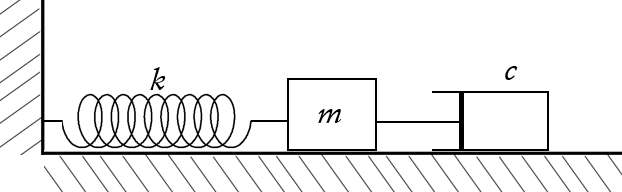
\includegraphics[scale=.9]{spring.PNG}}
\end{center}


We will assume that the floor is frictionless and the only friction force is caused by the dashpot. Using Newton's law $\sum F = ma$ we aim to derive an equation that governs the motion of the block.
In the picture, there are two kinds of forces: force of the spring and the friction force of the dashpot. Hence we have:
$$F_s + F_d = ma$$
For the spring, there is the Hooke's law, which states that
$$F_s = - kx$$
where $x$ is the displacement of the block from the equilibrium position. Notice that the $-$ sign is due to the fact that the spring always inserts force opposite of the displacement direction.
For the dashpot, the friction force tries to counter movement of the block. For example, if $v=0$ then there is no movement and therefore the dashpot doesn't exert any force. When $v$ is large, i.e. if the block tries move fast, the dashpot will exert a huge friction force in order to counter the velocity. This fact can be written as the following equation
$$F_d = -c v$$
where the negative sign means that the friction always tries to counter the direction of motion.
If we replace $F_s$ and $F_d$ with the equations we found, we get:
$$-kx -cv = ma$$
which is equivalent to:
$$ma +cv + kx =0$$
Now, consider the fact that velocity $v$ is the rate of change of displacement $x$, and that acceleration $a$ is the rate of change of velocity $v$. Thus above equation can be written as:
$$m x'' +c x' + kx=0$$
This is the differential equation for the motion of the block. When describing vibration of an object, often one can find an analogue of a spring-mass-dashpot system\index{spring-mass-dashpot system}. For example, the mechanical vibration of a car as it runs on the road has the mass as the mass of the car and the struts as springs (and various mechanical friction as dashpot). So the above equation has a quite universal application for describing \textbf{mechanical vibration\index{mechanical vibration}}.

\subsection*{In case of external force}
Suppose we have some external force $F_E$ applied to the block in addition to the spring force and the friction force. Then $\sum F = ma$ means:
$$F_E +F_s + F_d =ma$$
$$F_E - kx -cv =ma$$
$$F_E = mx'' + cx'+kx$$
This last equation is the differential equation to use when there is an external force acting on the block. Usually $F_E$ is not constant but a force that varies with time. So one writes $F_E (t)$ and we have:
$$F_E (t) = mx'' + cx'+kx$$

\subsection*{Over-damped, critically-damped and under-damped}

In case of no external force, the differential equation $m x'' -c x' + kx=0$ can be solved easily by using the characteristic equation:
$$mr^2 + cr +k =0$$
Using the quadratic formula,
$$r = \frac{-c \pm \sqrt{c^2 -4mk}}{2m}$$
Now, depending on the sign of what's inside the square root, there are 3 different cases that produce different kinds of solutions to $m x'' -c x' + kx=0$.

\begin{itemize}
	\item Case $c^2 -4mk>0$ \\
Then $r = \frac{-c \pm \sqrt{c^2 -4mk}}{2m}$ gives us two real solutions, $r= r_1$ and $r = r_2$. Which leads to :
$$x = C_1 e^{r_1 t}+C_2 e^{r_2 t}$$
We call this case \textbf{over-damped\index{over-damped}}

\item Case $c^2 -4mk=0$ \\
Then $r = \frac{-c \pm \sqrt{c^2 -4mk}}{2m}=\frac{-c}{2m}$ gives us a double root $r= r_1$. Which leads to :
$$x = C_1 e^{r_1 t}+C_2 t e^{r_1 t}$$
We call this case \textbf{critically damped\index{critically damped}}

\item Case $c^2 -4mk<0$ \\
Then $r = \frac{-c \pm \sqrt{c^2 -4mk}}{2m}$ gives us a complex root of the form $r= -a\pm wi$. Which leads to:
$$x = e^{-at} (C_1 \cos wt + C_2 \sin wt) $$
We call this case \textbf{under-damped\index{under-damped}}.

\end{itemize}

\subsection*{Undamped mechanical vibration}

The master equation for mechanical vibration is:
$$F(t) = mx'' + cx'+kx,$$
where $F(t)$ is the external force, $m$ is the mass, $c$ is the friction coefficient and $k$ is the spring constant.
Undamped motion is when there is no friction in the system, i.e. $c=0$. Let's investigate when there is no external force, so that we have:
$$m x'' + kx =0$$

To solve this, first write the characteristic equation
$$m r^2 +k =0 $$
$$r^2 = -\frac{k}{m}$$
$$r = \pm \sqrt{-\frac{k}{m}}$$
$$ r = \pm \sqrt{\frac{k}{m}}i$$
If we set
$$\omega = \sqrt{\frac{k}{m}},$$
then $r = \pm \omega i $, and the solution is:
$$x(t) = C_1 \cos \omega t + C_2 \sin \omega t$$
Note that both $\cos \omega t$ and $\sin \omega t$ are periodic functions with period
$$T = \frac{2\pi}{\omega}.$$
(One way to understand the above formula is to think about the special case when $\omega=1$. Then $\cos \omega t = \cos t$ which we know to have the period of $2\pi$.)
Now, since frequency $f=\frac{1}{T}$, we can further write:
$$T=\frac{1}{f}=\frac{2\pi}{\omega}.$$
Another useful formula you can obtain from above is
$$\omega = 2\pi f$$
This formula tells us what $\omega$ to choose when the frequency is given. $\omega$ is called the \textbf{angular frequency\index{angular frequency}}. Solving this for $f$ and also using $\omega = \sqrt{\frac{k}{m}}$, we have
$$f = \frac{1}{2\pi} \sqrt{\frac{k}{m}}$$
Above formula states that the frequency of the mechanical vibration depends on the mass and spring constant. More specifically, frequency is inversely proportional to the $\sqrt{m}$ while it is proportional to $\sqrt{k}$. This can be easily understood if you think about a heavy object (one with big value for $m$), for it will move slowly, causing the frequency to go down.

\subsection*{Putting $C_1 \cos \omega t + C_2 \sin \omega t$ into a single cosine function}

Graphs of $A\sin (at+b)$ and $A\cos (at+b)$ are called 'sinusoidal' because they have the same shape as the graph of $\sin t$. When two sinusoidal functions of \textit{same angular frequency} are added, the resulting function is again a sinusoidal function with the same angular frequency.

Say we have a sum of a sine and a cosine function of the same angular frequency, i.e.
$$A \cos \omega t + B\sin \omega t$$

Then we have the following formula:
$$A \cos \omega t + B\sin \omega t = C \cos (\omega t -\alpha),$$
where $C = \sqrt{A^2 + B^2} $ and $\alpha = \tan^{-1} \left(\frac{B}{A}\right) + \theta$ where $\theta$ depends on which quadrant the point $(A,B)$ belongs to, as shown in the picture below:

\begin{center}
	\makebox[\textwidth]{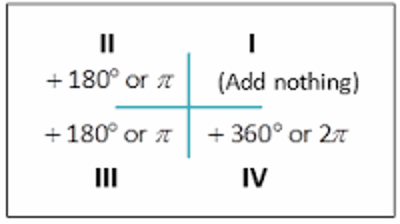
\includegraphics[scale=0.5]{quadrant.PNG}}
\end{center}


This way of writing makes it easy to see that the result of the sum of sinusoidal functions of the same period is again a sinusoidal function. It also tells you the \textbf{amplitude\index{amplitude}} $C$ of the sum and also the \textbf{phase angle\index{phase angle}} $\alpha$. So \textit{when writing your answer to mechanical vibrations, always make it into a single cosine function using the above formula}.

\begin{ex}
Suppose a block of 4 kg is attached to a spring with spring constant 1N/m. There is no external force or friction in the system. If the spring was compressed by 2m and was pushed with 1m/s initial velocity to the right, find period, amplitude and phase angle of the motion.
\end{ex}
Solution)
The equation for the motion is:
$$ 4 x''+ 1\cdot x =0$$
while the initial condition is $x(0)=-2$ and $x'(0)=1$.
$$4 r^2 + 1 = 0$$
$$r^2 = -\frac{1}{4}$$
$$r = \pm \frac{1}{2} i$$
$$x(t) = C_1 \cos{\frac{1}{2} t} + C_2 \sin{\frac{1}{2} t}$$
$$-2 = x(0) = C_1\cdot 1 + C_2 \cdot 0$$
$$C_1 = -2$$
$$x'(t) = -\frac{1}{2}C_1 \sin{\frac{1}{2} t} + \frac{1}{2}C_2 \cos{\frac{1}{2} t}$$
$$1= x'(0)=\frac{1}{2}C_2$$
$$C_2 = 2$$
$$C= \sqrt{(-2)^2 + 2^2} = \sqrt{8}=2\sqrt{2}$$
$$\alpha= \tan^{-1} \left(\frac{2}{-2}\right) + \pi = -\frac{\pi}{4}+\pi = \frac{3\pi}{4}$$
$$x = 2\sqrt{2} \cos{\left(\frac{1}{2} t -\frac{3\pi}{4}\right)}$$
Answer: Amplitude is $2\sqrt{2}$. Phase angle is $\frac{3\pi}{4}$. Period is:
$$T = \frac{2\pi}{1/2}=4\pi$$

\subsection*{An example of mechanical vibration with damping}
\begin{ex}
A body of mass m=1/2 kg is attached to the end of a spring that is stretched 2 meters by a force of 100N. The body is also attached to a dashpot that provides 1N of resistance for each m/s of velocity. If the initial position is $x(0)=1$ and it was set in motion with $v(0)=-5$, find the position functions, its frequency and pseudo-period of motion. Also find the time lag and the times of its first four passages through the equilibrium.
\end{ex}

Solution)
$$F(t) = mx'' + cx'+kx,$$
with $m=1/2$ and $c=1$. Also, by the Hooke's law $F=kx$, we can write $100 = k\cdot 2$ and we get $k=50$. There is no external force indicated, so we have:
$$\frac{1}{2} x'' + x' + 50x =0$$
with $x(0)=1, v(0)=x'(0)=-5$
$$\frac{1}{2} r^2 +r +50=0$$
$$r^2 + 2r+100=0$$
$$(r+1)^2+99=0$$
$$r= -1 \pm \sqrt{99}i$$
Hence
$$x(t) = e^{-t} (C_1 \cos \sqrt{99} t +C_2 \sin \sqrt{99} t)$$
$$1 = x(0) = C_1$$
$$x'(t)= -e^{-t} (C_1 \cos \sqrt{99} t +C_2 \sin \sqrt{99} t)$$
$$+e^{-t} (-\sqrt{99}C_1 \sin \sqrt{99} t +\sqrt{99}C_2 \cos \sqrt{99} t)$$
$$-5= x'(0) = -C_1 + C_2\sqrt{99}$$
Hence $C_2=\frac{-4}{\sqrt{99}}$
Thus:
$$x(t) = e^{-t} ( \cos \sqrt{99} t -\frac{4}{\sqrt{99}}C_2 \sin \sqrt{99} t)$$
Now we have to put the thing inside the parenthesis as a single cosine function:
$$C=\sqrt{1^2 + \left(\frac{-4}{\sqrt{99}}\right)^2}=\sqrt{\frac{115}{\sqrt{99}}}$$
$$\alpha= \tan^{-1} \left(\frac{-4}{\sqrt{99}}\right) = -0.3822$$
Hence,
$$x(t) = \sqrt{\frac{115}{\sqrt{99}}} e^{-t} \cos(\sqrt{99} t -(-0.3822))$$
Note that this is not a periodic function because $e^{-t} $ multiplied to above means that the amplitude is decreasing. However, we still call the $\omega=\sqrt{99}$ as the \textbf{pseudo-angular frequency\index{pseudo-angular frequency}} and use that to compute the \textbf{pseudoperiod\index{pseudoperiod}}:
$$T = \frac{2\pi}{\sqrt{99}}$$
Also, what the question calls the 'time lag' is what is usally called the \textbf{phase shift\index{phase shift}}:
$$\delta = \frac{\alpha}{\omega}$$
(in other words, phase angle divided by the angular frequency gives you the phase shift)
So the time lag calculated is =-0.038 (seconds).
Finally, in order to know when the block crosses the equilibrium, one uses the fact that cosine is zero at $\pi/2, 3\pi/2, 5\pi/2, \cdots$.
Therefore, the first four times block crosses the equilibrium can be calculated when $t$ satisfies:
$$\sqrt{99} t +0.3822 = \pi/2, 3\pi/2, 5\pi/2, 7\pi/2$$
Solving this, we get $t=0.119961, 0.435201, 0.750944$ and $1.066687$.

\subsection*{Mechanical vibration with a periodic external force}

\begin{ex} Suppose $m=1$, $c=4$, and $k=8$ in a spring-dashpot-mass system. If a periodic external force of $F(t)= 3 \cos (5t)$ is applied, find the general solution and also the steady periodic solution
	\end{ex}
Solution)
$$ 1\cdot x''+ 4x'+8x = 3\cos(5t)$$
$$r^2+4r+8=0$$
$$(r+2)^2+4=0$$
$$r=-2\pm 2i$$
$$x_c = e^{-2t} (C_1 \cos 2t + C_2 \sin 2t)$$

We use the method of undetermined coefficients to find $x_p$:
$$x_p = A\cos 5t + B\sin 5t$$
$$x_p'= 5B\cos 5t -5A\sin 5t$$
$$x_p'' = -25A\cos 5t + -25B\sin 5t$$
Hence $x_p''+ 4x_p'+8x_p = (-17A+20B)\cos 5t + (-17B-20A)\sin 5t$. For this to equal to $3\cos(5t)$, we need:
$$-17A+20B = 3$$
$$20A+17B=0$$
Solving this, we get: $A= \frac{-51}{689}$ and $B=\frac{60}{689}$. So the general solution is:
$$x = x_c + x_p = e^{-2t} (C_1 \cos 2t + C_2 \sin 2t) - \frac{51}{689}\cos 5t + \frac{60}{689}\sin 5t$$

Now, notice that the $x_c$ has the $e^{-2t}$ attached to it, which means it will rapidly become close to zero as $t$ increases. So after some time, the $x_c$ becomes irrelevant. Therefore, when there is a periodic external force, the solution $x_c$ is called the \textbf{transient solution\index{transient solution}} and is written as $x_{tr}$. On the other hand, $x_p$ doesn't have the exponential function attached and therefore, it does not decay (in other words, it's steady). So $x_p$ is called \textbf{steady periodic solution\index{steady periodic solution}} and is written as $x_{sp}$.
Thus the steady periodic solution is:
$$x_{sp}(t) = - \frac{51}{689}\cos 5t + \frac{60}{689}\sin 5t$$
(Note: Often you'll be asked to find the amplitude and phase angle of the steady periodic solution. In that case you have to convert the above into a single cosine function. )

\subsection*{Resonance for undamped mechanical vibration.}

Suppose we have an undamped mechanical motion with a periodic external force as follows: 
$$mx''+kx=F_0\cos\omega t.$$
Now there is the \textbf{natural angular frequency\index{natural angular frequency}} of the spring-mass system, given by 
$$\omega_0 = \sqrt{\frac{k}{m}}.$$
(Notice that heavier the block is, slower it will move, and thus lower frequency it will have.)
On the other hand, $F_0 \cos \omega t$ is the external force with angular frequency $\omega$.
When $\omega=\omega_0$, i.e. when the external force's angular frequency matches the natural frequency of the system, we say that there is \textbf{resonance\index{resonance}} in the system. Let's look at two examples comparing with and without resonance:

\textit{Case of no resonance: $x+4x= \sin t$ }

Since $m=1$ and $k=4$, the natural angular frequency is $\omega_0 = \sqrt{4/1} = 2$. Since the external force $\sin t = \sin 1\cdot t$ has angular frequency $1$, it's angular frequency is different from the natural angular frequency. So we know that this is a case of no resonance. 

Let us solve this using method of undetermined coefficients. Plugging in $x+p= A \sin t$ on the left side, we find that $x_p = \frac{1}{3} \sin t$ is a particular solution.
Since the characteristic equation $r^2+4=0$  has the solution $r=\pm 2i$, the complementary solution is $C_1 \cos 2t + C_2 \sin 2t$.
Thus the general solution is $x=x_c+x_p = C_1 \cos 2t + C_2 \sin 2t+\frac{1}{3} \sin t$. Important aspect of the solution is that all the functions above are bounded functions.

\textit{Case of resonance: $x''+4x = \sin 2t $}

This time, because there is duplication (when doing method of undetermined coefficients), $x_p = t( A\cos 2t + B\sin 2t)$ must be used. Plugging this into the left side gives:
$$x_p''+4x_p = 2 (-2A \sin 2t + 2B \cos 2t)$$
Hence $-4A=1$, $4B=0$. Thus $x_p=-\frac{1}{4} t \cos 2t$ and
$$x=x_c+x_p = C_1 \cos 2t + C_2 \sin 2t-\frac{1}{4} t \cos 2t$$
Important thing here is that $-\frac{1}{4} t \cos 2t$ is an unbounded function, as you can see in the graph below:

\begin{center}
	\makebox[\textwidth]{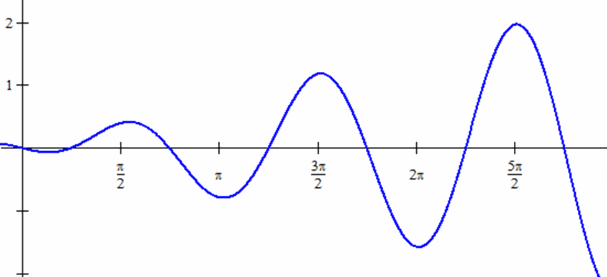
\includegraphics[width=0.7\textwidth]{resonance.PNG}}
\end{center}


In other words, if there is resonance, the resulting motion grows without bound. In the real world, this leads to bridges falling down, glasses breaking etc.

\subsection*{Practical Resonance for damped mechanical vibration }
Suppose we have a damped mechanical motion with a periodic external force as follows:
$$ mx'' + cx'+kx = F_0 \cos \omega t$$
Then we have learned that $x_c$ has a dying amplitude and thus is called the transient solution (written as $x_tr$) while $x_p= C \cos (\omega t - \alpha)$ is a periodic solution whose amplitude doesn't get smaller and thus is called the steady periodic solution (written as $x_sp$).
Using the method of undetermined coefficients, you can find that
$$x_sp = A\cos \omega t + B\sin \omega t,$$
with $A = \frac{(k-m\omega^2)F_0}{(k-m\omega^2)^2+(c\omega)^2}$ and $A = \frac{c\omega F_0}{(k-m\omega^2)^2+(c\omega)^2}$.

Using $C = \sqrt{A^2 + B^2} $ we get:
$$C= \frac{F_0}{\sqrt{(k-m\omega^2)^2+(c\omega)^2}}$$

If the value of $\omega$ is taken to make this amplitude to be maximized, we say that the external frequency has been tuned to practical resonance. It is the frequency when $x_sp$ has the largest amplitude, assuming $F_0$ is fixed.
To maximize $C$, we need the denominator to be minimized, which in turn is minimized when the radicand is minimized. Since minimum must occur at the critical point, we differentiate with respect to $\omega$:
$$\left((k-m\omega^2)^2+(c\omega)^2\right)'=0$$
$$2(k-m\omega^2)(-2m\omega)+ 2c^2 \omega =0$$

Find the angular frequency of the external force which creates practical resonance for the system with m=1, c=4 and k=10
solution)
$$C= \frac{F_0}{\sqrt{(k-m\omega^2)^2+(c\omega)^2}}= \frac{F_0}{\sqrt{(10-\omega^2)^2+(4\omega)^2}}$$
Then
$$\left((10-\omega^2)^2+(4\omega)^2\right)'=0$$
$$2(10-\omega^2)(-2\omega)+ 32 \omega =4\omega(\omega-2)=0$$
Thus the critical numbers are $\omega=0,2$ but we throw out $\omega=0$ because it is not physically possible.
Answer: $\omega=2$

\subsection*{Introduction to LCR circuits}

An LCR circuit (also called RLC, LRC, CRL ... ) is a circuit made of an inductor(with inductance L), a capacitor(with capacitance C) and a resistor (with resistance R) connected in a series to a voltage source $\mathcal{E} (t)$ as shown below:
\begin{center}
	\makebox[\textwidth]{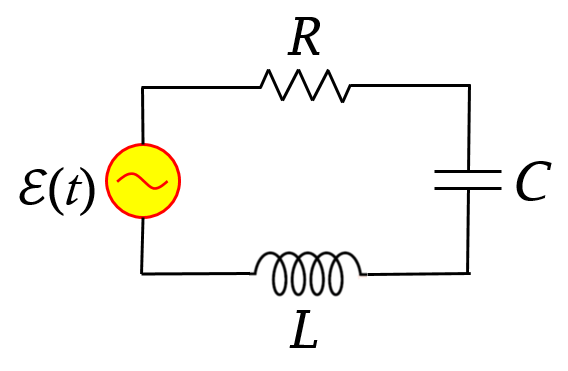
\includegraphics[width=0.3\textwidth]{LCR.PNG}}
\end{center}

Now the voltage drop across an inductor is $V_L = -L \frac{dI}{dt}$ because inductors try to counter the changes in current. Voltage drop across a resistor is $V_R= -IR$ which is called the Ohm's law. Lastly, the voltage drop across a capacitor is $V_C = - \frac{1}{C} Q$ where $Q$ is the charge. If the circuit is provided with the voltage of $\mathcal{E} (t)$, then using the Kirchoff's loop law (which states that the sum of voltages around a loop is zero), we have the following:
$$ \mathcal{E} (t)-L \frac{dI}{dt} -IR- \frac{1}{C} Q =0$$
or
$$ \mathcal{E} (t)=L \frac{dI}{dt} +IR + \frac{1}{C} Q $$
In the above, there are two unknown functions of time $t$. One is the current $I(t)$ and the other is the charge $Q(t)$. There is a relation between the two, because the current is the rate of the change of the charge, i.e. $I(t)= Q'(t)$.
So if we differentiate the differential equation, we get:
$$ \mathcal{E}' (t)=L I'' +R I' + \frac{1}{C} I $$
This equation is the master equation for LCR circuits.

Notice that this is a second order linear differential equation. You can compare this with the mechanical vibrations equation and find an analogy between $x(t)$ and $I(t)$. In fact, what $L$ is doing is exactly what $m$ is doing in mechanical vibration. $R$ corresponds to $c$ and $\frac{1}{C}$ corresponds to $k$. The $ \mathcal{E}' (t)$ acts like the external force. Therefore, everything you learned about the mechanical vibration applies to the LCR circuits. We can talk about under-damped, over-damped, and critically damped. We can talk about frequency, period and pseudo period. We can talk about transient solutions and steady periodic solutions, etc. In LCR circuits, the phase angle is an important quantity because it tells you how much the current is lagging or leading the input voltage.
Note about the lagging/leading: If the current peaks a little before the voltage, then we say the current 'leads' the voltage. The graph of the current then would be shifted left, which means the phase angle is negative. There could be a little confusion here because many books just write $C \cos(\omega t + \phi)$ so that what we are calling as $-\alpha$ is instead called $\phi$. In other words, if $\phi$ is positive, so that $\alpha$ is negative, then the current 'leads' the voltage.

\begin{ex}
Suppose R= 30 $\Omega$, L= 10 H, C = 0.02 F and $ \mathcal{E} (t) = 50 \sin 2t$ V. Find amplitude of the current and also how much the current is lagging or leading the voltage.
\end{ex}
Solution)
The equation is:
$$ 10 I + 30 I' + \frac{1}{0.02}I= 100 \cos 2t$$
Using the method of undetermined coefficients, setting $I_p= A \cos 2t + B \sin 2t$ and plugging it into the differential equation gives us that
$$y_p =\frac{10}{37}\cos 2t + \frac{60}{37}\sin 2t$$
Now,
$$C = \sqrt{ \left(\frac{10}{37}\right)^2+\left(\frac{60}{37}\right)^2 } = 1.644$$
and
$$\alpha = \tan^{-1} \frac{60/37}{10/37} = 1.406 \textrm{ rad}$$
So the current is lagging the voltage by 1.406 radians. The peak current is 1.644 amperes.

\chapter{Series Solutions to Differential Equations}
\section{Power Series Solutions}
\subsection*{Introduction to Series Solutions}

Consider the differential equation:
$$y'' - 3xy'+2y=0$$
This differential equation is quite different than what we have done so far, because there is a coefficient $-3x$ in front of $y'$ which makes it non-constant.
In the constant coefficient case, we made a 'guess' that the answer is in some format of $e^{rx}$. However, when the coefficient is not constant but rather a function of $x$, the solution quickly becomes very complicated and usually ends up being a function which cannot be expressed using polynomials, trigs, exponentials, logs or any other functions that we are used to.
Thus we need to use a completely different approach to this differential equation. The way we are going to solve it is by representing the solution as a power series\index{power series}.

\subsection*{Brief digression to power series}
Recall that $e^x$ can be represented by a power series:
$$e^x = 1 + x + \frac{1}{2!} x^2 + \frac{1}{3!} x^3 +\cdots$$
This is what we know as the Taylor series (or Maclaurin series) of $e^x$. Many functions that we know that is infinitely differentiable can be represented as a power series.
If your knowledge of power series is not quite there, you can get some understanding of the power series by considering two things.

First, the equal sign holds for all values of $x$ as long as the right side converges. This means, for $x=1$, we have:
$$e=e^1=1 + 1 + \frac{1}{2!} 1^2 + \frac{1}{3!} 1^3 + \frac{1}{4!} 1^4+\cdots$$
$$ \approx  1 + 1 + \frac{1}{2!} 1^2 + \frac{1}{3!} 1^3 + \frac{1}{4!} 1^4 \approx 2.70833$$
In other words, if we took the first 5 terms of the series we get the above approximation. Considering that $e=2.7182818...$, the above is a pretty good approximation. In fact, if you take more terms, more accurate the approximation will be.

Second, you have to know how this power series is obtained. Suppose all that you know is that $e^x$ can be written as a power series. Then you may write:
$$e^x = a_0 + a_1 x + a_2 x^2 +a_3 x^3 +\cdots$$
However, we don't know what the coefficients $a_0, a_1, a_2, \cdots $ are. So we have to figure out what they are. The idea is to understand that the above equation is an equation for functions, which means (a) it should hold for any value of $x$ and (b) even if you differentiate both sides the two sides are still equal. To get $a_0$, we plug in $x=0$ to get:
$$e^0 = a_0 + a_1 \cdot 0 + a_2 \cdot 0^2 +a_3 \cdot 0^3 +\cdots $$
$$1 = a_0$$
Then we differentiate both sides:
$$e^x = a_1  + 2 a_2 x + 3a_3 x^2 + 4a_4 x^3 +\cdots$$
Again, plug in $x=0$ to get:
$$e^0 = a_1  + 2 a_2 \cdot 0 + 3a_3 \cdot 0^2 + 4a_4 \cdot 0^3 +\cdots$$
$$1 = a_1$$
Differentiate more:
$$e^x = 2 a_2  + 3\cdot 2 a_3 x + 4\cdot 3a_4 x^2 + 5\cdot 4a_5 x^3+\cdots$$
Again, plug in $x=0$ to get:
$$e^0 = 2 a_2  + 3\cdot 2 a_3 \cdot 0 + 4\cdot 3a_4 \cdot 0^2 + 5\cdot 4a_5 \cdot 0^3+\cdots$$
$$1 = 2 a_2$$
$$a_2 = \frac{1}{2}$$
We can continue this until there is a pattern. Taylor series (or Maclaurin series) is basically this packaged as an easy-to-use formula.

\subsection*{Back to the differential equation}
Once again we owe to the mathematicians who proved the existence of the solutions of differential equations such as:
$$y'' - 3xy'+2y=0$$
Because we know that the general solution exists, we can think about its Taylor series. In other words, we take $y$ to be:
$$y = \sum_{n=0}^{\infty} a_n x^{n} $$
The above is equivalent to saying $y=a_0 + a_1 x + a_2 x^2 +a_3 x^3 +\cdots$. It's written in sigma notation.
To plug it into the differential equation, we have to differentiate:
$$y' = \sum_{n=1}^{\infty} n a_n x^{n-1} $$
Notice that the summation starts with $n=1$. This is because if $y=a_0 + a_1 x + a_2 x^2 +a_3 x^3 +\cdots$ is differentiated, you get $y=a_0 + a_1 x + a_2 x^2 +a_3 x^3 +\cdots$ which means the $a_0$ term disappears. So $n$ has to start from 1. Likewise:
$$y'' = \sum_{n=2}^{\infty} n (n-1) a_n x^{n-2} $$
starts from $n=2$.
We plug this into the differential equation to get the following:
$$y'' - 3xy'+2y= \sum_{n=2}^{\infty} n (n-1) a_n x^{n-2} -3x \sum_{n=1}^{\infty} n a_n x^{n-1}+2\sum_{n=0}^{\infty} a_n x^{n}$$
Things multiplied in front of $\sum$ can be brought into the $\sum$. So that:
$$= \sum_{n=2}^{\infty} n (n-1) a_n x^{n-2} + \sum_{n=1}^{\infty} (-3x)n a_n x^{n-1}+\sum_{n=0}^{\infty} 2a_n x^{n}$$
$$= \sum_{n=2}^{\infty} n (n-1) a_n x^{n-2} + \sum_{n=1}^{\infty} -3 n a_n x^{n}+\sum_{n=0}^{\infty} 2a_n x^{n}$$

\subsection*{Shifting}
Notice that in the term $\sum_{n=2}^{\infty} n (n-1) a_n x^{n-2}$, the exponent of $x^{n-2}$ is $n-2$, while for the other to $\sum$'s they are $n$. For the reason that will be clear later, you want to match the exponents over $x$, and that technique is called \textit{shifting\index{shifting of indices}} of indices. Here is what it is: Take the $\sum_{n=2}^{\infty} n (n-1) a_n x^{n-2}$. Since we want the exponent to be $n$, we replace the $n$ in $x^{n-2}$ by $n+2$, so that $x^{n-2}$ becomes $x^{n+2-2}=x^{n}$. But when you do that, you have to change every $n$ in the summation $\sum_{n=2}^{\infty} n (n-1) a_n x^{n-2}$, even including the $n=2$ in the bottom.


$n=2$ is transformed like this: Since we are replacing $n$ by $n+2$, it becomes $n+2=2$. But then if you solve for $n$, you have $n=0$.
After replacing $n$ by $n+2$, the summation $\sum_{n=2}^{\infty} n (n-1) a_n x^{n-2}$ becomes $\sum_{n=0}^{\infty} (n+2) (n+1) a_{n+2} x^{n}$. Now this \textit{shifting} is complete. After the shifting, this is what we have:
$$y'' - 3xy'+2y=\sum_{n=0}^{\infty} (n+2) (n+1) a_{n+2} x^{n} + \sum_{n=1}^{\infty} -3 n a_n x^{n}+\sum_{n=0}^{\infty} 2a_n x^{n}$$

\subsection*{Introduction to Series Solutions}

In the previous section, we went over the technique of shifting. You should check that the summation after the shifting produces the exact same terms as what you had before the shifting. So we are not changing anything, but just the way it's written.
Let's look at what we have again:
$$y'' - 3xy'+2y= \sum_{n=0}^{\infty} (n+2) (n+1) a_{n+2} x^{n} + \sum_{n=1}^{\infty} -3 n a_n x^{n}+\sum_{n=0}^{\infty} 2a_n x^{n}$$
There are three summations you see here. Summations are things that produce terms, e.g. $\sum_{n=0}^{\infty} (n+2) (n+1) a_{n+2} x^{n}$ produces $2\cdot 1 \cdot a_2 x^0$ when $n=0$. Then it produces $3\cdot 2 \cdot a_3 x^1$ when $n=1$.
So basically you have three term-producing factories working. There is a difference in when they start their work though. When $n=0$, only the first and the last factories (i.e. summations) produce terms. But then, starting from $n=1$ and afterwards, all factories are working to produce terms.
Let's make use of this observation by separating out the terms produced when $n=0$ as follows:
$$=2\cdot 1 \cdot a_2 x^0+2a_0x^0 + \sum_{n=1}^{\infty} (n+2) (n+1) a_{n+2} x^{n} + \sum_{n=1}^{\infty} -3 n a_n x^{n}+\sum_{n=1}^{\infty} 2a_n x^{n}$$
Then the three sums can be put together as a single sum as:
$$=2\cdot 1 \cdot a_2 x^0+2a_0x^0 + \sum_{n=1}^{\infty} \left( (n+2) (n+1) a_{n+2} x^{n} +  -3 n a_n x^{n}+ 2a_n x^{n} \right)$$
Then factor out $x^n$ to get:
$$=(2\cdot 1 \cdot a_2+2a_0) x^0 + \sum_{n=1}^{\infty} \left( (n+2) (n+1) a_{n+2}  +  -3 n a_n + 2a_n  \right)x^{n}$$
Now, this has to equal to zero, because $y'' - 3xy'+2y=0$ that we are trying to solve has zero on the right. When you have a power series organized in terms of power of $x$ which has to equal to zero, it is a mathematical theorem that each coefficient has to equal to zero (the reason being that the Taylor series of zero is $0+0\cdot x+0\cdot x^2\cdots$.) and hence we have the following identities:
$$ 2\cdot 1 \cdot a_2+2a_0=0$$
$$ (n+2) (n+1) a_{n+2}  +  (2-3 n) a_n =0 $$
The first equation gives us $a_2 = -a_0$. The second equation holds for $n=1$ and afterwards. When you solve the second one by $a_{n+2}$ you have
$$ a_{n+2} = \frac{3n-2}{(n+2) (n+1)} a_n, \; \; n\geq 1 $$
This is called the \textit{recurrence relation} because it could be used over and over again.
Let's think about the consequences of the recurrence relation. When $n=1$,
$$a_3 = \frac{1}{6} a_1 $$
Then when $n=2$,
$$a_4 = \frac{4}{12} a_2$$
But since $a_2 = -a_0$ we have:
$$a_4 = - \frac{1}{3} a_0$$
Then when $n=3$,
$$a_5 = \frac{7}{20} a_3 = \frac{7}{120} a_1 $$
You can see that all the $a_n$ can be represented by using either $a_0$ or $a_1$ (or sometimes both). This is good because we know that at the end of the day there should be two free parameters. $a_0$ and $a_1$ will end up being the free parameters.

Already we have some idea of the power series solution\index{power series solution} for $y$:
$$y= a_0 + a_1 x + a_2 x^2 +a_3 x^3 +a_4 x^4+a_5 x^5 +\cdots$$
$$=a_0 + a_1 x - a_0 x^2 + \frac{1}{6} a_1 x^3 - \frac{1}{3} a_0 x^4+\frac{7}{120} a_1 x^5 +\cdots$$
The above is a significant result because $a_0$ and $a_1$ can be determined if the initial condition is given. When they are determined, the above will tell us the few terms of the power series expansion (a.k.a. Taylor series) of $y$, which can be used to find approximate value of $y$ when $x$ is near $0$.

\subsection*{Example of a series solution to a differential equation. }

\begin{ex}
$$(x^2+3)y'' +4xy'+y =0$$
\end{ex}
Solution)
It is important to \textit{expand before solving by series}:
$$x^2 y'' + 3y'' + 4xy'+y=0$$
Then write $y$ as power series:
$$y = \sum_{n=0}^{\infty} a_n x^{n} $$
$$y' = \sum_{n=1}^{\infty} n a_n x^{n-1} $$
$$y'' = \sum_{n=2}^{\infty} n (n-1) a_n x^{n-2} $$
(When doing power series solutions, the above is always used.)
Plugging into the left side of $(x^2+3)y'' +4xy'+y =0$ we get:
$$x^2 \sum_{n=2}^{\infty} n (n-1) a_n x^{n-2}+ 3 \sum_{n=2}^{\infty} n (n-1) a_n x^{n-2} + 4x\sum_{n=1}^{\infty} n a_n x^{n-1} + \sum_{n=0}^{\infty} a_n x^{n}$$
$$ = \sum_{n=2}^{\infty} n (n-1) a_n x^{n}+ \sum_{n=2}^{\infty} 3n (n-1) a_n x^{n-2} + \sum_{n=1}^{\infty} 4n a_n x^{n} + \sum_{n=0}^{\infty} a_n x^{n}$$
In the four summations above, everything has $x^n$ except for the second, so we shift the second summation by replacing $n$ by $n+2$:
$$\sum_{n=2}^{\infty} 3n (n-1) a_n x^{n-2} = \sum_{n=0}^{\infty} 3(n+2) (n+1) a_{n+2} x^{n}$$
Hence we have:
$$\sum_{n=2}^{\infty} n (n-1) a_n x^{n}+ \sum_{n=0}^{\infty} 3(n+2) (n+1) a_{n+2} x^{n} + \sum_{n=1}^{\infty} 4n a_n x^{n} + \sum_{n=0}^{\infty} a_n x^{n}$$
We look at each summation and see that the second and fourth summations begin at $n=0$, and that starting from $n=2$ and afterwards all summations produce terms. So we write:
$$ =(6a_2+a_0)x^0 + (18a_3+ 4a_1 + a_1)x^1 + \sum_{n=0}^{\infty} \left( n (n-1) a_n +3(n+2) (n+1) a_{n+2} + 4n a_n +a_n \right)x^n $$
Since the above has to equal to zero on the right side of $(x^2+3)y'' +4xy'+y =0$, we obtain the following equations:
$$6a_2+a_0=0$$
$$ 18a_3+ 4a_1 + a_1=0$$
$$ n (n-1) a_n +3(n+2) (n+1) a_{n+2} + 4n a_n +a_n =0 $$
The first two equations yield $a_2 = -\frac{1}{6} a_0 $ and $a_3 = -\frac{5}{18}a_1$. The third equation, which holds for $n \geq 2$, solved for $a_{n+2}$ gives us:
$$a_{n+2} = - \frac{n^2+ 3n +1}{3(n+2) (n+1)} a_n, \; \; \; n\geq 2$$
This last equation is called the \textit{recurrence relation}. We use the recurrence relation to get the following results:
$$n=2 \; \rightarrow \; a_4=- \frac{11}{36} a_2=  \frac{11}{216} a_0$$
$$n=3 \; \rightarrow \; a_5=- \frac{19}{60} a_3=  \frac{19}{216} a_1$$
and so on.
So the answer, the first six non-zero terms of $y$ is:
$$y= a_0 + a_1 x -\frac{1}{6} a_0 x^2 -\frac{5}{18}a_1 x^3 + \frac{11}{216} a_0x^4+\frac{19}{216} a_1 x^5 +\cdots$$

\subsection*{Power series solution when initial condition is given }

\begin{ex}
$$y'' + xy'+ y =0, \; \; y(0)=1, y'(0)=-2 $$
\end{ex}
Solution)
Let's think about what the initial conditions mean. Since $y=a_0 + a_1 x + a_2 x^2 +a_3 x^3 +\cdots$, the initial condition $y(0)=1$ means $1=y(0)= a_0 + a_1 \cdot 0  + a_2 \cdot 0^2 +a_3 \cdot 0^3 +\cdots = a_0$. In other words, $y(0)$ \textit{gives you the value of} $a_0$.
Also, $y' = a_1  + 2 a_2 x + 3a_3 x^2 + 4a_4 x^3 +\cdots$ and $y'(0)=-2$ means
$-2 = y'(0) = a_1  + 2 a_2 \cdot 0 + 3a_3 \cdot 0^2 + 4a_4 \cdot 0^3 +\cdots = a_1$.
Therefore, we find that $a_0=1$ and $a_1=-2$.
Note: If the value of $y''(0)$ is given, then $a_2$ will be equal to half of that. (Why?)

Other than this part, the rest is solved exactly like before.
$$y = \sum_{n=0}^{\infty} a_n x^{n} $$
$$y' = \sum_{n=1}^{\infty} n a_n x^{n-1} $$
$$y'' = \sum_{n=2}^{\infty} n (n-1) a_n x^{n-2} $$
Plugging these into the left side of $y'' + xy'+ y =0$ yields:
$$ \sum_{n=2}^{\infty} n (n-1) a_n x^{n-2} + x \sum_{n=1}^{\infty} n a_n x^{n-1}  + \sum_{n=0}^{\infty} a_n x^{n} $$
$$ = \sum_{n=2}^{\infty} n (n-1) a_n x^{n-2} +  \sum_{n=1}^{\infty} n a_n x^{n}  + \sum_{n=0}^{\infty} a_n x^{n} $$
$$ = \sum_{n=0}^{\infty} (n+2)(n+1) a_{n+2} x^{n} +  \sum_{n=1}^{\infty} n a_n x^{n}  + \sum_{n=0}^{\infty} a_n x^{n} $$
$$ = (2a_2+a_0)x^0 + \sum_{n=1}^{\infty} \left( (n+2)(n+1) a_{n+2}+n a_n+a_n \right) x^n $$
Therefore,
$$2a_2+a_0=0 \; \rightarrow \; a_2 = -\frac{1}{2}a_0 = -\frac{1}{2} $$
$$ (n+2)(n+1) a_{n+2}+n a_n+a_n =0$$
$$ \rightarrow \; a_{n+2} = -\frac{1}{n+2} a_n, \; (n\geq 1) $$
Using the recurrence relation above:
$$n=1 \; \rightarrow \; a_3 = -\frac{1}{3} a_1 = \frac{2}{3}$$
$$n=2 \; \rightarrow \; a_4 = -\frac{1}{4} a_2 = -\frac{1}{8}$$
$$n=3 \; \rightarrow \; a_5 = -\frac{1}{5} a_3 = -\frac{2}{15}$$
Hence the first 6 non-zero terms of the solution are:
$$y = 1 -2x -\frac{1}{2} x^2+ \frac{2}{3} x^3 - \frac{1}{8} x^4 -  -\frac{2}{15} x^5 \cdots $$

\section{Frobenius Method }

\subsection*{Limitations of the power series}
Although power series can express most of the functions we know, it does miss some of the desired functions, such as $\frac{1}{x(1-x)}$. This function cannot have a power series expansion because the derivative does not exist at $x=0$.
However, you can have something similar to a power series:
Since $\frac{a}{1-r} = a + ar + ar^2 + ar^3 + \cdots$, taking $a=1$ and $r=x$, we have:
$$\frac{1}{1-x} = 1 + x + x^2 + x^3 + \cdots $$
Then we have:
$$\frac{1}{x(1-x)}= \frac{1}{x}\cdot \frac{1}{(1-x)} = \frac{1}{x} ( 1 + x + x^2 + x^3 + \cdots) = x^{-1} ( 1 + x + x^2 + x^3 + \cdots)  $$

Mathematician Ferdinand Frobenius realized that if one puts $x^r$ multiplied to a power series, it can express many more kinds of functions. His method is called the \textbf{Frobenius Method\index{Frobenius Method}}, which is to use the following form as the form of the solution:
$$y= x^r (a_0 + a_1x + a_2 x^2 + a_3 x^3 + \cdots ) = x^r \sum_{n=0}^{\infty} a_n x^n $$
Here, if $r=0$, it's the usual power series. By a \textbf{Frobenius solution}, we are talking about solutions where $r$ is negative or a fraction and $a_0 \neq 0$. Those solutions cannot be expressed using just a power series. When do a differential equation have power series solutions and when do a differential equation have a Frobenius solution? The answer to this requires the understanding of singular and ordinary points of a differential equation, and we will discuss it later. Before that, let's look at an example where Frobenius solution is required:

\begin{ex}
$$2x^2 y'' + 3xy' - (x^2 +1)y =0$$
\end{ex}
Solution)
Use the Frobenius form of the solution:
$$y = x^r \sum_{n=0}^{\infty} a_n x^n  = \sum_{n=0}^{\infty} a_n x^{n+r}$$
$$y' = \sum_{n=0}^{\infty} (n+r)a_n x^{n+r-1}$$
$$y'' = \sum_{n=0}^{\infty} (n+r)(n+r-1)a_n x^{n+r-2}$$
\textbf{Important}: In the $y'$, no longer you start the summation from $n=1$. That's because in a Frobenius solution, the series does not start from the constant term, and therefore the first term does not become zero when differentiated. Same goes for $y''$.

Now, let's plug in to the left side:
$$2x^2 y'' + 3xy' - x^2y- y =2x^2 \sum_{n=0}^{\infty} (n+r)(n+r-1)a_n x^{n+r-2} + 3x\sum_{n=0}^{\infty} (n+r)a_n x^{n+r-1} - x^2\sum_{n=0}^{\infty} a_n x^{n+r} -\sum_{n=0}^{\infty} a_n x^{n+r}$$
$$= \sum_{n=0}^{\infty} 2(n+r)(n+r-1)a_n x^{n+r} + \sum_{n=0}^{\infty} 3(n+r)a_n x^{n+r} - \sum_{n=0}^{\infty} a_n x^{n+r+2} -\sum_{n=0}^{\infty} a_n x^{n+r}$$
Let us shift the third summation by replacing $n$ by $n-2$.
$$= \sum_{n=0}^{\infty} 2(n+r)(n+r-1)a_n x^{n+r} + \sum_{n=0}^{\infty} 3(n+r)a_n x^{n+r} - \sum_{n=2}^{\infty} a_{n-2} x^{n+r} -\sum_{n=0}^{\infty} a_n x^{n+r}$$
$$= (2(r-1)ra_0 + 3ra_0 - a_0)x^r +  (2r(r+1)a_1 + 3(r+1)a_1 - a_1)x^{r+1} $$
$$ \qquad \qquad \qquad \qquad +  \sum_{n=2}^{\infty} \left( 2(n+r)(n+r-1)a_n +  3(n+r)a_n - a_{n-2} - a_n \right) x^{n+r} $$
So we have
$$ 2(r-1)ra_0 + 3ra_0 - a_0=0 $$
$$ 2r(r+1)a_1 + 3(r+1)a_1 - a_1 = 0 $$
$$ 2(n+r)(n+r-1)a_n +  3(n+r)a_n - a_{n-2} - a_n =0 \;  ,  \qquad (n\geq 2)$$

Until now, you may think that this is not much different than power series solutions. Indeed so far there is not much difference. However, the very first equation you get has an interesting property:
$$ 2(r^2-r)a_0 + 3ra_0 - a_0=0 \; \rightarrow \; (2r^2+r-1)a_0 =0 $$
This means either $(2r^2+r-1)=0$ or $a_0 =0 $. Here is when we use the important condition that the very first term of the solution shouldn't be zero (the condition we wrote above that $a_0 \neq 0$. ) Because $a_0 \neq 0$, the only choice we have is $(2r^2+r-1)=0$. The value of $r$ is called the \textit{index} of the solution and the equation we got for $r$ is called the \textit{indicial equation}. Later, we will find out how to get the indicial equation quickly. Anyways, here is the indicial equation:
$$2r^2 + r -1=0$$
$$(2r-1)(r+1)=0$$
$$r = \frac{1}{2}, -1 $$
\textit{Each value of $r$ will lead to different (i.e. linearly independent) Frobenius solution} provided that they do not differ by an integer. If they do differ by an integer, the higher value of $r$ always provides a Frobenius solution, while the lower value may or may not give us a Frobenius solution. Since solving linear second order differential equation requires finding two linearly independent solutions, if the second solution is not of the Frobenius form, it has to be found in some other way. Luckily, it turns out that in such a case, the second solution can be found in the following form:
$$y_2 = C y_1 \ln x + \sum_{n=0}^{\infty} b_n x^{k+r_2} , $$
where $y_1$ is the Frobenius solution corresponding to the larger root $r_1$, and $r_2$ is the smaller root. Such a solution is called an extended Frobenius solution \index{Frobenius solution, extended}. 

\subsection*{Introduction to Frobenius Method part 2 }
Let's choose $r = \frac{1}{2} $ and carry on with the calculation. The other two equations we had were:
$$ 2r(r+1)a_1 + 3(r+1)a_1 - a_1 = 0 $$
$$ 2(n+r)(n+r-1)a_n +  3(n+r)a_n - a_{n-2} - a_n =0 \;  ,  \; n\geq 2$$
which simplifies to:
$$ (2r^2+ 5r +2 )a_1 = 0 $$
$$ \left( 2(n+r)(n+r-1) + 3(n+r) -1 \right)a_n  = a_{n-2}  \;  ,  \; n\geq 2$$
With the chosen value $r = \frac{1}{2} $, we get:

$$2 a_1 =0 $$
$$ \left( 2(n+\frac{1}{2})(n-\frac{1}{2}) + 3n +\frac{3}{2}-1 \right) a_n  = a_{n-2}  \;  ,  \; n\geq 2$$
So we have $a_1=0$ and
$$ \left( 2n^2 +3n \right) a_n  = a_{n-2}  \;  ,  \; n\geq 2$$
$$ a_n = \frac{1}{n(2n + 3)} a_{n-2}  \;  ,  \; n\geq 2$$
This is the recurrence relation.

Let's try to find the first four non-zero terms using the recurrence relation:
$$a_2 = \frac{1}{2\cdot 7} a_{0} = \frac{1}{14} a_{0} $$
$$a_3 = \frac{1}{3\cdot 9} a_{1} = 0 $$
(since $a_1=0$. In fact, all the odd items will be zero.)
$$a_4 = \frac{1}{4\cdot 11} a_{2} = \frac{1}{616} a_{0} $$
$$a_6 = \frac{1}{6\cdot 15} a_{4} = \frac{1}{55440} a_{0} $$

Hence:
$$y = x^{1/2} \left( a_0 + \frac{1}{14} a_{0} x^2 + \frac{1}{616} a_{0} x^4 + \frac{1}{55440} a_{0} x^6 \dots \right)= a_0 x^{1/2}  \left( 1+ \frac{1}{14}  x^2 + \frac{1}{616} x^4 + \frac{1}{55440} x^6 \dots \right)$$
is the solution obtained. Now, since $a_0$ is arbitrary we can choose $a_0=1$ and find that one solution obtained for $r=\frac{1}{2}$ is:
$$y_1 = x^{1/2}  \left( 1+ \frac{1}{14}  x^2 + \frac{1}{616} x^4 + \frac{1}{55440} x^6 \dots \right)$$
But since we are solving second order linear differential equation, we need two linearly independent solutions. So we have to find the second solution by putting $r=-1$. We go back to 
$$ 2r(r+1)a_1 + 3(r+1)a_1 - a_1 = 0 $$
$$ 2(n+r)(n+r-1)a_n +  3(n+r)a_n - a_{n-2} - a_n =0 \;  ,  \; n\geq 2$$
We plug in $r=-1$ and get
$$ - a_1 = 0 $$
$$ 2(n-1)(n-2)a_n +  3(n-1)a_n - a_{n-2} - a_n =0 \;  ,  \; n\geq 2$$
(Note that these $a_n$'s are not the same ones we obtained for the case $r=\frac{1}{2}$.) Thus we have $a_1=0$ and 
$$ \left( 2(n^2-3n+2)+3n-3 -1 \right) a_n = a_{n-2}\;  ,  \; n\geq 2$$
$$ a_n = \frac{1}{2n^2 -3n} a_{n-2}\;  ,  \; n\geq 2$$
This is the recurrence relation. 

Let's try to find the first four non-zero terms using the recurrence relation:
$$a_2 = \frac{1}{2} a_{0}  $$
$$a_3 = \frac{1}{9} a_{1} = 0 $$
(since $a_1=0$. In fact, all the odd items will be zero.)
$$a_4 = \frac{1}{20} a_{2} = \frac{1}{40} a_{0} $$
$$a_6 = \frac{1}{54} a_{4} = \frac{1}{2160} a_{0} $$

Hence:
$$y = x^{-1} \left( a_0 + \frac{1}{2} a_{0} x^2 + \frac{1}{40} a_{0} x^4 + \frac{1}{2160} a_{0} x^6 \dots \right) = a_0 x^{-1} \left( 1 + \frac{1}{2} x^2 + \frac{1}{40} x^4 + \frac{1}{2160} x^6 \dots \right)$$

Again, set $a_0=1$ to get the second solution:
$$y_2 = x^{-1} \left( 1 + \frac{1}{2} x^2 + \frac{1}{40} x^4 + \frac{1}{2160} x^6 \dots \right) $$

Now take the linear combination of the two solutions $y_1$ and $y_2$ to get the full solution:

$$y = C_1 x^{1/2}  \left( 1+ \frac{1}{14}  x^2 + \frac{1}{616} x^4 + \frac{1}{55440} x^6 \dots \right) + C_2 x^{-1} \left( 1 + \frac{1}{2} x^2 + \frac{1}{40} x^4 + \frac{1}{2160} x^6 \dots \right) $$

Note: The fact that $y_1$ and $y_2$ are linearly independent can be most easily proved by looking at the asymptotic behavior of the function near zero, but the proof will be omitted since asymptotic behavior lies beyond the scope of this book. 

\subsection*{Why power series solutions not good for singular differential equation }
We will learn that the equation $2x^2 y'' + 3xy' - (x^2 +1)y =0$ has $x=0$ as a singular point. But before we learn about that, we will try to see what goes wrong if one tried to find a power series solution to this equation.

Let us try to look for the power series form of $y$ as a solution to $2x^2 y'' + 3xy' - (x^2 +1)y =0$. This means:
$$y = \sum_{n=0}^{\infty} a_n x^{n} $$
$$y' = \sum_{n=1}^{\infty} n a_n x^{n-1} $$
$$y'' = \sum_{n=2}^{\infty} n (n-1) a_n x^{n-2} $$
Plugging this in, we get:
$$2x^2 y'' + 3xy' - x^2y- y =2x^2 \sum_{n=2}^{\infty} n (n-1) a_n x^{n-2} + 3x\sum_{n=1}^{\infty} n a_n x^{n-1} - x^2\sum_{n=0}^{\infty} a_n x^{n} -\sum_{n=0}^{\infty} a_n x^{n}$$
$$= \sum_{n=2}^{\infty} 2 n (n-1) a_n x^{n} + \sum_{n=1}^{\infty} 3n a_n x^{n} - \sum_{n=0}^{\infty} a_n x^{n+2} -\sum_{n=0}^{\infty} a_n x^{n}$$
$$= \sum_{n=2}^{\infty} 2 n (n-1) a_n x^{n} + \sum_{n=1}^{\infty} 3n a_n x^{n} - \sum_{n=2}^{\infty} a_{n-2} x^{n} -\sum_{n=0}^{\infty} a_n x^{n}$$
$$ = a_0 x^0 + (3a_1 +a_1) x^1 + \sum_{n=2}^{\infty} \left( 2 n (n-1) a_n + 3n a_n - a_{n-2} -a_n \right) x^n $$
Then we have:
$$a_0 =0 $$
$$3a_1 +a_1=0 \; \rightarrow \; a_1 =0 $$
$$ 2 n (n-1) a_n + 3n a_n - a_{n-2} -a_n = 0 \; \rightarrow \; \left( 2n^2 +n -1 \right)a_n = a_{n-2} \; , \; n \geq 2 $$
So the recurrence relation is:
$$a_n = \frac{1}{2n^2 +n -1} a_{n-2}\;, \; n \geq 2$$
Let's plug in values of $n$:
$$n=2 \; \rightarrow \; a_2 = \frac{1}{9} a_{0} =0 $$
$$n=3 \; \rightarrow \; a_3 = \frac{1}{20} a_{1} =0 $$
$$n=4 \; \rightarrow \; a_4 = \frac{1}{35} a_{2} =0 $$
As you can see, all $a_n$ will turn out to be zero, yielding the solution $y=0$. Such answer is called the \textit{trivial solution} because any homogeneous differential equation will have zero as one answer (which is a useless answer in most cases.)


\subsection*{Regular singular points and irregular singular points }
Here is how to get the index $r$ quickly. Let's use the same example as before:
$$2x^2 y'' + 3xy' - (x^2 +1)y =0$$
Dividing by $2x^2$ gives us:
$$ y'' + \frac{3x}{2x^2} y' - \frac{x^2 +1 }{2x^2} y = 0 $$
Now, any second order homogeneous differential equation can be turned into the following form:
$$ y'' + P(x) y' + Q(x) y =0 $$
if you divide by what's in front of $y''$ (which in the above case we had $2x^2$).
Comparing, we see that $P(x) = \frac{3x}{2x^2} = \frac{3}{2x} $ and $ Q(x) = - \frac{x^2 +1 }{2x^2} $. \textit{You must include the sign when you figure out } $P(x)$ and $Q(x)$.

There are some important concepts you have to know before we go for the indicial equations:
\begin{itemize}
\item When, after simplifying $P(x)$ and $Q(x)$, both $P(0)$ and $Q(0)$ are well defined , we say $x=0$ is a \textbf{ordinary point\index{ordinary point}} of the differential equation.
\item When, after simplifying $P(x)$ and $Q(x)$, if any or both of $P(0)$ and $Q(0)$ are undefined (i.e. $x=0$ causes the denominator to become zero) then we say $x=0$ is a \textbf{singular point\index{singular point}} of the differential equation.
\end{itemize}

Now, if the differential equation is singular at $x=0$, we define $p(x)$ and $q(x)$ as :
$$p(x) = x P(x) \; , \; q(x) = x^2 Q(x) $$

If $p(0)$ and $q(0)$ are well defined, we say the differential equation has a \textbf{regular singular point\index{regular singular point}} at $x=0$. If not, $x=0$ is said to be an \textbf{irregular singular point\index{irregular singular point}}. In other words, singular points come in two flavors - regular and irregular.

Here is what's known: If $x=0$ is ordinary, then the differential equation can be solved by power series. If $x=0$ is regular singular, then the differential equation can be solved by Frobenius method. If it is irregular singular, then Frobenius nor the power series method will work.

\subsection*{Indicial equation}
Once $p(x)$ and $q(x)$ are calculated, the \textbf{indicial equation \index{indicial equation}} is:
$$r (r-1) + p(0)r + q(0) =0$$

In the above example,
$$p(x) = x P(x) = x \cdot \frac{3}{2x} = \frac{3}{2} $$
$$q(x) = x^2 Q(x) = x^2 \cdot \frac{x^2 +1 }{2x^2}  = \frac{x^2 +1 }{2} $$
Hence $p(0) =  \frac{3}{2} $ and $q(0) = \frac{1}{2} $, and we have:
$$r(r-1) + \frac{3}{2} r + \frac{1}{2} = 0 $$
Multiplying by $2$ and simplifying gives us $2r^2 + r -1=0$, exactly same as what we had before.


\begin{ex}
	$$2x^2 y'' + (7x-x^2) y' + 2y =0 $$
\end{ex}

Solution) First divide by $2x^2$ to make it into the standard form:
$$ y'' + \frac{7x-x^2}{2x^2} y' + \frac{1}{x^2} y =0 $$
We see that $P(x)=\frac{x(7-x)}{2x^2}$ and $Q(x)= \frac{1}{x^2}$. Hence
$$p(x) = x P(x) = \frac{7-x}{2} \; \; ,  q(x) = x^2 Q(x) = 1 \; \; \rightarrow p_0=p(0)=\frac{7}{2} \;, q_0=q(0)= 1$$
This makes the indicial equation
$$r(r-1) + \frac{7}{2} r + 1 = 0 \; \; \rightarrow \; \; r^2 + \frac{5}{2}r + 1 =0 $$
Multiplying the equation by $2$, we have $2r^2 + 5r + 2 =0$. Using the quadratic formula, we have
$$ r= \frac{-5 \pm \sqrt{25-4\cdot 2\cdot 2}}{2\cdot 2} = \frac{-5 \pm 3}{4} \rightarrow r= -2 \; , \; -\frac{1}{2}  $$ 
	
Since the two numbers $-2$ and $-\frac{1}{2}$ do not differ by a constant, both of them yield a Frobenius solution. Let us find the Frobenius solution for each case.

But before we do so, we will rewrite the differential equation $2x^2 y'' + (7x-x^2) y' + 2y =0 $ as 
$$2x^2 y'' + 7x y' -x^2y' + 2y =0 $$
You will see that this format is easier. 

\textbf{Case } $r=-2$

$$y = x^r \sum_{n=0}^{\infty} a_n x^n  = \sum_{n=0}^{\infty} a_n x^{n+(-2)}$$
We differentiate twice:
$$y' = \sum_{n=0}^{\infty} (n-2) a_n x^{n-3} $$
$$y'' = \sum_{n=0}^{\infty} (n-2)(n-3) a_n x^{n-4} $$
(Note that contrary to the case when deriving power series solutions, during Frobenius method we don't change $n=0$ to $n=1$ or $n=2$ when taking derivatives.)

Now plug in these formulas into $2x^2 y'' + 7x y' -x^2y' + 2y =0 $:
$$ 2x^2  \sum_{n=0}^{\infty} (n-2)(n-3) a_n x^{n-4} + 7x  \sum_{n=0}^{\infty} (n-2) a_n x^{n-3} - x^2  \sum_{n=0}^{\infty} (n-2) a_n x^{n-3} + 2 \sum_{n=0}^{\infty} a_n x^{n-2} = 0$$
$$ \sum_{n=0}^{\infty} 2(n-2)(n-3) a_n x^{n-2} +   \sum_{n=0}^{\infty} 7(n-2) a_n x^{n-2} -  \sum_{n=0}^{\infty} (n-2) a_n x^{n-1} + 2 \sum_{n=0}^{\infty} a_n x^{n-2} = 0$$

We see that the second from the last summation needs shifting of indices. For that summation only, we replace $n$ by $n-1$ so that:
$$\sum_{n=0}^{\infty} (n-2) a_n x^{n-1} \; \; \rightarrow \; \sum_{n=1}^{\infty} (n-3) a_{n-1} x^{n-2}  $$
Note that the $n=1$ in the bottom is due to changing $n=0$ to $n-1=0$ which is equivalent to $n=1$. The resulting summation is 
$$ \sum_{n=0}^{\infty} 2(n-2)(n-3) a_n x^{n-2} +   \sum_{n=0}^{\infty} 7(n-2) a_n x^{n-2} -  \sum_{n=1}^{\infty} (n-3) a_{n-1} x^{n-2}  + 2 \sum_{n=0}^{\infty} a_n x^{n-2} = 0$$

Now, when $n=0$, the shifted summation does not produce any terms because that one begins with $n=1$, while the other summations produce terms. We can separate out the terms produced when $n=0$ and rewrite it as:
$$ 2(-2)(-3)a_0 x^{-2} +  7(-2)a_0 x^{-2} + 2 a_0 x^{-2}\qquad \qquad \qquad \qquad \qquad \qquad \qquad \qquad \qquad \qquad$$
$$ \qquad \qquad \qquad + \sum_{n=1}^{\infty} 2(n-2)(n-3) a_n x^{n-2} +   \sum_{n=1}^{\infty} 7(n-2) a_n x^{n-2} -  \sum_{n=1}^{\infty} (n-3) a_{n-1} x^{n-2}  + 2 \sum_{n=1}^{\infty} a_n x^{n-2} = 0$$
But $  2(-2)(-3)a_0 x^{-2} +  7(-2)a_0 x^{-2} + 2 a_0 x^{-2} = (12a_0 -14a_0 + 2a_0)x^{-2} =0$. Hence it cancels away. Also, since all the summations now begin at $n=1$, we can just use a single summation to express all the sums at once:

$$\sum_{n=1}^{\infty} \left( 2(n-2)(n-3) a_n x^{n-2} +    7(n-2) a_n x^{n-2} -   (n-3) a_{n-1} x^{n-2}  + 2 a_n x^{n-2} \right)= 0$$

$$\sum_{n=1}^{\infty} \left( 2(n-2)(n-3) a_n  +    7(n-2) a_n -   (n-3) a_{n-1}   + 2 a_n  \right) x^{n-2} = 0$$

Thus we must have:
$$ 2(n-2)(n-3) a_n  +    7(n-2) a_n -   (n-3) a_{n-1}   + 2 a_n  = 0$$
$$ \left( 2(n-2)(n-3)  + 7(n-2)  + 2 \right) a_n = (n-3) a_{n-1}$$
$$ \left( 2n^2 -10n +12 +7n -14 +2 \right) a_n = (n-3) a_{n-1}$$
$$ \left( 2n^2 - 3n \right) a_n = (n-3) a_{n-1}$$
$$ a_n = \frac{n-3}{n(2n-3)} a_{n-1} \; \; , \; (n\geq 1)$$

This leads to:
$$ a_1 = {-2}{1\cdot (-1)} a_0=2a_0 $$
$$ a_2 = \frac{-1}{2\cdot 1} a_1 = -\frac{1}{2} a_1 = -\frac{1}{2}\cdot 2 a_0 = -a_0 $$
$$a_3 = \frac{0}{3\cdot 3} a_2 =0$$
But then $a_4 = (something) a_3 =0$ and $a_5$ is zero for the same reason, and we end up with all $a_n=0$ after $n\geq 3$.

Hence the solution is:

$$y = x^{-2} \left( a_0 + a_1 x + a_2 x^2 + a_3 x^3 +\cdots \right) = x^{-2} \left( a_0 + 2a_0 x -a_0 x^2 + 0 +0+ \cdots \right)$$
$$y = a_0 x^{-2} \left(1+2x-x^2\right) = a_0 \left( \frac{1}{x^2} + \frac{2}{x} -1 \right) $$

\textbf{Case } $r=-\frac{1}{2}$

$$y = x^r \sum_{n=0}^{\infty} a_n x^n  = \sum_{n=0}^{\infty} a_n x^{n+(-1/2)}$$
We differentiate twice:
$$y' = \sum_{n=0}^{\infty} \left(n-\frac{1}{2} \right) a_n x^{n-3/2} $$
$$y'' = \sum_{n=0}^{\infty} \left(n-\frac{1}{2} \right)\left(n-\frac{3}{2} \right) a_n x^{n-5/2} $$

Now plug in these formulas into $2x^2 y'' + 7x y' -x^2y' + 2y =0 $:
$$ 2x^2  \sum_{n=0}^{\infty} \left(n-\frac{1}{2} \right)\left(n-\frac{3}{2} \right) a_n x^{n-5/2} + 7x  \sum_{n=0}^{\infty} \left(n-\frac{1}{2} \right) a_n x^{n-3/2} - x^2  \sum_{n=0}^{\infty} \left(n-\frac{1}{2} \right) a_n x^{n-3/2} + 2 \sum_{n=0}^{\infty} a_n x^{n-1/2} = 0$$
$$ \sum_{n=0}^{\infty} 2\left(n-\frac{1}{2} \right)\left(n-\frac{3}{2} \right) a_n x^{n-1/2} +  \sum_{n=0}^{\infty} 7\left(n-\frac{1}{2} \right) a_n x^{n-1/2} -   \sum_{n=0}^{\infty} \left(n-\frac{1}{2} \right) a_n x^{n+1/2} + \sum_{n=0}^{\infty} 2a_n x^{n-1/2} = 0$$

We see that the second from the last summation needs shifting of indices. For that summation only, we replace $n$ by $n-1$ so that:
$$\sum_{n=0}^{\infty} \left(n-\frac{1}{2} \right) a_n x^{n+1/2} \; \; \rightarrow \; \sum_{n=1}^{\infty} \left(n-\frac{3}{2} \right) a_{n-1} x^{n-1/2} $$
Note that the $n=1$ in the bottom is due to changing $n=0$ to $n-1=0$ which is equivalent to $n=1$. The resulting summation is 
$$ \sum_{n=0}^{\infty} 2\left(n-\frac{1}{2} \right)\left(n-\frac{3}{2} \right) a_n x^{n-1/2} +  \sum_{n=0}^{\infty} 7\left(n-\frac{1}{2} \right) a_n x^{n-1/2} -   \sum_{n=1}^{\infty} \left(n-\frac{3}{2} \right) a_{n-1} x^{n-1/2} + \sum_{n=0}^{\infty} 2a_n x^{n-1/2} = 0$$

Now, when $n=0$, the shifted summation does not produce any terms because that one begins with $n=1$, while the other summations produce terms. We can separate out the terms produced when $n=0$ and rewrite it as:
$$ 2(-\frac{1}{2})(-\frac{3}{2})a_0 x^{-1/2} +  7(-\frac{1}{2})a_0 x^{-1/2} + 2 a_0 x^{-1/2}\qquad \qquad \qquad \qquad \qquad \qquad \qquad \qquad \qquad \qquad$$
$$ \qquad \qquad \qquad + \sum_{n=1}^{\infty} 2\left(n-\frac{1}{2} \right)\left(n-\frac{3}{2} \right) a_n x^{n-1/2} +  \sum_{n=1}^{\infty} 7\left(n-\frac{1}{2} \right) a_n x^{n-1/2} -   \sum_{n=1}^{\infty} \left(n-\frac{3}{2} \right) a_{n-1} x^{n-1/2} + \sum_{n=1}^{\infty} 2a_n x^{n-1/2} = 0$$
But $  2(-\frac{1}{2})(-\frac{3}{2})a_0 x^{-1/2} +  7(-\frac{1}{2})a_0 x^{-1/2} + 2 a_0 x^{-1/2} = (\frac{3}{2} a_0 -\frac{7}{2}a_0 + 2a_0)x^{-1/2} =0$. Hence it cancels away. Also, since all the summations now begin at $n=1$, we can just use a single summation to express all the sums at once:

$$\sum_{n=1}^{\infty} 2\left(n-\frac{1}{2} \right)\left(n-\frac{3}{2} \right) a_n x^{n-1/2} +   7\left(n-\frac{1}{2} \right) a_n x^{n-1/2} -  \left(n-\frac{3}{2} \right) a_{n-1} x^{n-1/2} + 2a_n x^{n-1/2} = 0$$

$$\sum_{n=1}^{\infty} \left( 2\left(n-\frac{1}{2} \right)\left(n-\frac{3}{2} \right) a_n +   7\left(n-\frac{1}{2} \right) a_n -  \left(n-\frac{3}{2} \right) a_{n-1}  + 2a_n \right) x^{n-1/2} = 0$$

Thus we must have:
$$ 2\left(n-\frac{1}{2} \right)\left(n-\frac{3}{2} \right) a_n +   7\left(n-\frac{1}{2} \right) a_n -  \left(n-\frac{3}{2} \right) a_{n-1}  + 2a_n   = 0$$
Multiplying $2$ both sides gets rid of denominators as:
$$ (2n-1)(2n-3)a_n +   (14n-7) a_n -  (2n-3) a_{n-1}  + 4a_n   = 0$$
$$ (2n-1)(2n-3)a_n +   (14n-7) a_n  + 4a_n   =  (2n-3) a_{n-1}$$
$$ \left( 4n^2 -8n + 3 +14n -7 + 4 \right) a_n = (2n-3) a_{n-1}$$
$$ \left( 4n^2 +6n  \right) a_n = (2n-3) a_{n-1}$$
$$ a_n = \frac{2n-3}{2n(2n+3)} a_{n-1} \; \; , \; (n\geq 1)$$

This leads to:
$$ a_1 = {-1}{2\cdot 5} a_0= -\frac{1}{10} a_0 $$
$$ a_2 = \frac{1}{4\cdot 7} a_1 = \frac{1}{28} a_1 = \frac{1}{28} \cdot \left(-\frac{1}{10} a_0 \right) = - \frac{1}{280} a_0 $$
$$a_3 = \frac{3}{6\cdot 9} a_2 =  \frac{1}{18} a_2 = \frac{1}{18}\cdot \left(-\frac{1}{280} a_0 \right) = - \frac{1}{5040} a_0 $$

$$a_4 =  \frac{5}{8\cdot 11 } a_2 = - \frac{1}{88704} a_0 $$


Hence the solution is:

$$y = x^{-1/2} \left( a_0 + a_1 x + a_2 x^2 + a_3 x^3 +\cdots \right) = x^{-1/2} \left( a_0  -\frac{1}{10} a_0 x - \frac{1}{280} a_0 x^2  - \frac{1}{5040} a_0 x^3  - \frac{1}{88704} a_0 x^4 + \cdots \right)$$
$$y = a_0 x^{-1/2} \left(1  -\frac{1}{10} x - \frac{1}{280} x^2  - \frac{1}{5040} x^3  - \frac{1}{88704} x^4 + \cdots  \right) $$

Now taking the linear combinations of the two solutions obtained for $r=-2$ and $r=-\frac{1}{2}$, we get:
$$y= C_1 \left( \frac{1}{x^2} + \frac{2}{x} -1 \right) + C_2 x^{-1/2} \left(1  -\frac{1}{10} x - \frac{1}{280} x^2  - \frac{1}{5040} x^3  - \frac{1}{88704} x^4 + \cdots  \right) $$

\subsection*{Case when the two roots of the indicial equation differ by an integer}

\begin{ex}
$$x^2 y'' + 5xy' + (3-x) y =0$$
\end{ex}

First divide by $x^2$ to make it into the standard form:

$$ y'' + \frac{5}{x} y' + \frac{3-x}{x^2} y =0 $$
We see that $P(x)=\frac{5}{x}$ and $Q(x)= \frac{3-x}{x^2}$. Hence
$$p(x) = x P(x) = 5 \; \; ,  q(x) = x^2 Q(x) = 3-x \; \; \rightarrow p_0=p(0)=5 \;, q_0=q(0)= 3$$
This makes the indicial equation
$$r(r-1) + 5 r + 3 = 0 \; \; \rightarrow \; \; r^2 + 4r + 3 =0 $$
The equation $ r^2 + 4r + 3 =0$ can be factored as $(r+3)(r+1)=0$, and hence $r=-3$ or $r=-1$

\textbf{Case } $r=-1$

$$y = x^r \sum_{n=0}^{\infty} a_n x^n  = \sum_{n=0}^{\infty} a_n x^{n+(-1)}$$
We differentiate twice:
$$y' = \sum_{n=0}^{\infty} (n-1) a_n x^{n-2} $$
$$y'' = \sum_{n=0}^{\infty} (n-1)(n-2) a_n x^{n-3} $$
(Note that contrary to the case when deriving power series solutions, during Frobenius method we don't change $n=0$ to $n=1$ or $n=2$ when taking derivatives.)

Now rewrite the given equation $x^2 y'' + 5xy' + (3-x) y =0$ as $x^2 y'' + 5xy' + 3y -xy =0$ and plug in these formulas:
$$ x^2  \sum_{n=0}^{\infty} (n-1)(n-2) a_n x^{n-3} + 5x \sum_{n=0}^{\infty} (n-1) a_n x^{n-2} + 3 \sum_{n=0}^{\infty} a_n x^{n-1} - x  \sum_{n=0}^{\infty} a_n x^{n-1} = 0$$
$$  \sum_{n=0}^{\infty} (n-1)(n-2) a_n x^{n-1} + 5 \sum_{n=0}^{\infty} (n-1) a_n x^{n-1} + 3 \sum_{n=0}^{\infty} a_n x^{n-1} - \sum_{n=0}^{\infty} a_n x^{n} = 0$$

We see that the last summation needs shifting of indices. For that last summation only, we replace $n$ by $n-1$ so that:
$$\sum_{n=0}^{\infty} a_n x^{n} \; \; \rightarrow \; \sum_{n=1}^{\infty} a_{n-1} x^{n-1}  $$
Note that the $n=1$ in the bottom is due to changing $n=0$ to $n-1=0$ which is equivalent to $n=1$. The resulting summation is 
$$  \sum_{n=0}^{\infty} (n-1)(n-2) a_n x^{n-1} + 5 \sum_{n=0}^{\infty} (n-1) a_n x^{n-1} + 3 \sum_{n=0}^{\infty} a_n x^{n-1} - \sum_{n=1}^{\infty} a_{n-1} x^{n-1} = 0 $$

Now, when $n=0$, only the first three summations produce terms and the last summation is at rest. (The last one only begins producing terms when $n=1$.) We can separate out the terms produced when $n=0$ and rewrite it as:
$$ (-1)(-2)a_0 x^{-1} + 5\cdot (-1)a_0 x^{-1} + 3a_0 x^{-1}\qquad \qquad \qquad \qquad \qquad \qquad \qquad \qquad \qquad \qquad$$
$$ \qquad \qquad \qquad + \sum_{n=1}^{\infty} (n-1)(n-2) a_n x^{n-1} + 5 \sum_{n=1}^{\infty} (n-1) a_n x^{n-1} + 3 \sum_{n=1}^{\infty} a_n x^{n-1} - \sum_{n=1}^{\infty} a_{n-1} x^{n-1} = 0 $$
But $ (-1)(-2)a_0x^{-1} + 5\cdot (-1)a_0 x^{-1}+ 3a_0 x^{-1} = (2a_0 -5a_0 + 3a_0)x^{-1} =0$. Hence it cancels away. Also, since all the summations now begin at $n=1$, we can just use a single summation to express all the sums at once:

$$\sum_{n=1}^{\infty} \left( (n-1)(n-2) a_n x^{n-1} + 5 (n-1) a_n x^{n-1} + 3 a_n x^{n-1} - a_{n-1} x^{n-1} \right)= 0$$

$$\sum_{n=1}^{\infty} \left((n-1)(n-2) a_n + 5 (n-1) a_n + 3 a_n  -a_{n-1} \right) x^{n-1} = 0$$

Thus we must have:
$$ (n-1)(n-2) a_n + 5 (n-1) a_n + 3 a_n  -a_{n-1} = 0$$
$$ \left( (n-1)(n-2) + 5 (n-1) + 3 \right) a_n = a_{n-1}$$
$$ a_n = \frac{1}{(n-1)(n-2) + 5 (n-1) + 3} a_{n-1} $$
$$ a_n = \frac{1}{n(n+2)} a_{n-1} \; \; , \; (n\geq 1)$$

This leads to:
$$ a_1 = \frac{1}{2\cdot 3} a_0 $$
$$ a_2 = \frac{1}{3\cdot 4} a_1 = \frac{1}{3\cdot 4}\cdot \frac{1}{2\cdot 3} a_0 = \frac{1}{(3\cdot2) (4\cdot 3 )} a_0 $$
$$a_3 = \frac{1}{4\cdot 5} a_2 = \frac{1}{4\cdot 5}\cdot \frac{1}{(3\cdot2) (4\cdot 3 )} a_0 = \frac{1}{(4\cdot 3\cdot2) (5 \cdot 4\cdot 3 )} a_0 $$
We see that a pattern emerges. We can write $(4\cdot 3\cdot2)=4!$ and $(5 \cdot 4\cdot 3 )= \frac{5!}{2}$ so that:
$$a_3 = \frac{2}{4!5!} a_0 $$
In general, the pattern is:
$$a_n = \frac{2}{(n+1)!(n+2)!} a_0 \; \; , \; (n\geq 1)$$
Notice that the above is true even when $n=0$, because $\frac{2}{(0+1)!(0+2)!} a_0 = \frac{2}{2}a_0 = a_0$. So we can take the above as a solution for all $a_n$. Thus the solution is:

$$y = \sum_{n=0}^{\infty} \frac{2}{(n+1)!(n+2)!} a_0 x^{n-1} = a_0 \sum_{n=0}^{\infty} \frac{2}{(n+1)!(n+2)!} x^{n-1}$$

\textbf{Case } $r=-3$

$$y = x^r \sum_{n=0}^{\infty} a_n x^n  = \sum_{n=0}^{\infty} a_n x^{n+(-3)}$$
We differentiate twice:
$$y' = \sum_{n=0}^{\infty} (n-3) a_n x^{n-4} $$
$$y'' = \sum_{n=0}^{\infty} (n-3)(n-4) a_n x^{n-5} $$


Now rewrite the given equation $x^2 y'' + 5xy' + (3-x) y =0$ as $x^2 y'' + 5xy' + 3y -xy =0$ and plug in these formulas:
$$ x^2  \sum_{n=0}^{\infty} (n-3)(n-4) a_n x^{n-5} + 5x \sum_{n=0}^{\infty} (n-3) a_n x^{n-4} + 3 \sum_{n=0}^{\infty} a_n x^{n-3} - x  \sum_{n=0}^{\infty} a_n x^{n-3} = 0$$

$$  \sum_{n=0}^{\infty} (n-3)(n-4) a_n x^{n-3} + 5 \sum_{n=0}^{\infty} (n-3) a_n x^{n-3} + 3 \sum_{n=0}^{\infty} a_n x^{n-3} - \sum_{n=0}^{\infty} a_n x^{n-2} = 0$$

We see that the last summation needs shifting of indices. For that last summation only, we replace $n$ by $n-1$ so that:
$$\sum_{n=0}^{\infty} a_n x^{n-2} \; \; \rightarrow \; \sum_{n=1}^{\infty} a_{n-1} x^{n-3}  $$
Note that the $n=1$ in the bottom is due to changing $n=0$ to $n-1=0$ which is equivalent to $n=1$. The resulting summation is 

$$  \sum_{n=0}^{\infty} (n-3)(n-4) a_n x^{n-3} + 5 \sum_{n=0}^{\infty} (n-3) a_n x^{n-3} + 3 \sum_{n=0}^{\infty} a_n x^{n-3} - \sum_{n=1}^{\infty} a_{n-1} x^{n-3} = 0$$

Now, when $n=0$, only the first three summations produce terms and the last summation is at rest. (The last one only begins producing terms when $n=1$.) We can separate out the terms produced when $n=0$ and rewrite it as:
$$ (-3)(-4)a_0 x^{-3} + 5\cdot (-3)a_0 x^{-3} + 3a_0 x^{-3}\qquad \qquad \qquad \qquad \qquad \qquad \qquad \qquad \qquad \qquad$$
$$ \qquad \qquad \qquad + \sum_{n=1}^{\infty} (n-3)(n-4) a_n x^{n-3} + 5 \sum_{n=1}^{\infty} (n-3) a_n x^{n-3} + 3 \sum_{n=1}^{\infty} a_n x^{n-3} - \sum_{n=1}^{\infty} a_{n-1} x^{n-3} = 0 $$
But $ (-3)(-4)a_0 x^{-3} + 5\cdot (-3)a_0 x^{-3} + 3a_0 x^{-3} = (12a_0 -15a_0 + 3a_0)x^{-3} =0$. Hence it cancels away. Also, since all the summations now begin at $n=1$, we can just use a single summation to express all the sums at once:

$$\sum_{n=1}^{\infty} \left( (n-3)(n-4) a_n x^{n-3} + 5 (n-3) a_n x^{n-3} + 3 a_n x^{n-3} - a_{n-1} x^{n-3} \right)= 0$$

$$\sum_{n=1}^{\infty} \left( (n-3)(n-4) a_n + 5 (n-3) a_n + 3 a_n - a_{n-1} \right)  x^{n-3}= 0$$

Thus we must have:
$$ (n-3)(n-4) a_n + 5 (n-3) a_n + 3 a_n  -a_{n-1} = 0$$
$$ \left( (n-3)(n-4) + 5 (n-3) + 3 \right) a_n = a_{n-1}$$
$$ a_n = \frac{1}{(n-3)(n-4) + 5 (n-3) + 3} a_{n-1} $$
$$ a_n = \frac{1}{n(n-2)} a_{n-1} \; \; , \; (n\geq 1)$$

\textbf{Until now, this solution may look exactly like the solution we wrote for } $r=-1$. However, notice that $ a_n = \frac{1}{n(n-2)} a_{n-1}$ is not defined for $n=2$, because we get a $0$ in the denominator. That is why there is no Frobenius solution corresponding to $r=-3$. 


\chapter{System of Differential Equations}
\section{Introduction to System of Differential Equations}

\subsection*{Introduction to system of differential equations (part I)}

Suppose we have a system of differential equations:
$$\begin{cases} x+2y=x' \\ 4x+3y =y' \end{cases}$$
with initial condition $x(0)=1 \; , \; y(0)=3$. In the above, $x$ and $y$ are functions of $t$ and the derivatives are with respect to $t$. This means we are looking for two functions $x(t)$ and $y(t)$ that satisfy the above differential equations and initial conditions.

We can put the system into a matrix notation as follows:
$$\begin{pmatrix} x \\ y \\ \end{pmatrix}' = \begin{pmatrix} 1 & 2 \\ 4 & 3 \\ \end{pmatrix}  \begin{pmatrix} x \\ y \\ \end{pmatrix} $$

After the system is changed into the matrix form, it can be solved using a related problem in matrices called the eigenvector problem.

\subsection*{Eigenvalues and eigenvectors}
A matrix that is made up of a single column, e.g.
$$\begin{pmatrix} a \\ b \\ \end{pmatrix} $$
is called a column vector.

For a given matrix $\mathbf{A}$, an \textbf{eigenvector\index{eigenvector}} of $\mathbf{A}$ is a non-zero column vector $\mathbf{v}$ satisfying $\mathbf{A}\mathbf{v} = \lambda \mathbf{v}$ for some constant $\lambda$. For example, if we consider the eigenvector of the matrix appearing in the above system of differential equations, it means we are looking to find numbers $a, \; b$ and $\lambda$ that satisfy:
$$\begin{pmatrix} 1&2 \\ 4& 3\\ \end{pmatrix} \begin{pmatrix} a \\ b\\ \end{pmatrix} = \lambda \begin{pmatrix} a \\ b\\ \end{pmatrix} $$
In the above, vector $\mathbf{v}$ is the column vector made of $a$ and $b$, and the condition that $\mathbf{v}$ should be non-zero means that \textit{at least one of $a$ and $b$ should be non-zero.} The value of $\lambda$ that satisfies the above equation is called the \textbf{eigenvalue\index{eigenvalue}} associated to the eigenvector $\mathbf{v}$.

Let's try to find what $a, \; b$ and $\lambda$ can satisfy the above matrix equation. First, multiply the left side:
$$\begin{pmatrix} a+2b \\ 4a+ 3b\\ \end{pmatrix} =  \begin{pmatrix} \lambda a \\ \lambda b\\ \end{pmatrix} $$
Now, the above is equivalent to the following system:
$$\begin{cases} a+2b=\lambda a  \\ 4a+ 3b= \lambda b \end{cases}$$
We can treat this equation as an equation of $a$ and $b$. Move $\lambda a$ to the left and group it with $a$. Also move $\lambda b$ to the left and group it with $3b$. We end up with:
$$\begin{cases} (1-\lambda)a+2b =0  \\ 4a+ (3-\lambda)b= 0 \end{cases}$$
Now let's go back to matrix form as:
$$\begin{pmatrix} 1- \lambda &2 \\ 4& 3- \lambda\\ \end{pmatrix} \begin{pmatrix} a \\ b\\ \end{pmatrix} =  \begin{pmatrix} 0 \\ 0\\ \end{pmatrix} $$

This has an easy solution. Just multiply the inverse matrices to both sides:
$$\begin{pmatrix} 1- \lambda &2 \\ 4& 3- \lambda\\ \end{pmatrix}^{-1} \begin{pmatrix} 1- \lambda &2 \\ 4& 3- \lambda\\ \end{pmatrix} \begin{pmatrix} a \\ b\\ \end{pmatrix} =  \begin{pmatrix} 1- \lambda &2 \\ 4& 3- \lambda\\ \end{pmatrix}^{-1} \begin{pmatrix} 0 \\ 0\\ \end{pmatrix} $$
Then there is a cancellation on the left side, while on the right, anything times zero matrix is zero:
$$\begin{pmatrix} a \\ b\\ \end{pmatrix} =  \begin{pmatrix} 0 \\ 0\\ \end{pmatrix} $$

BUT WAIT! We are not supposed to have both $a$ and $b$ equal to zero!

So what went wrong? The only way this solution could go wrong is when the inverse matrix does not exist. (Since we want at least one of $a$ and $b$ to be non-zero, we want it to go wrong - then there is a chance that we could have at least one of $a$ and $b$ to be non-zero. )

So when does a matrix NOT have an inverse? That's when the determinant is zero, i.e.
$$\begin{vmatrix} 1- \lambda &2 \\ 4& 3- \lambda\\ \end{vmatrix}=0$$
Computing the determinant, we have:
$$(1- \lambda)(3- \lambda) - 2 \cdot 4 =0$$
$$ \lambda^2 - 4 \lambda -5 =0$$
$$ (\lambda -5)(\lambda +1) =0$$

So far our conclusion means this: The only way we could have a non-zero $a$ and $b$ is when $\lambda = 5$ or $\lambda =-1$

Now what we need is to figure out what $a$ and $b$ could be for each value of $\lambda$.

\begin{itemize}
\item  Case $\lambda = 5 $
\end{itemize}
We plug the value into:
$$\begin{pmatrix} 1- \lambda &2 \\ 4& 3- \lambda\\ \end{pmatrix} \begin{pmatrix} a \\ b\\ \end{pmatrix} =  \begin{pmatrix} 0 \\ 0\\ \end{pmatrix} $$
to get:
$$\begin{pmatrix} -4 & 2 \\ 4& -2 \\ \end{pmatrix} \begin{pmatrix} a \\ b\\ \end{pmatrix} =  \begin{pmatrix} 0 \\ 0\\ \end{pmatrix} $$
In non-matrix form, this is:
$$\begin{cases} -4a+2b =0  \\ 4a -2b= 0 \end{cases}$$
Notice that the second equation turns into the first if multiplied by (-1). In other words, the two equations are the same thing, and we realize we just have a single equation $-4a+2b =0$ for two unknowns $a$ and $b$. It means we have infinitely many such pairs. (This will always be the case, when looking for eigenvectors. ) By trial and error, you can quickly see that $a=1$ and $b=2$ is one such pair satisfying $-4a+2b =0$. Hence we found that for eigenvalue $\lambda = 5 $, we can take the eigenvector to be:
$$\begin{pmatrix} 1 \\ 2 \\ \end{pmatrix} $$

\begin{itemize}
\item  Case $\lambda = -1 $
\end{itemize}

We plug the value into:
$$\begin{pmatrix} 1- \lambda &2 \\ 4& 3- \lambda\\ \end{pmatrix} \begin{pmatrix} a \\ b\\ \end{pmatrix} =  \begin{pmatrix} 0 \\ 0\\ \end{pmatrix} $$
to get:
$$\begin{pmatrix} 2 & 2 \\ 4& 4 \\ \end{pmatrix} \begin{pmatrix} a \\ b\\ \end{pmatrix} =  \begin{pmatrix} 0 \\ 0\\ \end{pmatrix} $$
In non-matrix form, this is:
$$\begin{cases} 2a+2b =0  \\ 4a + 4b= 0 \end{cases}$$
Notice that the second equation turns into the first if divided by 2. In other words, the two equations are the same thing, and we realize we just have a single equation $2a+2b =0$ for two unknowns $a$ and $b$. It means we have infinitely many such pairs. (This will always be the case, when looking for eigenvectors. ) By trial and error, you can quickly see that $a=1$ and $b=-1$ is one such pair satisfying $2a+2b =0$. Hence we found that for eigenvalue $\lambda = -1 $, we can take the eigenvector to be:
$$\begin{pmatrix} 1 \\ -1 \\ \end{pmatrix} $$

\subsection*{Introduction to system of differential equations (part II)}
In the previous section, we started from the system of differential equations:
$$\begin{cases} x'=x+2y \\ y'=4x+3y \end{cases}$$
and turned it into the following matrix form:
$$\begin{pmatrix} x \\ y \\ \end{pmatrix}' = \begin{pmatrix} 1 & 2 \\ 4 & 3 \\ \end{pmatrix}  \begin{pmatrix} x \\ y \\ \end{pmatrix} $$

ended up with the following result:
The eigenvalue $\lambda = 5 $ is associated with
$$\begin{pmatrix} 1 \\ 2 \\ \end{pmatrix} $$
and the eigenvalue $\lambda = -1 $ is associated with
$$\begin{pmatrix} 1 \\ -1 \\ \end{pmatrix} $$

Now, how are they related?
Well, if we take the matrices
$$\mathbf{u}_1(t) = \begin{pmatrix} 1 \\ 2 \\ \end{pmatrix} e^{5t}$$
and
$$\mathbf{u}_2(t) = \begin{pmatrix} 1 \\ -1 \\ \end{pmatrix} e^{-t},$$
you can check that they separately satisfy the matrix form of the system of differential equations.
Then we take the linear combinations of the two solutions to write the general solution:
$$\begin{pmatrix} x \\ y \\ \end{pmatrix}  = C_1 \mathbf{u}_1(t) + C_2 \mathbf{u}_2(t) = C_1 \begin{pmatrix} 1 \\ 2 \\ \end{pmatrix} e^{5t} + C_2 \begin{pmatrix} 1 \\ -1 \\ \end{pmatrix} e^{-t} $$

\subsection*{Summary: How to solve system of differential equations}

\begin{itemize}
\item Step 1. Put the system of differential equations into a matrix form:
$$\begin{pmatrix} x \\ y \\ \end{pmatrix}' = \begin{pmatrix} k & l \\ m & n \\ \end{pmatrix}  \begin{pmatrix} x \\ y \\ \end{pmatrix} $$
\item Step 2. Find the eigenvalues $\lambda_1$ and $\lambda_2$, and also their associated eigenvectors, so that they satisfy:
$$\begin{pmatrix} k & l \\ m & n \\ \end{pmatrix} \begin{pmatrix} a_1 \\ b_1\\ \end{pmatrix} = \lambda_1 \begin{pmatrix} a_1 \\ b_1\\ \end{pmatrix} $$
and likewise for $\lambda_2$, $a_2$ and $b_2$.
\item Step 3. Now the general solution is:
$$\begin{pmatrix} x \\ y \\ \end{pmatrix}  = C_1 \begin{pmatrix} a_1 \\ b_1 \\ \end{pmatrix} e^{\lambda_1 t} + C_2 \begin{pmatrix} a_2 \\ b_2 \\ \end{pmatrix} e^{\lambda_2 t} $$
\end{itemize}

\subsection*{Reducing higher order differential equation to system of first order differential equations}

In most engineering applications of the differential equations, the solution is not obtained by hand, but by using computers with numerical algorithms. One such computational method that is widely used is called Runge-Kutta method. It is a method for solving \textit{first order} differential equations. Therefore, if one wants to solve a higher order differential equation, one needs to change it into a system of first order differential equations. That is what we will learn here.

Suppose we are given:
$$y''-2y'+3y=x^3+5x$$

First we define $y_1 = y$ and $y_2 = y'$. (This is what we will always do when reducing a second order differential equation into a system of first order differential equations.)

Second step is to use the equality $y''=(y')'=(y_2)'$. Then the differential equation $y''-2y'+3y=x^3+5x$ can now be put into:
$$y_2'-2y_2+3y_1 = x^3 +5x$$
Let's see what we have achieved. How many derivatives do you see? Only one! So we have in front of us a first order differential equation. However, there is a problem with just having the above. Since we have two unknown functions $y_1$ and $y_2$, we need two differential equations. What is another relationship between  $y_1$ and $y_2$ ? Well, here is the obvious relationship: $y_1' = y' = y_2$. Therefore we have the following system of differential equations:
$$\begin{cases} y_2'-2y_2+3y_1 = x^3 +5x \\ y_1' = y_2 \end{cases}$$

Now, it is customary to rewrite it so that $y_1'$ and $y_2'$ appear left. So the final answer is:
$$\begin{cases} y_1' = y_2 \\ y_2'=-3y_1 +2y_2+ x^3 +5x \\  \end{cases}$$
(Also notice how $y_1$ appears before $y_2$.)

Here is another example.

\begin{ex} Rewrite the differential equation as a system of first order differential equations:
$$y'''-3y''+2y'-y=0$$
\end{ex}

Solution) We define $y_1 = y$, $y_2 = y'$ and $y_3 = y''$. (Rule of the thumb is that a 3rd order differential equation will need three functions $y_1$, $y_2$ and $y_3$, while second order differential equation would need just two.)
Now, $y'''=(y'')'=y_3'$. Therefore:
$$y_3' - 3y_3 + 2y_2 - y_1 =0$$
Then we add in two more relations (two more because we need a total of three differential equations in all) which are:
$$y_1' = y_2$$
$$y_2' = y_3$$

Writing everything as a system of differential equations, we have:
$$\begin{cases} y_1' = y_2 \\ y_2' = y_3 \\ y_3'=y_1 - 2y_2+ 3y_3 \\  \end{cases}$$

\subsection*{Finding Eigenvalues and Eigenvectors }

Suppose you are given a matrix:
$$\begin{pmatrix} 1 & 2 \\ 4 & 3 \\ \end{pmatrix}$$

We have learned that finding eigenvalues and eigenvectors is the key to solving system of differential equations. Here are the steps in finding eigenvalues and eigenvectors.

\begin{itemize}
\item  Step 1. Subtract $\lambda$ from the diagonal and set the determinant equal to zero, i.e.
$$\begin{vmatrix} 1-\lambda & 2 \\ 4 & 3-\lambda \\ \end{vmatrix} = 0$$
We have already solved this in the first section. The solution is $\lambda= 5, -1$.
\item  Step 2. For each solution, plug it back into $\lambda$ and look for a null vector.
\end{itemize}

For example, if we take $\lambda = 5$, then the matrix we get is:
$$\begin{pmatrix} 1-5 & 2 \\ 4 & 3-5 \\ \end{pmatrix} = \begin{pmatrix} -4 & 2 \\ 4 & -2 \\ \end{pmatrix} $$
And by null-vector, I mean:
$$\begin{pmatrix} -4 & 2 \\ 4 & -2 \\ \end{pmatrix} \begin{pmatrix} a \\ b \\ \end{pmatrix} =\begin{pmatrix} 0 \\ 0 \\ \end{pmatrix} $$
Finding $a$ and $b$ satisfying the above forms a eigenvector for the eigenvalue $\lambda = 5$. Repeat the same thing for the other value $\lambda=-1$.

Always take these two steps, and you'll find the eigenvalues and eigenvectors.

\subsection*{System of differential equations example }

\begin{ex} Solve:
$$\mathbf{X'} = \begin{pmatrix} 7 & -4 \\ 5 & -2 \\ \end{pmatrix} \mathbf{X}$$
\end{ex}

Solution) In the above, $\mathbf{X}$ is a column vector of functions of $t$, i.e.
$$\mathbf{X} = \begin{pmatrix} x(t) \\ y(t) \\ \end{pmatrix}$$

We have to first find the eigenvalues and eigenvectors. So we follow the steps outlined in the previous section:
$$\begin{vmatrix} 7-\lambda & -4 \\ 5 & -2-\lambda \\ \end{vmatrix} = 0$$
$$(7-\lambda)(-2-\lambda)-(-4)\cdot 5 = \lambda^2 -5\lambda +6 = 0$$
$$(\lambda -3)(\lambda -2) = 0$$
$$\lambda =2, \; 3$$

\begin{itemize}
\item  Case $\lambda = 2$
\end{itemize}
$$\begin{pmatrix} 5 & -4 \\ 5 & -4 \\ \end{pmatrix} \begin{pmatrix} a \\ b \\ \end{pmatrix} =\begin{pmatrix} 0 \\ 0 \\ \end{pmatrix} $$
Multiplying the top row of the first matrix by the column vector, we get:
$$5a-4b=0$$
(You never have to worry about the second line of the matrix, because it will always give you another equation equivalent to what you get from the first line.)
We \textit{just need one solution} for $5a-4b=0$, which we choose to be $a=4, \; b=5$. (TIP: Switch the coefficients around and flip one of the signs. In this example, the coefficients are 5 and -4. Switching them gives you -4 and 5. Now change the sign of -4 to make 4. Then we have 4 and 5. That's how we got $a=4, \; b=5$.)

\begin{itemize}
\item  Case $\lambda = 3$
\end{itemize}
$$\begin{pmatrix} 4 & -4 \\ 5 & -5 \\ \end{pmatrix} \begin{pmatrix} a \\ b \\ \end{pmatrix} =\begin{pmatrix} 0 \\ 0 \\ \end{pmatrix} $$

The first line multiplied to the column vector yields $4a-4b=0$. Dividing by $4$ we get $a-b=0$. It's easy to see that $a=1$, $b=1$ is a solution.

Since we have obtained the eigenvectors for the eigenvalues, we put them together to get the solution of the system of differential equations:
$$\begin{pmatrix} x(t) \\ y(t) \\ \end{pmatrix} = C_1 \begin{pmatrix} 4 \\ 5 \\ \end{pmatrix} e^{2t} + C_2 \begin{pmatrix} 1 \\ 1 \\ \end{pmatrix} e^{3t} $$

This solution is equivalent to saying:
$$\begin{cases}x(t) = 4C_1 e^{2t}+ C_2 e^{3t} \\ y(t) = 5C_2 e^{2t}+ C_2 e^{3t}  \end{cases}$$

\subsection*{System of differential equations example with initial conditions}

\begin{ex} Solve:
$$\begin{cases} x_1' = 4x_1-3x_2 \\ x_2' =6 x_1 - 7x_2 \\  \end{cases}$$
with initial conditions $x_1(0) = 1, \; x_2(0) = -1$.
\end{ex}
Solution) We first rewrite the system of differential equations in matrix form:
$$\begin{pmatrix} x_1 \\ x_2\\ \end{pmatrix}' = \begin{pmatrix} 4& -3 \\ 6& -7\\ \end{pmatrix} \begin{pmatrix} x_1 \\ x_2\\ \end{pmatrix}  $$

Now we look for the eigenvalues and eigenvectors:
$$\begin{vmatrix} 4-\lambda & -3 \\ 6 & -7-\lambda \\ \end{vmatrix} = 0$$
$$(4-\lambda)(-7-\lambda)-(-3)\cdot 6 = \lambda^2 +3\lambda -10 = 0$$
$$(\lambda +5)(\lambda -2) = 0$$
$$\lambda =-5, \; 2$$

\begin{itemize}
\item  Case $\lambda = -5$
$$\begin{pmatrix} 9 & -3 \\ 6 & -2 \\ \end{pmatrix} \begin{pmatrix} a \\ b \\ \end{pmatrix} =\begin{pmatrix} 0 \\ 0 \\ \end{pmatrix} $$
The first line multiplied to the column vector yields $9a-3b=0$. Dividing by $3$ we get $3a-b=0$. It's easy to see that $a=1$, $b=3$ is a solution.
\item  Case $\lambda = 2$
$$\begin{pmatrix} 2 & -3 \\ 6 & -9 \\ \end{pmatrix} \begin{pmatrix} a \\ b \\ \end{pmatrix} =\begin{pmatrix} 0 \\ 0 \\ \end{pmatrix} $$
The first line multiplied to the column vector yields $2a-3b=0$. A possible solution is $a=3$, $b=2$ is a solution.
\end{itemize}

Therefore the general solution is:
$$\begin{pmatrix} x(t) \\ y(t) \\ \end{pmatrix} = C_1 \begin{pmatrix} 1 \\ 3 \\ \end{pmatrix} e^{-5t} + C_2 \begin{pmatrix} 3 \\ 2 \\ \end{pmatrix} e^{2t} $$
Now, plug in $t=0$ both sides and use the initial conditions:
$$ \begin{pmatrix} 1 \\ -1 \\ \end{pmatrix}=\begin{pmatrix} x(0) \\ y(0) \\ \end{pmatrix} = C_1 \begin{pmatrix} 1 \\ 3 \\ \end{pmatrix} e^{0} + C_2 \begin{pmatrix} 3 \\ 2 \\ \end{pmatrix} e^{0} $$
This is equivalent to
$$\begin{cases} 1 = C_1+3C_2 \\ -1 = 3C_1+ 2C_2 \\  \end{cases}$$
Solving this system gives us:
$C_1 = -\frac{5}{7}, \; \; C_2 = \frac{4}{7}$.
Thus after plugging the constants into the general solution, the solution to the initial problem is:
$$\begin{pmatrix} x_1(t) \\ x_2(t) \\ \end{pmatrix} =  -\frac{5}{7} \begin{pmatrix} 1 \\ 3 \\ \end{pmatrix} e^{-5t} + \frac{4}{7} \begin{pmatrix} 3 \\ 2 \\ \end{pmatrix} e^{2t} $$
Which can be also written as:
$$\begin{cases} x_1(t) = -\frac{5}{7}  e^{-5t} +\frac{12}{7}e^{2t} \\ x_2(t) = -\frac{15}{7}  e^{-5t} +\frac{8}{7}e^{2t} \\  \end{cases}$$

\chapter{End Point Value Problems}
\section{End Point Value Problems}
\subsection*{Introduction to endpoint value problems }
\begin{ex}
	$$y''-y=0, \; \; y(0)=2,y(4)=1$$
\end{ex}
The above problem seems very similar to what we have been solving before. However, instead of giving the value of $y'(0)$, $y(4)=1$ is given. In other words, the value of the function $y(x)$ is given at two different points. Since this often happens when solving a physics problem with conditions given at two endpoints, such a problem is called an \textbf{endpoint value problem\index{endpoint value problem}} as opposed to the case when the value of $y(0)$ and $y'(0)$ are given in which case we call initial value problem. (Some initial value problems provide the value of $y(a)$ and $y'(a)$ at some point other than $a=0$.)

Let's try to solve this to see what difference it makes. For this question, it's not much different. We use the characteristic equation
$$r^2-1=0  \rightarrow r=1, -1$$
Which means
$$y= C_1 e^x + C_2 e^{-x}$$
Now, applying endpoint conditions $y(0)=2,y(4)=1$ gives us:
$$\begin{cases} C_1 + C_2 = 2 \\ C_1 e^4 + C_2 e^{-4}=1 \end{cases}$$
Multiplying $e^4$ to the second equation turns this into:
$$\begin{cases} C_1 + C_2 = 2 \\ C_1 e^8 + C_2 =e^{4} \end{cases}$$
Then we subtract both sides to get:
$$C_1 (1-e^8) = 2-e^4$$
$$C_1 = \frac{2-e^4}{1-e^8}$$
$$C_2 = 2- C_1 = 2- \frac{2-e^4}{1-e^8}$$

Thus the solution is:
$$y = \frac{2-e^4}{1-e^8}e^x + \left(2- \frac{2-e^4}{1-e^8} \right)e^{-x}$$

So far you may not see anything different from an initial value problem. However, think about the next problem:

\begin{ex}
$$y''+y=0, \; \; y(0)=0,y(\pi)=1$$
\end{ex}

If you compare this problem with the first one, there is not much of a difference other than a negative sign changed to positive and change of the end point conditions. However, you'll see this equation behaves quite differently. Let's solve it:
$$r^2 + 1=0 \rightarrow r= \pm i \rightarrow y = C_1 \cos x + C_2 \sin x $$
Now apply the endpoint conditions
$$C_1 \cos 0 + C_2 \sin 0 = y(0)=0 \rightarrow C_1 \cdot 1 + C_2 \cdot 0 =0 \rightarrow C_1 =0$$
$$C_1 \cos \pi + C_2 \sin \pi = y(\pi) = 1 \rightarrow C_1 \cdot (-1) + C_2 \cdot 0 = 1$$
As you can see, the second condition requires $C_1 = -1$ which contradicts the first equation's conclusion that $C_1=0$. In other words, the boundary conditions cannot be satisfied.

Lesson we learn here is that \textit{for endpoint problems the solution may not always exist}. In other words, while there is the existence theorem for initial value problems, there is no existence theorem for endpoint value problems.

Answer to this example is "NO SOLUTION"

\begin{ex}
$$y''+y = 0, \; \; y(0)=0,y(\pi)=0$$
\end{ex}
Here is another question very similar to the previous example, but with a very different conclusion. The general solution is the same, so let's just look at the endpoint conditions:
$$C_1 \cos 0 + C_2 \sin 0 = y(0)=0 \rightarrow C_1 \cdot 1 + C_2 \cdot 0 =0 \rightarrow C_1 =0$$
$$C_1 \cos \pi + C_2 \sin \pi = y(\pi) = 0 \rightarrow C_1 \cdot (-1) + C_2 \cdot 0 = 0$$
Now, we see that just $C_1=0$ alone satisfies both endpoint conditions. Therefore $C_2$ can be anything, and the solution satisfying this problem is:
$$y= C_2 \sin x$$
What does this mean? It means that $y=10 \sin x$, $y=100 \sin x$ or $y = -12125 \sin x$ are all solutions. There are infinite choices for $C_2$ and thus there are infinite solutions for this question.

Lesson we learn here is that \textit{for endpoint problems there may be infinite number of solutions even though two conditions are given}. In other words, while there is the uniqueness theorem for initial value problems, there is no uniqueness theorem for endpoint value problems.

\section{Eigenvalues and Eigenfunctions}

\subsection*{What is a Sturm-Liouville problem?}
We just figured out that for endpoint value problems, there could be infinite number of solutions or no solutions.

Here is a mathematical question that turned out to be very important in solving partial differential equations:

\vspace{0.5cm}
\textit{Q: For what value of $\lambda$ does $y''+ \lambda y = 0 , \; \; y(0)=0, y(L) =0$ have infinitely many solutions?}

\vspace{0.5cm}

This is a special case of what people call the Sturm-Liouville problem. Since $y=0$ always satisfies the above, we know that either there is one solution or infinitely many solutions. Having a non-zero solution (also called a non-trivial solution) $y=f(x)$ immediately gives us infinitely many solutions because any constant multiple of it, i.e. $y=C f(x)$ will be again a solution. In other words, the above question is equivalent to the following one:

\vspace{0.5cm}
\textit{Q: For what value of $\lambda$ does $y''+ \lambda y = 0 , \; \; y(0)=0, y(L) =0$ have solution other than the trivial solution $x(0)=0$ ?}

\vspace{0.5cm}

 It turns out that only for a few values of $\lambda$ such non-trivial solution will exist. \textbf{Sturm-Liouville problem\index{Sturm-Liouville problem}} is about finding that value of $\lambda$ that allows a non-trivial solution $y$ (and also find those non-trivial functions $y$). 

Often $y''+ \lambda y = 0$ is written as $-y''= \lambda y$. This is because the actual Sturm-Liouville problem is finding the value of $\lambda$ where the following equation has a non-trivial solution:

$$ \left( -\frac{d}{dx} \left(p(x) \frac{d}{dx} \right) + r(x) \right) y = \lambda y , $$
subject to various endpoint conditions such as $y(0)=0, y(L) =0$.
The equation $-y''= \lambda y$ is obtained when $p(x)=1$ and $r(x)=0$ in the above problem. That's why  $-y''= \lambda y$ is a special case of the Sturm-Liouville problem. We will limit our attention to this special case only, with two kinds of endpoint conditions: either $\{y(0)=0, y(L) =0\}$ or $\{y'(0)=0, y'(L) =0\}$.

In any case, Sturm-Liouville problem always takes the form of $L y = \lambda y$ where $L$ is a second order linear differential operator of the form stated above (which is called the Sturm-Liouville operator). When a value $\lambda$ yields a non-trivial solution $y$, we say $\lambda$ is an \textbf{eigenvalue \index{eigenvalue}} and a nontrivial solution $y$ an \textbf{eigenfunction \index{eigenfunction}} associated with $\lambda$.

There are several important theorems regarding Sturm-Liouville problems, most of which are beyond the scope of this book. However, there are two that we will make use of, without giving proofs:

\begin{itemize}
	\item The eigenvalue $\lambda$ can never be negative. It has to be either zero or positive.
	\item For each eigenvalue, the eigenfunctions are unique up to a constant multiple, i.e. if $f(x)$ and $g(x)$ are both eigenfunctions of the same eigenvalue, then $f(x)=c g(x)$ for some constant $c$. An eigenvalue having such property is called \textbf{simple}. In other words, all eigenvalues of the Sturm-Liouville operator is simple.
\end{itemize} 


\subsection*{Find eigenfunctions and eigenvalues of an endpoint value problem }
\begin{ex} $x'' + \lambda x = 0, \; \; x(0)=x(5)=0$
Find eigenvalues and eigenfunctions.
\end{ex}

Solution) Note that $\lambda$ can be negative, zero or positive. However, the mathematical theorem on Sturm-Liouville operator guarantees us that $\lambda$ cannot be negative, so we will only consider the case when $\lambda$ is zero or positive.

a) \textbf{case } $\lambda=0$

In this case the equation reads:
$$x''=0.$$
Integrating both sides $\int x'' dt = \int 0 dt $, we get $x' = C_1$, where $C_1$ is an integration constant. Then we integrate again  $\int x' dt = \int C_1 dt$ to get:
$$x = C_1 t +C_2 $$
Applying $x(0)=0$ yields:
$$x(0)= C_1\cdot 0 + C_2 = C_2 \rightarrow C_2=0$$
And then applying $x(5)=0$ yields:
$$x(5) = C_1\cdot 5 + 0 = 5C_1 \rightarrow 5C_1=0$$
Thus we have both $C_1$ and $C_2$ zero and we get $x(t)=0$. This is a \textit{trivial} solution, and therefore $\lambda =0$ is \textit{not} an eigenvalue. 

b) \textbf{case } $\lambda>0$

$$r^2 + \lambda = 0 \rightarrow r^2 = - \lambda \rightarrow r = \pm \sqrt{\lambda} i $$
Thus
$$x(t) = C_1 \cos \sqrt{\lambda}t + C_2 \sin \sqrt{\lambda} t $$
Now we apply the endpoint conditions:
$$ 0 = x(0) = C_1 \cos 0 + C_2 \sin 0 = C_1 \; \; \rightarrow \; C_1 = 0 $$
$$ 0 = x(5) = 0\cdot \cos (\sqrt{\lambda} 5) + C_2 \sin (\sqrt{\lambda} 5)  \; \rightarrow \; C_2 \sin (\sqrt{\lambda} 5)=0$$
Now, suppose $\sin (\sqrt{\lambda} 5) \neq 0 $. Then we are forced to have $C_2 =0 $ but then $x(t) = C_1 \cos \sqrt{\lambda}t + C_2 \sin \sqrt{\lambda} t $ leads to $x(t) = 0 $, a trivial solution. So we must have $\sin (\sqrt{\lambda} 5) = 0 $.
Since $\sin t$ is zero for $t= n\pi$ with $n$ an integer, the only way $\sin (\sqrt{\lambda} 5) = 0 $ can happen is when $\sqrt{\lambda} 5 = n\pi $. Solving for $\lambda$ we get 
$$\lambda = \frac{n^2\pi^2}{25}$$
with $n= 1,2,3, \cdots $.

With these values of $\lambda$, we have
$$ x(t) = C_2 \sin \frac{n\pi}{5} \; \; \; , n= 1,2,3, \cdots$$

So the answer is that the eigenvalues and eigenfunctions are 
$$\lambda = \frac{n^2\pi^2}{25} \; \; , \; x(t)=\sin \frac{n\pi}{5} \; \; \textrm{ for }  n= 1,2,3, \cdots.$$ 

\subsection*{Some comments}

Note that we dropped $C_2$ in front of  $\sin \frac{n\pi}{5}$ when writing eigenfunctions. Since any non-zero multiple of an eigenfunction is an eigenfunction, it is customary to write just one eigenfunction to represent a class of eigenfunctions who are multiples of each other. 

If you are curious to know what happens if $\lambda<0$, you can check directly to confirm that indeed there are only trivial solutions in this case. If $\lambda<0$, then set $\lambda = - k^2$ for some positive number $k$. Then the equation reads:
$$ x'' - k^2 x =0 $$
The characteristic equation of the above is $r^2 -k^2=0$ whose solutions are $r=k$ and $r=-k$. Then we have the solution:
$$x(t) = C_1 e^{kt} + C_2 e^{-kt}. $$
Applying $x(0)=0$ yields:
$$x(0)= C_1\cdot 1 + C_2 \cdot 1  \rightarrow C_1+C_2=0,$$
which means $C_2=-C_1$.
Applying $x(5)=0$ yields:
$$x(5) = C_1\cdot e^5 + C_2 \cdot e^{-5} \rightarrow e^5 C_1 + \frac{1}{e^5} C_2 =0$$
Multiplying $e^5$ to this yields $e^{10} C_1 + C_2 =0$. Then using $C_2=-C_1$ gives us:
$$ e^10 C_1 -C_1 =0 \rightarrow (e^{10} -1) C_1 =0 $$
So $ C_1 = \frac{0}{e^{10} -1} =0 $. We also have $C_2 = -C_1 =0$. 
Thus we have both $C_1$ and $C_2$ zero and we get $x(t)=0$. This is a \textit{trivial} solution, and therefore $\lambda =0$ is \textit{not} an eigenvalue. 

When solving eigenvalue-eigenfunction problems for Sturm-Liouville operators, we will \textit{always} think about \textit{two} cases --- first $\lambda=0$ and second $\lambda>0$. In the following example, we will find that $\lambda=0$ does give us a non-trivial solution and thus $\lambda=0$ is an eigenvalue.

\subsection*{An example where the boundary conditions are given by derivatives. }

\begin{ex} $x'' + \lambda x = 0, \; \; x'(0)=x'(4)=0$
	Find eigenvalues and eigenfunctions.
\end{ex}

Solution) 

a) \textbf{case } $\lambda=0$

In this case the equation reads:
$$x''=0.$$
Integrating both sides $\int x'' dt = \int 0 dt $, we get $x' = C_1$, where $C_1$ is an integration constant. Then we integrate again  $\int x' dt = \int C_1 dt$ to get:
$$x = C_1 t +C_2 $$
So $x'(t)=C_1$. Applying $x'(0)=0$ yields:
$$x(0)=  C_1 \rightarrow C_1=0$$
But then $x(t)=C_2$ and $x'(t)=0$. This means $x'(4)$ is satisfied automatically. 

Thus we see that $x(t)=C_2$ satisfies the endpoint conditions, and indeed this is a non-trivial solution (provided that we don't choose $C_2=0$). Therefore  $\lambda =0$ \textit{is} an eigenvalue with the eigenfunction $x(t)=1$. 

b) \textbf{case } $\lambda>0$

$$r^2 + \lambda = 0 \rightarrow r^2 = - \lambda \rightarrow r = \pm \sqrt{\lambda} i $$
Thus
$$x(t) = C_1 \cos \sqrt{\lambda}t + C_2 \sin \sqrt{\lambda} t $$
We also get $x'(t) = - C_1 \sqrt{\lambda} \sin \sqrt{\lambda} t + C_2 \sqrt{\lambda} \cos \sqrt{\lambda}t.$ Now we apply the endpoint conditions:
$$ 0 = x'(0) = - C_1 \sqrt{\lambda} \sin 0 + C_2 \sqrt{\lambda} \cos 0 = C_2 \sqrt{\lambda} \; \; \rightarrow \; C_2 = 0 $$
(Note that since $\lambda$ is positive, $\lambda$ is non-zero and therefore $C_2=0$.)
$$ 0 = x'(4) = - C_1 \sqrt{\lambda} \sin 4 + C_2 \sqrt{\lambda} \cos 4   \; \rightarrow \; C_1 \sin (\sqrt{\lambda} 4)=0$$
Now, suppose $\sin (\sqrt{\lambda} 4) \neq 0 $. Then we are forced to have $C_1 =0 $ but then $x(t) = C_1 \cos \sqrt{\lambda}t + C_2 \sin \sqrt{\lambda} t $ leads to $x(t) = 0 $, a trivial solution. So we must have $\sin (\sqrt{\lambda} 4) = 0 $.
Since $\sin t$ is zero for $t= n\pi$ with $n$ an integer, the only way $\sin (\sqrt{\lambda} 4) = 0 $ can happen is when $\sqrt{\lambda} 4 = n\pi $. Solving for $\lambda$ we get 
$$\lambda = \frac{n^2\pi^2}{16}$$
with $n= 1,2,3, \cdots $.

With these values of $\lambda$, we have
$$ x(t) = C_1 \cos \frac{n\pi}{4} \; \; \; , n= 1,2,3, \cdots$$
Curiously, if you think about the case when $n=0$, the above function produces 
$$x(t) = C_1 \cos 0 = C_1,$$
 which is the eigenfunction for the case when $\lambda=0$. Thus, we can put $n= 0,1,2,3, \cdots $ instead.


So the answer is that the eigenvalues and eigenfunctions are 
$$\lambda = \frac{n^2\pi^2}{16} \; \; , \; x(t)=\cos \frac{n\pi}{4} \; \; \textrm{ for }  n= 0,1,2,3, \cdots.$$ 



\chapter{Fourier Series}

\section{Fourier Series}

\subsection*{Even and odd functions:}
An \textbf{even function\index{even function}} is a function whose graph is symmetric with respect to the y-axis. Another way to put it is that if you draw the graph and fold it along the y-axis, the left and right will match evenly.
An \textbf{odd function\index{odd function}} is a function whose graph is symmetric with respect to the origin. Another way to put it is that if you draw the graph and rotate it 180 degrees with respect to the origin, the graph is still the same.
For example, the graph of $y= \cos x$ is even, while the graph of $y=\sin x $ is odd. See the picture below:
\begin{center} \makebox[\textwidth]{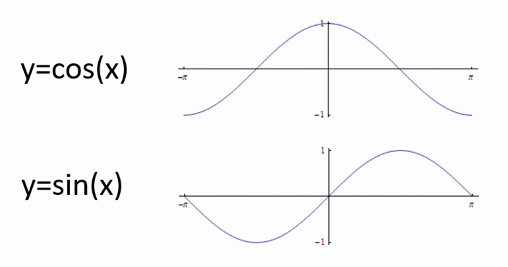
\includegraphics[width=0.7\textwidth]{sin_cos.PNG}} \end{center}

Other examples of even functions are $x^2$, $x^4$,  or any $x^n$ with $n$ an even number. Any constant multiple of an even function is even, e.g. $17x^4$.  You can take sum or difference of even functions and you get an even function, e.g. $x^2+x^4$, $x^8 - 17x^4 $.

Other examples of odd functions are $x^3$, $x^5$,  or any $x^n$ with $n$ an odd number. Any constant multiple of an odd function is even, e.g. $16x^3$.  You can take sum or difference of odd functions and you get an odd function, e.g. $x^3+x$, $x - 16x^3 $.

Most functions are neither even nor odd. $y= \ln x$, $y = e^x$ , and $y= x^2+6x+7$ are all examples of functions which are neither symmetric with respect to the y-axis nor the origin.

If you multiply an odd function with an even function, you get an odd function. This can be easily seen if you consider the example $x^3 \cdot x^2 = x^5 $. In similar fashion, you can see that multiplying two odd functions or multiplying two even functions will give you an even function.

Why are even or odd important? It is because of the following observations:

\begin{itemize}
\item  \textit{Integrating an odd function over a symmetric domain gives you zero}. In other words, if $f(x)$ is an odd function, then
$$\int_{-a}^{a} f(x) dx =0$$
In the above integral, the interval $[-a,a]$ is symmetric over the origin, so we say it's a symmetric domain. (On the other hand $[-2,10]$ would be an example of a domain that is not symmetric.)

\item  If you integrate an even function over a symmetric domain, you can simplify the calculation by doubling the integral over the half of the domain, i.e.
$$\int_{-a}^{a} f(x) dx = 2 \int_{0}^{a} f(x) dx $$
if $f(x)$ is an even function.
\end{itemize}
	
\subsection*{Orthogonality relations}

Since $\sin nx$ is an odd function and $\cos mx$ is an even function for $n$ and $m$ positive integers, their product is an odd function. Which means:
$$\int_{-\pi}^{\pi} \sin nx \cos mx dx = 0$$

In the previous sections, we have proved that:
$$\int_{-\pi}^{\pi} \sin nx \sin mx dx = \begin{cases} 0, \; \mathrm{ if } n \neq m \\ \pi, \; \mathrm{ if } n = m \end{cases} $$

Likewise one can prove the following:
$$\int_{-\pi}^{\pi} \cos nx \cos mx dx = \begin{cases} 0, \; \mathrm{ if } n \neq m \\ \pi, \; \mathrm{ if } n = m \end{cases} $$
You just have to use the identity $\cos A \cdot \cos B = \frac{1}{2} \left( \cos (A+B) + \cos (A-B) \right)$ to prove the above.

These integral results are called orthogonality relations.

One more formula that we will use frequently when computing Fourier Series is the following:
$$\sin n \pi =0$$
$$\cos n \pi = (-1)^n$$
You should draw the graph of sine and cosine to convince yourself that indeed sine is zero at multiples of $\pi$ while cosine alternates between 1 and -1 at multiples of $\pi$.

\subsection*{What is a Fourier Series?}

Fourier Series is a way to approximate a function by sums of sines and/or cosines. For example the following picture shows how cosine functions can be added together to immitate the function $y=x^2$:
\begin{center} \makebox[\textwidth]{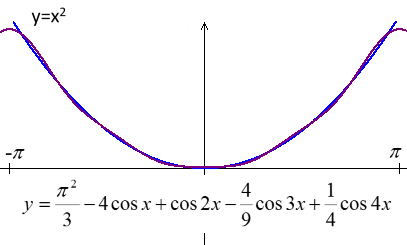
\includegraphics[scale=0.8]{x_squared.PNG}} \end{center}

Here is another example. This time, sum of some sine functions are trying to mimick a step function:
\begin{center} \makebox[\textwidth]{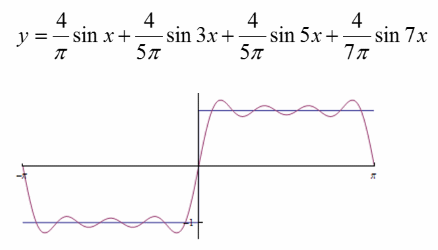
\includegraphics[width=0.7\textwidth]{stepfunc1.PNG}} \end{center}

Not impressed? Well, if we add more sine functions, the result is more convincing:
\begin{center} \makebox[\textwidth]{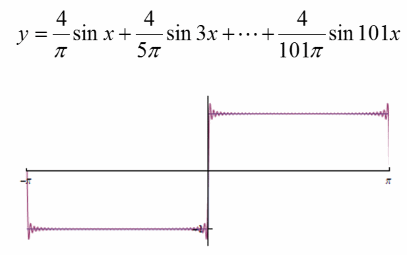
\includegraphics[width=0.7\textwidth]{stepfunc2.PNG}} \end{center}

Now all this begs the question: "How can we figure out the coefficients of these sine or cosine functions used above?"

Let's take a look at the function $y=x^2$ and try to figure out its Fourier series from scratch.

First thing to do is to try to represent $x^2$ as a sum of sine or cosine functions, i.e.:
$$x^2 = (a_0 + a_1 \cos x + a_2 \cos 2x + a_3 \cos 3x  + \cdots) + (b_1 \sin x + b_2 \sin 2x + b_3 \sin 3x + \cdots)$$

Now, $x^2$ is an even function, so it can only be sum of even functions. So all those sine functions shouldn't be there, or another way to say it will be that $b_n$ will be zero for all $n$. Therefore we have:
$$x^2 = a_0 + a_1 \cos x + a_2 \cos 2x + a_3 \cos 3x  + \cdots $$

Then let's integrate both sides over $[-\pi, \pi]$.
$$\int_{-\pi}^{\pi} x^2 dx = \int_{-\pi}^{\pi} a_0 + a_1 \cos x + a_2 \cos 2x + a_3 \cos 3x  + \cdots  dx $$

Using
$$\int_{-\pi}^{\pi} \cos nx dx = \frac{1}{n} (\sin n \pi - \sin -n \pi) =\frac{1}{n} (0-0) = 0,$$
we see that most of the integral of the right side is zero except for $\int_{-\pi}^{\pi} a_0 dx = a_0 \cdot 2\pi $

On the other hand, the left side is:
$$\int_{-\pi}^{\pi} x^2 dx = 2 \int_{0}^{\pi} x^2 dx = 2\cdot \frac{1}{3} \left( \pi^3 - 0^3 \right) = \frac{2\pi^3}{3} $$

So setting both sides equal gives us:
$$\frac{2\pi^3}{3} =a_0 \cdot 2\pi$$
$$a_0 = \frac{2\pi^3}{3} \cdot \frac{1}{2\pi} = \frac{\pi^2}{3}$$

Look at what we have! We found what $a_0$ is!

\textit{Now comes the ingenuous part.} We multiply $\cos x $ both sides:
$$x^2 \cos x = a_0 \cos x + a_1 \cos x \cos x + a_2 \cos 2x \cos x + a_3 \cos 3x \cos x + \cdots $$
and integrate it over $[-\pi, \pi]$. Good thing that we already have these integrals calculated, in the form the orthogonality relations:
$$\int_{-\pi}^{\pi} \cos nx \cos mx dx = \begin{cases} 0, \; \mathrm{ if } n \neq m \\ \pi, \; \mathrm{ if } n = m \end{cases} $$

In other words, if we integrate:
$$\int_{-\pi}^{\pi} x^2 \cos x dx = \int_{-\pi}^{\pi} a_0 \cos x + a_1 \cos x \cos x + a_2 \cos 2x \cos x + a_3 \cos 3x \cos x + \cdots  dx, $$
the right side involves integrals like $\int_{-\pi}^{\pi} a_2 \cos 2x \cos x dx$, which according to the orthogonality relations, is zero. The only term that is not zero on the right is:
$$\int_{-\pi}^{\pi} a_1 \cos x \cos x dx = a_1 \int_{-\pi}^{\pi} \cos x \cos x dx = a_1 \pi $$
On the other hand, the integral on the left side can be done via integral by parts (or tabular integration), to get:
$$\int_{-\pi}^{\pi} x^2 \cos x dx = 2\int_{0}^{\pi} x^2 \cos x dx = 2 \left. \left(x^2 \sin x + 2x \cos x - 2 \sin x \right) \right\vert_{0}^{\pi} = -4\pi$$

Hence setting both sides equal, we get:
$$-4 \pi = a_1 \pi $$
$$a_1 = -4 $$

We've only done this for $a_0$ and $a_1$, but the rest is same.

\subsection*{Formula for Fourier Series over  $[-\pi, \pi]$}

Say that we are given a function $f(x)$. Finding the Fourier Series of $f(x)$ means to express $f(x)$ as:
$$f(x) = (\frac{a_0}{2} + a_1 \cos x + a_2 \cos 2x + a_3 \cos 3x  + \cdots) + (b_1 \sin x + b_2 \sin 2x + b_3 \sin 3x + \cdots)$$

Written using the $\sum$ notation, this is:
$$f(x) = \frac{a_0}{2} +\sum_{n=0}^{\infty} \left( a_n \cos nx + b_n \sin nx \right) $$

(Notice the denominator 2 under $a_0$. This change will be explained in a moment.)
Just like the Taylor series approximation, if you truncate the right side, you get an approximation of the function $f(x)$, and the more terms you include on the right side, the better the approximation is. The only exception to this are points where the function $f(x)$ is not continuous. There is a mathematical theorem which proves that if the right side is taken to be the infinite series, the two sides will be equal everywhere except at points of jump discontinuity and also possibly at the endpoints of the interval ($-\pi$ and $\pi$ in our case). So this is the way the equal sign of the above formula should be understood. (The mathematically elaborate terminology for this is \textit{equal almost everywhere} or \textit{equal in $L_2$ sense.})

As we have seen before, multiplying $\cos nx$ both sides and integrating both sides over the interval $[-\pi, \pi]$ enables one to find $a_n$. Going through this process, one can find the formula:
$$a_n = \frac{1}{\pi} \int_{-\pi}^{\pi} f(x) \cos nx dx$$
Now, $a_0$ is slightly different because we don't have to multiply anything. However, since $\cos 0x = \cos 0 = 1$, we may still use the above formula for $a_0$. The reason there is the denominator 2 under $a_0$ is to make the above formula work for $n=0$. (If you want to know why, look back on the previous calculation done on $x^2$ and see that when $a_0$ was calculated, we had to divide by $2\pi$.)

Here is the formula for $b_n$ :
$$b_n = \frac{1}{\pi} \int_{-\pi}^{\pi} f(x) \sin nx dx$$

The formula is obtained in the same manner, with only difference being multiplying $\sin nx$ instead of $\cos nx$.

\subsection*{Integrals using orthogonality relations}

\begin{ex} Calculate the integral using orthogonality relations:
$$ \int_{-\pi}^{\pi} 4 \cos 3x \left( 3 \sin x + 4x + 5x^3 -10 \cos 3x + 2 \cos 8x \right) dx $$
\end{ex}

Solution) Recall that the orthogonality relations are:
$$\int_{-\pi}^{\pi} \sin nx \cos mx dx = 0$$
$$\int_{-\pi}^{\pi} \sin nx \sin mx dx = \begin{cases} 0, \; \mathrm{ if } n \neq m \\ \pi, \; \mathrm{ if } n = m \end{cases} $$
$$\int_{-\pi}^{\pi} \cos nx \cos mx dx = \begin{cases} 0, \; \mathrm{ if } n \neq m \\ \pi, \; \mathrm{ if } n = m \end{cases} $$

The above integral can be split as follows:
$$ =\int_{-\pi}^{\pi} 4 \cos 3x \cdot 3 \sin x + 4 \cos 3x \cdot 4x + 4 \cos 3x \cdot 5x^3$$
$$ \; \; \; \; \; \; \; \; -4 \cos 3x \cdot 10 \cos 3x + 4 \cos 3x \cdot 2 \cos 8x  dx $$
$$ = \int_{-\pi}^{\pi} 12 \cos 3x \sin x dx +\int_{-\pi}^{\pi} 16 x \cos 3x dx +\int_{-\pi}^{\pi} 20 x^3 \cos 3x dx $$
$$ \; \; \; \; \; \; \; \; +\int_{-\pi}^{\pi} -40 \cos 3x \cos 3x  dx +\int_{-\pi}^{\pi} 8 \cos 3x \cos 8x dx $$

From orthogonality relations, we know that $\int_{-\pi}^{\pi} 12 \cos 3x \sin x dx = 12 \int_{-\pi}^{\pi} \cos 3x \sin 1x dx =0$ and $\int_{-\pi}^{\pi} 8 \cos 3x \cos 8x dx =0 $, while
$\int_{-\pi}^{\pi} -40 \cos 3x \cos 3x  dx =-40 \int_{-\pi}^{\pi} \cos 3x \cos 3x  dx =-40\pi$.

For $\int_{-\pi}^{\pi} 16 x \cos 3x dx$, we know that $16x$ is an \textit{odd function} while $\cos 3x$ is an even function. Thus the product is odd and since it is integrated over the \textit{symmetric domain} $[-\pi, \pi]$, the integral is zero. $\int_{-\pi}^{\pi} 20 x^3 \cos 3x dx $ is zero for the same reason.

Therefore, we found that all the integrals are zero except the one where $\cos 3x$ is multiplied by itself. In that case the answer is:
$$\int_{-\pi}^{\pi} -40 \cos 3x \cos 3x  dx =-40 \int_{-\pi}^{\pi} \cos 3x \cos 3x  dx =-40\pi$$

\subsection*{Calculating Fourier series over  $[-\pi, \pi]$}

\begin{ex} Find the Fourier series of the function $f(x) = x^2 -3x$ defined over the interval $[-\pi, \pi]$.
\end{ex}
The Fourier Series of the function is
$$f(x) = \frac{a_0}{2} + \sum_{n=1}^{\infty} \left( a_n \cos nx + b_n \sin nx \right) $$

What we have to do is to find $a_0$, $a_n$ and $b_n$.

\textbf{step 1} Find $a_0$.
$$a_0 = \frac{1}{\pi} \int_{-\pi}^{\pi} f(x) \cos 0x dx$$
$$= \frac{1}{\pi} \int_{-\pi}^{\pi} f(x)dx = \frac{1}{\pi} \int_{-\pi}^{\pi} x^2 -3x dx$$
$$= \frac{2}{\pi} \int_{0}^{\pi} x^2 dx$$
$$= \left. \frac{2}{3\pi} x^3 \right\vert_0^{\pi}$$
$$= \frac{2 \pi^2}{3}$$
In the above calculation, we used the fact that $-3x$ is an odd function where as $x^2$ is an even function.

\textbf{step2} Find $a_n$
$$a_n = \frac{1}{\pi} \int_{-\pi}^{\pi} f(x) \cos nx dx$$
$$= \frac{1}{\pi} \int_{-\pi}^{\pi} (x^2 -3x) \cos nx dx$$
Now, using the fact that even function times even function is an even function and also that odd function times odd function is odd, we see that the above is equal to:
$$ = \frac{2}{\pi} \int_{0}^{\pi} x^2 \cos nx dx$$
Then using the integration by parts, we have:
$$= \frac{2}{\pi} \left. \left(\frac{x^2}{n} \sin nx + \frac{2x}{n^2} \cos nx - \frac{2}{n^3} \sin nx \right) \right\vert_{0}^{\pi} = \frac{4}{n^2} (-1)^n $$

\textbf{step 3} Find $b_n$
$$b_n = \frac{1}{\pi} \int_{-\pi}^{\pi} f(x) \sin nx dx$$
$$ =\frac{2}{\pi} \int_{0}^{\pi} -3x \sin nx dx $$
(Note: $x^2 \sin nx$ is an odd function, and so its integral will be zero.)
By integration by parts, we have:
$$ =-\frac{2}{\pi} \left. \left(\frac{-3x}{n} \cos nx + \frac{-3}{n^2} \sin nx \right) \right\vert_{0}^{\pi} = \frac{6}{n} (-1)^n $$

\textbf{step 4} Put everything into the series:
$$x^2-3x = \frac{\pi^2}{3}+\sum_{n=1}^{\infty} \left( \frac{4}{n^2} (-1)^n \cos nx + \frac{6}{n} (-1)^n \sin nx \right) $$

That's how it's done!

\subsection*{Fourier Series over  $[-L, L]$ }

One problem of the Fourier series so far is that it is only defined on the interval $[-\pi, \pi]$. This means that the Fourier series will only approximate the given function on the interval $[-\pi, \pi]$. In order for Fourier series to be useful, one has to modify it so that it can work on any arbitrary interval $[-L, L]$. (Or any interval $[A,B]$. However, usually people use Fourier series on $[-L, L]$ or $[0,L]$. The formulas to use for the case $[0,L]$ is written in the appendix.)

Let's review what the Fourier series looks like on $[-\pi, \pi]$.

$$f(x) = \frac{a_0}{2} +\sum_{n=0}^{\infty} \left( a_n \cos nx + b_n \sin nx \right) $$

The right side of the above equation has the interval $[-\pi,\pi]$ as one period. The reason for this is that when $n=1$, the summation produces $a_1 \cos 1\cdot x + b_1 \sin 1\cdot x$ and both $\cos x$ and $\sin x$ have $2\pi$ as one period. Then the $n=2$ produces $a_2 \cos 2x + b_2 \sin 2x $ and $\cos 2x$ and $\sin 2x$ have $\pi$ as one period. In fact for any $n$,  $\cos nx$ and $\sin nx$ have period $\frac{2\pi}{n}$. This means that in the interval $[-\pi,\pi]$, some integer multiples of periods of these trigonometric functions fit exactly. Adding such functions will give us a function that has period of $2\pi$. To explain why, think about a combination of events that repeat every week and events that repeat every day and events that repeat every hour. Then every week will have the same schedule and the combination of all events will have a period of one week (i.e. every week will be a repeat of the previous week.)

Now, notice that the formulas for $a_n$ and $b_n$ are
$$a_n = \frac{1}{\pi} \int_{-\pi}^{\pi} f(x) \cos nx dx$$
$$b_n = \frac{1}{\pi} \int_{-\pi}^{\pi} f(x) \sin nx dx$$
which only makes use of the value of the function $f(x)$ on the interval $[-\pi,\pi]$. Thus when you have a function $f(x)$, not necessarily periodic with period $2\pi$, then the Fourier Series
$$f(x) = \frac{a_0}{2} +\sum_{n=0}^{\infty} \left( a_n \cos nx + b_n \sin nx \right) $$
are meant to hold only true on the interval $[-\pi,\pi]$. Here is another way to think about this. Since the right side is periodic with period $2\pi$, \textit{the Fourier series takes a function's value on the interval $[-\pi,\pi]$ and makes a period extension of this restricted function.}

All this observation can now be used to come up with a formula for the Fourier series on the interval $[-L, L]$. First, we introduce $L$ into the formula  $\cos \frac{n \pi x}{L}$ and $\sin \frac{n\pi x}{L}$ so that these functions will have integer multiple periods that fit exactly in the interval $[-L, L]$.

The result is 
$$f(x) = \frac{a_0}{2} +\sum_{n=0}^{\infty} \left( a_n \cos \frac{n \pi x}{L} + b_n \sin \frac{n\pi x}{L} \right) $$
and the integrals for finding the coefficients are also changed accordingly:
$$a_n = \frac{1}{L} \int_{-L}^{L} f(x) \cos \frac{n\pi x }{L} dx$$
$$b_n = \frac{1}{L} \int_{-L}^{L} f(x) \sin \frac{n\pi x }{L} dx$$ 

The $\frac{1}{L}$ factor is introduced because the orthogonality relations are 
$$\int_{-L}^{L} \cos \frac{n\pi x}{L} \cos \frac{m\pi x }{L}  = \begin{cases} 0, \; \mathrm{ if } n \neq m \\ L, \; \mathrm{ if } n = m \end{cases} $$
and 
$$\int_{-L}^{L} \sin \frac{n\pi x}{L}  \sin \frac{m\pi x}{L}  = \begin{cases} 0, \; \mathrm{ if } n \neq m \\ L, \; \mathrm{ if } n = m \end{cases} $$
which I leave the reader to check. You should also check that the Fourier series is exactly same as the previous one if you set $L=\pi$, just as it should.

\subsection*{Calculation of Fourier Series}

\begin{ex}
	Find the Fourier series of 
	\end{ex}
	$$f(x) = |x| +2x \; \; \textrm{on } \; \; [-3,3]$$

Solution)
Before we calculate, note that the interval given is $[-3,3]$, so that $L=3$. Also note that $|x|$ is an even function and $2x$ is an odd function. Thus when integrating with the odd function $\sin \frac{m\pi}{3} x$, the even part $|x|$ will yield zero while when integrating with the even function $\cos \frac{m\pi}{3} x$, the odd part $2x$ will yield zero. We compute the integrals as follows.
$$a_0 = \frac{1}{3} \int_{-3}^{3} (|x| +2x) \cos \frac{0\cdot \pi x }{3} dx = \frac{1}{3} \int_{-3}^{3} (|x| +2x) \cdot 1 dx $$
$$= \frac{1}{3} \int_{-3}^{3} |x| dx = \frac{2}{3} \int_{0}^{3} x dx = \frac{2}{3} \left. \left( \frac{1}{2} x^2 \right) \right\vert_0^3 = 3 $$
Then for $a_n$ and $b_n$ we need to perform integration by parts (or tabular integration) to get:
$$a_n = \frac{1}{3} \int_{-3}^{3} (|x| +2x) \cos \frac{n\pi x }{3} dx = \frac{1}{3} \int_{-3}^{3} |x| \cos \frac{n \pi x }{3} dx = \frac{2}{3} \int_{0}^{3} x \cos \frac{n\pi x }{3} dx$$
$$= \frac{2}{3} \left. \left( \frac{3}{n\pi} x \sin \frac{n\pi x }{3} + \frac{9}{n^2\pi^2} \cos \frac{n\pi x }{3} \right) \right\vert_0^3 = \frac{2}{3} \left(  \frac{9}{n\pi} \sin n\pi + \frac{9}{n^2\pi^2} \cos n\pi - \left(0 + \frac{9}{n^2\pi^2} \right) \right) $$
$$ = \frac{2}{3} \left( \frac{9}{n^2\pi^2} (-1)^n - \frac{9}{n^2\pi^2} \right) =\frac{6}{n^2\pi^2} \left((-1)^n-1\right) $$

$$b_n = \frac{1}{3} \int_{-3}^{3} (|x| +2x) \sin \frac{n\pi x }{3} dx = \frac{1}{3} \int_{-3}^{3} 2 x \sin \frac{n \pi x }{3} dx = \frac{2}{3} \int_{0}^{3} 2x \sin \frac{n\pi x }{3} dx$$
$$= \frac{2}{3} \left. \left( - \frac{6}{n\pi} x \cos \frac{n\pi x }{3} + \frac{18}{n^2\pi^2} \sin \frac{n\pi x }{3} \right) \right\vert_0^3 = \frac{2}{3} \left(  -\frac{18}{n\pi} \cos n\pi + \frac{18}{n^2\pi^2} \sin n\pi - \left(-\frac{18}{n\pi} + 0 \right) \right) $$
$$ = \frac{2}{3} \left( -\frac{18}{n\pi} (-1)^n +\frac{18}{n\pi} \right) = \frac{18}{n\pi} \left(-(-1)^n+1\right) $$

Therefore the answer is:
$$|x| +2x = \frac{3}{2} +\sum_{n=0}^{\infty} \left( \frac{6}{n^2\pi^2} \left((-1)^n-1\right)  \cos \frac{n \pi x}{3} + \frac{18}{n\pi} \left(-(-1)^n+1\right) \sin \frac{n\pi x}{3} \right) $$
where the left and right side agree (except for a few points) on the interval $[-3,3]$.

\subsection*{Fourier series of a piecewise function}

\begin{ex}
	Find the Fourier series of 
\end{ex}
	$$f(x) = \begin{cases} -2, \; \mathrm{ if } -5<x<0 \\ 2 , \; \mathrm{ if } 0\leq x \leq 5 \end{cases} $$

Solution)
The graph is almost same as
\begin{center} \makebox[\textwidth]{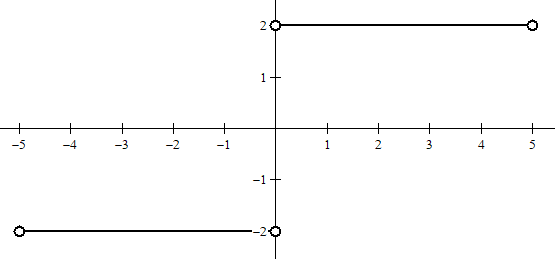
\includegraphics[width=0.6\textwidth]{piecewise_fourier.PNG}} \end{center}
except for the fact that the two open circles of the bottom line should be closed. However, Fourier series only gives equality away from jump discontinuity and also possibly away from the end points, it doesn't matter whether we are looking for Fourier series with the closed circle or the open circle. 

Note that this function is an odd function. Therefore we know that $a_n$'s vanish. So we will only compute $b_n$.

$$b_n = \frac{1}{5} \int_{-5}^{5} f(x) \sin \frac{n\pi x }{5} dx = \frac{1}{5} \int_{-5}^{0} (-2) \sin \frac{n\pi x }{5} dx + \frac{1}{5} \int_{0}^{5} 2 \sin \frac{n\pi x }{5} dx$$
$$= \frac{1}{5} \left. \frac{10}{n\pi} \cos \frac{n\pi x }{5} \right\vert_{-5}^0 + \frac{1}{5} \left. \left(-\frac{10}{n\pi} \cos \frac{n\pi x }{5} \right) \right\vert_{0}^5 $$
$$= \frac{2}{n\pi} - \frac{2}{n\pi} (-1)^n + \left(- \frac{2}{n\pi} (-1)^n +\frac{2}{n\pi} \right) = \frac{4}{n\pi} \left(1-(-1)^n\right)$$

Therefore the answer is:
$$f(x) = \sum_{n=0}^{\infty}  \frac{4}{n\pi} \left( 1-(-1)^n \right) \sin \frac{n\pi x}{5} $$

Note that we could have simplified the calculation by just using the fact that $f(x) sin \frac{n\pi x }{5}$ is an even function and therefore we can just double the integration on the half interval $[0,5]$. However, the above integration was performed to demonstrate how to deal with piecewise functions. 



\section{Fourier Sine Series and Cosine Series}

\subsection*{Even and Odd extension of a function }

\begin{ex} Find the even extension of the function $f(x)= x$ which is defined on $[0,4]$.
	\end{ex}
Solution)
Consider the graph of the function:
\begin{center} \makebox[\textwidth]{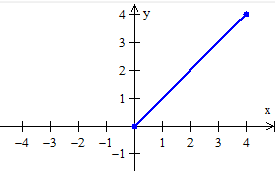
\includegraphics[scale=0.8]{x_on_0_4.PNG}} \end{center}

An even function is symmetric with respect to the y-axis, so if the function is extended as an even function, its graph would be:
\begin{center} \makebox[\textwidth]{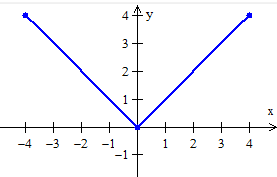
\includegraphics[scale=0.8]{abs_x.PNG}} \end{center}

As you can see, the newly added left part is a straight line whose slope is (-1) and whose y-intercept is zero. So it is easy to see that the function on the left is $-x$.

Thus we conclude that the extended function is a piecewise function whose formula is given as:
$$f(x) = \begin{cases} x \; , \; \; 0\leq x\leq 4 \\ -x  \; , \; \; -4 \leq x < 0 \end{cases} $$

\subsection*{Formula for even extensions}

A way to define an even function without using the graph, is to simply say that it is a function that satisfies $f(x)=f(-x)$. In other words, even functions are functions that give you the same value whether you plug in a positive or negative of the same number. One can check that if a function $f(x)$ is defined on the interval $[0,L]$, the piecewise function:
$$f(x) = \begin{cases} f(x)  \; , \; \;  0\leq x\leq L \\ f(-x)  \; , \; \; -L \leq x < 0 \end{cases} $$
satisfies the requirement $f(x)=f(-x)$. Check that this formula indeed gives you the same answer for the example in the beginning. Let's apply this to a second example:

\begin{ex} $f(x) = e^x$ on $[0,3]$. What is the even extension?
	\end{ex}
Answer:
$$f(x) = \begin{cases} e^x  \; , \; \;  0\leq x\leq 3 \\ e^{-x}  \; , \; \; -3 \leq x < 0 \end{cases} $$

\subsection*{Odd extension}
A function is odd if it satisfies $f(x)=-f(-x)$. If a function $f(x)$ is defined on the interval $[0,L]$, you can extend it to an odd function by formula:
$$f(x) = \begin{cases} f(x)  \; , \; \;  0\leq x\leq L \\ -f(-x)  \; , \; \; -L \leq x < 0 \end{cases} $$

\begin{ex} $f(x) = e^x$ on $[0,3]$. What is the odd extension?
	\end{ex}
Answer:
$$f(x) = \begin{cases} e^x  \; , \; \;  0\leq x\leq 3 \\ -e^{-x}  \; , \; \; -3 \leq x < 0 \end{cases} $$

There is a slight problem with this answer. If you draw the graph it is not symmetric with respect to the origin because there is an open circle at (0,-1) while a solid circle is at (0,1). But since we are mostly using even or odd functions in the context of integration, the fact that the value of a function at one point doesn't affect the integrals makes it a non-issue. If you want a perfect odd symmetry, you should use:
$f(x) = \begin{cases} f(x)  \; , \; \;  0< x\leq L \\ 0 \; , \; \; x=0 \\ -f(-x)  \; , \; \; -L \leq x < 0 \end{cases} $
Note that this function agrees with the original function $f(x)$ on $(0, L]$ but may not agree at $x=0$.



\subsection*{Introduction to Fourier sine series and Fourier cosine series}

So far we have learned the Fourier Series of the function as :
$$f(x) = \frac{a_0}{2} + \sum_{n=1}^{\infty} \left( a_n \cos \frac{n\pi}{L} x + b_n \sin \frac{n\pi}{L} x \right) $$
where the coefficients are obtained by:
$$a_n = \frac{1}{L} \int_{-L}^{L} f(x) \cos \frac{n\pi}{L} x dx$$
$$b_n = \frac{1}{L} \int_{-L}^{L} f(x) \sin \frac{n\pi}{L} x dx$$

If $f(x)$ is an even function, then the $\sin$ terms (being odd functions) won't be there and you'll only get the $\cos$ terms, i.e.:
$$f(x) = \frac{a_0}{2} + \sum_{n=1}^{\infty}  a_n \cos \frac{n\pi}{L} x  $$
where the coefficients are obtained by:
$$a_n = \frac{2}{L} \int_{0}^{L} f(x) \cos \frac{n\pi}{L} x dx$$
Note that in the above formula for $a_n$, we are using the fact that $f(x)\cos \frac{n\pi}{L} x$ is even, to take the double value of integration to be on $[0,L]$.

If $f(x)$ is an odd function, then the $\cos$ terms and also the $\frac{a_0}{2}$ term (being even functions) won't be there and you'll only get the $\sin$ terms, i.e.:
$$f(x) = \sum_{n=1}^{\infty}  b_n \sin \frac{n\pi}{L} x  $$
where the coefficients are obtained by:
$$b_n = \frac{2}{L} \int_{0}^{L} f(x) \sin \frac{n\pi}{L} x dx$$
Note that in the above formula for $b_n$, we are using the fact that $f(x)\sin \frac{n\pi}{L} x$ is even, to take the double value of integration to be on $[0,L]$.

\subsection*{Definition of Fourier sine series and Fourier cosine series}

Suppose a function $f(x)$ is given on the interval $[0,L]$. Then we may make an even extension or an odd extension of the function to make it a function over the interval $[-L,L]$.

A \textit{Fourier cosine series} of a function is the Fourier series of the \textit{even extension of the function}.

A \textit{Fourier sine series} of a function is the Fourier series of the \textit{odd extension of the function}.

\begin{ex} Find Fourier cosine series of $f(x) = x+2$ on $[0,5]$.
	\end{ex}
Solution)
Since we are taking even extension, we are to use:
$$f(x) = \frac{a_0}{2} + \sum_{n=1}^{\infty}  a_n \cos \frac{n\pi}{L} x  $$
where the coefficients are obtained by:
$$a_n = \frac{2}{L} \int_{0}^{L} f(x) \cos \frac{n\pi}{L} x dx$$

We calculate:
$$a_0 = \frac{2}{5} \int_0^5 (x+2) dx = \frac{2}{5} \left(\frac{1}{2} x^2 + 2x \right) \Bigg\vert_0^5 = 9$$
and then
$$a_n = \frac{2}{5} \int_0^5 (x+2) \cos \left(\frac{n\pi x}{5} \right) dx $$
$$ = \frac{2}{5} \left((x+2)\cdot \frac{5}{n\pi} \sin \left(\frac{n\pi x}{5} \right) + \left(\frac{5}{n\pi} \right)^2 \cos \left(\frac{n\pi x}{5} \right) \right) \Bigg\vert_0^5$$
$$ = \frac{10}{n^2\pi^2} \left( (-1)^n -1 \right)$$

As done above, \textit{it is important to find } $a_0$ \textit{separately}. Also once you get the coefficients, you should write down the sum for the final answer:

$$f(x) = \frac{9}{2} + \sum_{n=1}^{\infty}  \frac{10}{n^2\pi^2} \left( (-1)^n -1 \right) \cos \frac{n\pi}{5} x  $$



\subsection*{Fourier Sine series example }
\begin{ex} Find Fourier sine series of $f(x) = x+2$ on $[0,5]$.
	\end{ex}
Solution)
Since we are taking odd extension, we are to use:
$$f(x) = \sum_{n=1}^{\infty}  b_n \sin \frac{n\pi}{L} x  $$
where the coefficients are obtained by:
$$b_n = \frac{2}{L} \int_{0}^{L} f(x) \sin \frac{n\pi x}{L}  dx$$

So we calculate:
$$b_n = \frac{2}{5} \int_0^5 (x+2) \sin \left(\frac{n\pi x}{5} \right) dx $$
$$ = \frac{2}{5} \left(-(x+2)\cdot \frac{5}{n\pi} \cos \left(\frac{n\pi x}{5} \right) + \left(\frac{5}{n\pi} \right)^2 \sin \left(\frac{n\pi x}{5} \right) \right) \Bigg\vert_0^5$$
$$ = \frac{2}{n\pi} \left( 2 -7\cdot (-1)^n  \right)$$

Notice that for sine series we do not have to calculate $a_0$ separately. Thus the answer is:
$$f(x) = \sum_{n=1}^{\infty}  \frac{2}{n\pi} \left( 2 -7\cdot (-1)^n  \right) \sin \frac{n\pi}{5} x $$

\subsection*{Fourier cosine series example }

\begin{ex}
	Find the Fourier cosine series of
\end{ex}
$$f(x) = 2x+1 \; \; \textrm{ on } \; [0,4]$$

Solution)
Since we are taking an even extension, we are to use:
$$f(x) = \frac{a_0}{2} \sum_{n=1}^{\infty}  a_n \cos \frac{n\pi}{L} x  $$
where the coefficients are obtained by:
$$a_n = \frac{2}{L} \int_{0}^{L} f(x) \cos \frac{n\pi x}{L}  dx$$

So we calculate:
$$a_0 =  \frac{2}{4} \int_{0}^{4} 2x+1 dx = \frac{2}{4} (x^2+x)\Big|_0^4 = 10$$

$$a_n = \frac{2}{4} \int_{0}^{4} (2x+1) \cos \frac{n\pi x}{4}  dx = \frac{2}{4} \left( \frac{4}{n\pi} (2x+1) \sin \frac{n\pi x}{4} + \frac{32}{n^2\pi^2} \cos \frac{n\pi x}{4} \right) \Big\vert_0^4 $$
$$ = \frac{16}{n^2\pi^2} \left( (-1)^n -1 \right) $$

Thus the answer is:

$$2x+1 = 5+ \sum_{n=1}^{\infty}  \frac{16}{n^2\pi^2} \left( (-1)^n -1 \right) \cos \frac{n\pi}{4} x  $$
which holds true on the interval $[0,4]$.

\subsection*{Fourier cosine series of a piecewise function }
A superior property of the Fourier series over the Taylor series is that it can be used to find approximations for functions that are not continuous. So let us try the following example.

\begin{ex} Find the Fourier cosine series of:
$$ f(x) = \begin{cases} 3 \; , \; \; 0 < x \leq 2 \\ x+1  \; , \; \;  2< x \leq 4 \\ \end{cases} $$
\end{ex}
Solution)
Since the function is defined on the interval $(0,4]$, we have $L=4$.
When computing the integral of a piecewise function, it is necessary to split the integral.
$$a_0 = \frac{2}{4} \int_0^4 f(x) dx = \frac{1}{2} \left( \int_0^2 f(x) dx + \int_2^4 f(x) dx \right)$$
$$ = \frac{1}{2} \int_0^2 3 dx +\frac{1}{2} \int_2^4 x+1 dx $$
$$ = \frac{3}{2}x \Bigg\vert_0^2 +  \left(\frac{1}{4} x^2 + \frac{1}{2} x \right)\Bigg\vert_2^4 = 7$$

$$a_n = \frac{2}{4} \int_0^4 f(x) \cos \left(\frac{n\pi x}{4} \right) dx = \frac{1}{2} \int_0^2 f(x) \cos \left(\frac{n\pi x}{4} \right) dx +\frac{1}{2} \int_2^4 f(x) \cos \left(\frac{n\pi x}{4} \right) dx$$

The first integral is:
$$ \frac{1}{2} \int_0^2 3 \cos \left(\frac{n\pi x}{4} \right) dx = \frac{1}{2} \cdot 3 \cdot \frac{4}{n\pi} \sin \left(\frac{n\pi x}{4} \right) \Bigg\vert_0^2 $$
$$ = \frac{6}{n\pi} \sin \frac{n\pi}{2} $$

The second integral is:
$$\frac{1}{2} \int_2^4 (x+1) \cos \left(\frac{n\pi x}{4} \right) dx$$
$$ =\frac{1}{2} \left( (x+1) \cdot \frac{4}{n\pi} \sin \left(\frac{n\pi x}{4} \right) +\frac{16}{n^2\pi^2} \cos \left(\frac{n\pi x}{4} \right) \right) \Bigg\vert_2^4 $$
$$ = -\frac{6}{n\pi} \sin \frac{n\pi}{2}+\frac{8}{n^2\pi^2} (-1)^n  - \frac{8}{n^2\pi^2} \cos \frac{n\pi}{2}$$

Adding the two we get:
$$a_n = \frac{6}{n\pi} \sin \frac{n\pi}{2} -\frac{6}{n\pi} \sin \frac{n\pi}{2}+\frac{8}{n^2\pi^2} (-1)^n  - \frac{8}{n^2\pi^2} \cos \frac{n\pi}{2}$$
$$= \frac{8}{n^2\pi^2} (-1)^n  - \frac{8}{n^2\pi^2} \cos \frac{n\pi}{2}$$

The $\cos \frac{n\pi}{2}$ takes the value of 1, 0 or -1. So we should investigate it in two cases. If $n$ is even, then $n=2m$ for some $m$, which makes $\cos \frac{n\pi}{2} = \cos(m\pi) =(-1)^m $. If $n$ is odd, then $\cos \frac{n\pi}{2}=0$ (You should draw the graph of $\cos$ in order to convince yourself.)

For each case we have:
\begin{itemize}
\item  Case $n=2m$
\end{itemize}
$$a_n = \frac{8}{n^2\pi^2} (-1)^n  - \frac{8}{n^2\pi^2} \cos \frac{n\pi}{2}$$
$$ = \frac{8}{(2m)^2\pi^2} (-1)^{2m}  - \frac{8}{(2m)^2\pi^2} (-1)^m $$
$$ = \frac{2}{m^2\pi^2} - \frac{2}{m^2\pi^2} (-1)^m $$
$$ = \frac{2}{m^2\pi^2} \left( 1 - (-1)^m \right) $$

\begin{itemize}
\item  Case $n=2m-1$ (i.e. $n$ is odd)
\end{itemize}
$$a_n = \frac{8}{n^2\pi^2} (-1)^n  - \frac{8}{n^2\pi^2} \cos \frac{n\pi}{2}$$
$$= \frac{8}{n^2\pi^2} (-1)^{2m-1} -0$$
$$ =  - \frac{8}{(2m-1)^2\pi^2}$$

Answer:
$$f(x) = \frac{7}{2} + \sum_{m=1}^{\infty} \Big[ - \frac{8}{(2m-1)^2\pi^2} \cos \frac{(2m-1)\pi x}{4} + \frac{2}{m^2\pi^2} \left( 1 - (-1)^m \right) \cos \frac{2m\pi x}{4} \Big]$$

Note: You can also simplify $\cos \frac{2m\pi x}{4}$ as $\cos \frac{m\pi x}{2}$

\subsection*{Fourier sine series of a piecewise function }

\begin{ex} Let
$$f(x) = \begin{cases} x  \; , \; \; 0\leq x \leq 1 \\ 1  \; , \; \; 1<x\leq 3 \end{cases}$$
Find the first three non-zero terms of the Fourier Sine Series.
\end{ex}

Solution)
Fourier sine series is
$$f(x) = \sum_{n=1}^{\infty}  b_n \sin \frac{n\pi}{L} x  $$
where the coefficients are obtained by:
$$b_n = \frac{2}{L} \int_{0}^{L} f(x) \sin \frac{n\pi}{L} x dx$$

In our case, since $f(x)$ is defined on $[0,3]$, we have $L=3$ and:
$$b_n = \frac{2}{3} \int_{0}^{3} f(x) \sin \frac{n\pi}{3} x dx = \frac{2}{3} \int_{0}^{1} f(x) \sin \frac{n\pi}{3} x dx +\frac{2}{3} \int_{1}^{3} f(x) \sin \frac{n\pi}{3} x dx $$
$$= \frac{2}{3} \int_{0}^{1} x \sin \frac{n\pi}{3} x dx +\frac{2}{3} \int_{1}^{3} 1 \cdot \sin \frac{n\pi}{3} x dx $$
$$ = \frac{2}{3} \left(-\frac{3}{n\pi} x \cos \frac{n\pi}{3} x + \frac{9}{n^2\pi^2}  \sin \frac{n\pi}{3} x \right) \Bigg\vert_0^1 + \frac{2}{3} \left(-\frac{3}{n\pi} \cos \frac{n\pi}{3} x \right) \Bigg\vert_1^3$$
$$= \left(-\frac{2}{n\pi} x \cos \frac{n\pi}{3} x + \frac{6}{n^2\pi^2}  \sin \frac{n\pi}{3} x \right) \Bigg\vert_0^1 +\left(-\frac{2}{n\pi} \cos \frac{n\pi}{3} x \right) \Bigg\vert_1^3$$
$$ = -\frac{2}{n\pi} \cos \frac{n\pi}{3} +\frac{6}{n^2\pi^2} \sin \frac{n\pi}{3} -0 -\frac{2}{n\pi} (-1)^n + \frac{2}{n\pi} \cos \frac{n\pi}{3}$$
$$ = \frac{6}{n^2\pi^2} \sin \frac{n\pi}{3} -\frac{2}{n\pi} (-1)^n$$

Since we are told to find 3 non-zero terms, we compute $b_1$, $b_2$ and $b_3$ using the above formula:
$$b_1 = \frac{6}{\pi^2} \sin \frac{\pi}{3} - \frac{2}{\pi}(-1)^1 = \frac{3\sqrt{3}}{\pi^2}+\frac{2}{\pi}$$
$$b_2=  \frac{6}{4\pi^2} \sin \frac{2\pi}{3} - \frac{2}{2\pi}(-1)^2 = \frac{3\sqrt{3}}{4\pi^2}-\frac{1}{\pi}$$
$$b_3 = 0 - \frac{2}{3\pi}(-1)^3= \frac{2}{3\pi}$$

Thus the first three non-zero terms of the sine series is:
$$f(x) = \left(\frac{3\sqrt{3}}{\pi^2}+\frac{2}{\pi} \right)\sin \frac{\pi}{3} x + \left( \frac{3\sqrt{3}}{4\pi^2}-\frac{1}{\pi} \right) \sin \frac{2\pi}{3} x + \frac{2}{3\pi}\sin \frac{3\pi}{3} x +\cdots$$

\subsection*{Solving Endpoint Value Problem using Fourier series }

\begin{ex}
$$y''+4y =t  \; , \; \; y(0)=y(2)=0$$
\end{ex}
Note: The conditions $y(0)=0$ and $y(2)=0$ are endpoint value conditions, and the differential equation $y''+4y =t$ is thought to hold for $0<t<2$ (i.e. in between the endpoints 0 and 2). The goal is to find a continuous function that satisfies both the differential equation and the endpoint conditions. Although this can be solved using the usual method of undetermined coefficients, let us learn how to find the solution using Fourier series. (The advantage of Fourier series solution is that the right side, $t$, could be replaced by any piecewise continuous function and we can still solve it.)

Solution) Notice that the trigonometric functions that satisfy $y(0)=0$ and $y(2)=0$ are $\sin$ functions of certain period. More specifically, $\sin \frac{2n\pi}{2} t $ satisfies the requirement. The idea of the solution is to put $y$ as sum of these functions, i.e.
$$y = \sum_{n=1}^{\infty} c_n \sin \frac{2n\pi}{2} t$$
Then it will automatically satisfy the endpoint value conditions. Let us differentiate in order to plug this into the differential equation.
$$y'' = \sum_{n=1}^{\infty} -\frac{n^2\pi^2}{4} c_n \sin \frac{2n\pi}{2} t$$

Plugging in, we have:
$$y''+ 4y = \sum_{n=1}^{\infty} -\frac{n^2\pi^2}{4} c_n \sin \frac{2n\pi}{2} t + 4\sum_{n=1}^{\infty}  c_n \sin \frac{2n\pi}{2} t $$
$$ = \sum_{n=1}^{\infty} \left(-\frac{n^2\pi^2}{4}+4 \right) c_n \sin \frac{2n\pi}{2} t $$

Now this has to be matched with the right side, which is $t$. But when you set them equal, the conclusion is not clear:
$$\sum_{n=1}^{\infty} \left(-\frac{n^2\pi^2}{4}+4 \right) c_n \sin \frac{2n\pi}{2} t =t$$
In other words, we can't figure out what $c_n$ should be. Thus we take the Fourier sine series of $t$.
$$ t = \sum_{n=1}^{\infty} b_n \sin \frac{2n\pi}{2} t$$
where
$$b_n = \frac{2}{2} \int_0^2 t \sin \frac{2n\pi}{2} t = \left( \frac{-2}{n\pi} t \cos \frac{2n\pi}{2} t + \frac{4}{n^2\pi^2} \sin  \frac{n\pi}{2} t \right) \Bigg\vert_0^2 $$
$$ = -\frac{4}{n\pi} (-1)^n$$
So we have:
$$ t = \sum_{n=1}^{\infty} -\frac{4}{n\pi} (-1)^n \sin \frac{2n\pi}{2} t$$
Now, since both sides look similar, we can compare the coefficients to deduce the following:
$$\sum_{n=1}^{\infty} \left(-\frac{n^2\pi^2}{4}+4 \right) c_n \sin \frac{2n\pi}{2} t =\sum_{n=1}^{\infty} -\frac{4}{n\pi} (-1)^n \sin \frac{2n\pi}{2} t$$
$$\left(-\frac{n^2\pi^2}{4}+4 \right) c_n = -\frac{4}{n\pi} (-1)^n$$
Solving this for $c_n$ gives us:
$$c_n = \frac{-\frac{4}{n\pi} (-1)^n}{-\frac{n^2\pi^2}{4}+4} $$

Plugging this back into $y$ gives us the answer:
$$y = \sum_{n=1}^{\infty} \frac{-\frac{4}{n\pi} (-1)^n}{-\frac{n^2\pi^2}{4}+4} \sin \frac{2n\pi}{2} t$$


\chapter{Partial Differential Equations}

\section{Heat Equation}

\subsection*{Introduction to heat equation }

Consider the following situation. A thin, long rod is inside some insulation with exposed ends, so that the only way heat can enter or escape is at the end points. Our goal is to figure out the temperature distribution $u(x,t)$ which means "temperature at point $x$ at time $t$". There is some initial temperature distribution at time $t=0$. Let's call it $u_0(x)$ so that $u(x,0)=u_0(x)$. (This condition is called the \textbf{initial condition \index{initial condition of PDE}}.) 
Also let the two endpoints touch ice so that the end points are always kept to 0 degree Celsius. If we denote $x=0$ for the position of the left end point and $x=L$ for the position of the right end point (which means that the length of the rod is $L$), then having temperature of zero at those points at all time $t$ means $u(0,t)=0$ and $u(L,t)=0$. (This condition is called the \textbf{boundary conditions \index{boundary condition}}.) Here is a picture to help you understand the situation:
\begin{center} \makebox[\textwidth]{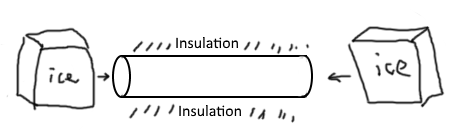
\includegraphics[width=0.7\textwidth]{heat_eq.PNG}} \end{center}
In order to figure out the temperature distribution $u(x,t)$, we need an equation that governs the change of temperature, which is called the \textbf{heat equation \index{heat equation}}. Usually, differential equation text books start with the Newton's cooling law to derive the one dimensional heat equation. However, we will approach it more heuristically by thinking of an example.
Let's say the entire rod was at the room temperature 20 degrees Celsius (=68 degrees Fahrenheit). If the rod is 2 meters long, the graph of the temperature distribution will be as follows:
\begin{center} \makebox[\textwidth]{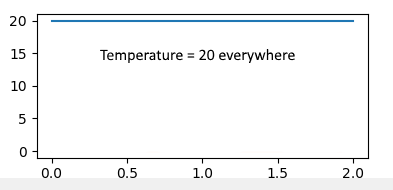
\includegraphics[width=0.7\textwidth]{heatgraph1.PNG}} \end{center}
Then, attach the ice at the end points so that the temperature at end points quickly drop to 0 degree Celsius. A brief moment later, we will have the following temperature distribution:
\begin{center} \makebox[\textwidth]{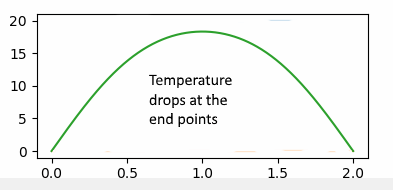
\includegraphics[width=0.7\textwidth]{heatgraph2.PNG}} \end{center}
Then as time goes by, the temperature will overall drop down to zero:
\begin{center} \makebox[\textwidth]{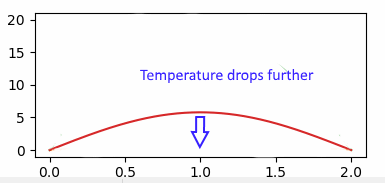
\includegraphics[width=0.7\textwidth]{heatgraph3.PNG}} \end{center}
What kind of behavior can we deduce from the above discussion? Well, we see that whether the temperature rises or falls at a point is related to the shape of the temperature graph near by. For example, at the center of the last picture above, the temperature is bent like an upside down U, and the temperature at the center decreases.
In mathematics, when a graph is bent like a U, we say the graph is concave up. So we know that the increase/decrease of the temperature at a point is related to concavity. Recall that concavity is measured by the second derivative. A way to remember the relationship between concave up/down and the sign of the second derivative is shown in the table below:
\begin{center} \makebox[\textwidth]{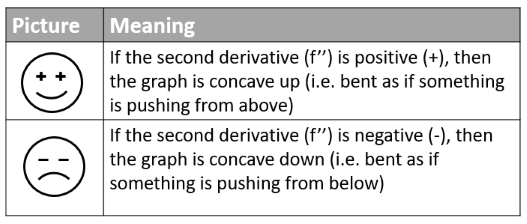
\includegraphics[scale=0.7]{concave_up_down.PNG}} \end{center}
The smiley face 'smiles' in a 'concave up' way and the frowning face 'frowns' in a 'concave down' way.
Not only that, you should convince yourself that the more concave the function is at a point, the faster the rate of change of the function will be. What is 'rate of change' in math? It is the derivative. But we have to be careful because there is two kinds of derivative at work. Since $u(x,t)$ is a function of $x$ and $t$, there is the derivative with respect to $x$ and a derivative with respect to $t$. 'Rate of change' is the change of temperature with respect to time, so it should be thought as the partial derivative
$$\frac{\partial u}{\partial t}(x,t).$$
On the other hand, 'concavity' is the shape of the temperature when drawn with the x-axis (which are the three temperature graphs we have seen before). So concavity should be measured by derivative of $x$ as:
$$\frac{\partial^2 u}{\partial x^2}(x,t)$$
Now, the previous discussion says that the two partial derivatives are related in the following way: If $\frac{\partial^2 u}{\partial x^2}(x,t)$ is positive, then the temperature graph is shaped like a U, and the temperature at the point will increase, i.e. $\frac{\partial u}{\partial t}(x,t)$ is positive. Same kind of statement can be said for the negative case. Not only that, since more concavity means faster rate of change, we can write:
$$\frac{\partial u}{\partial t} (x,t) \propto \frac{\partial^2 u}{\partial x^2}(x,t)$$
which is equivalent to saying:
$$\frac{\partial u}{\partial t}(x,t) = k \frac{\partial u}{\partial t}(x,t)$$
for some positive constant $k$. The above is what we call the \textit{heat equation}. Since this differential equation involves partial differentiation, it is an example of a \textit{partial differential equation}. It is one of the simplest partial differential equations, and it can be solved by hand in many easy cases.

Putting everything together, the heat equation along with the initial condition and boundary conditions, we have the full set of equations describing the behavior of the temperature distribution of a 1-dimensional rod:
$$\frac{\partial u}{\partial t}(x,t) = k \frac{\partial^2 u}{\partial x^2}(x,t)\; , \; \; 0<x<L, t>0$$
$$u(x,0)=u_0(x)  \; , \; \; 0<x<L$$
$$u(0,t)=u(L,t)=0 \; , \; \; t>0$$

There is another type of boundary condition that is also used often. That is the case when the end points are insulated. In that case we say that there is no change in the temperature across the end points, i.e. the derivative in the x direction is zero at the end points. This is written as:
$$\frac{\partial u}{\partial t}(x,t) = k \frac{\partial^2 u}{\partial x^2}(x,t)\; , \; \; 0<x<L, t>0$$
$$u(x,0)=u_0(x)  \; , \; \; 0<x<L$$
$$\frac{\partial u}{\partial x}(0,t)=\frac{\partial u}{\partial x}(L,t)=0 \; , \; \; t>0$$
As you can see, the last line has the boundary condition that describes insulated end points. Such boundary conditions are called \textit{Neumann boundary conditions}.

When instead of insulation, the end points are given some fixed value (such as zero as we have in the previous one) for all time, we call it \textit{Dirichlet boundary conditions}.


\subsection*{Solution of the heat equation}

Before we solve partial differential equations, I want to talk about constant functions. If a function is defined as $f(x)=1$, it means it's a function of $x$, but the value of the function is independent of $x$. It gives you the value of $1$ whatever $x$ value you put in. In a multivariable situation, say $f(x,t)$, you can have a function which is independent of $x$ but dependent in $t$ or vice-versa. 

For example, $f(x,t)=t+2$ would be a function of $x$ and $t$ whose value doesn't really depend on what you plug in for $x$. You can say that such a function is constant with respect to $x$. Any function of the form $f(x,t)=g(t)$ would be a function that is constant in $x$, because there is no $x$ involved in the definition of the function $f(x,t)$.

Now, suppose you were given a function $f(x,t)$. Initially, from the way it's written, you would assume that the function is dependent on $x$ and $t$. However, let's say you found that the function can be written as $f(x,t)=g(x)$ for some function $g(x)$. What does it mean? It means that the function is independent of $t$. Then, let's say you also found that $f(x,t)=h(t)$ for some function $h(t)$. This means that the function is independent of $x$ too. If a function $f(x,t)$ is independent of both $x$ and $t$, then the conclusion will be that the function's output doesn't depend on anything you plug in - whether you plug different values in $x$ or $t$ - and therefore, it must be a constant.

It's like playing with a toy which has two dials $x$ and $t$. If  $f(x,t)=g(x)$, then it means changing the dial $t$ doesn't change the outcome in any way. If $f(x,t)=h(t)$, then it means changing the dial $x$ doesn't change the outcome in any way. If both are true, then the toy's dials are meaningless decorations that don't do anything. (Think of activity walkers for babies that can't walk. Ones that look like cars would have handles that don't do anything.)
The reason for this discussion will be apparent later in the solution of the heat equation.

Now, let's actually solve one of these equations. Say we have:

\begin{ex}
$$\frac{\partial u}{\partial t}(x,t) = 3 \frac{\partial^2 u}{\partial x^2}(x,t)\; , \; \; 0<x<L, t>0$$
$$u(0,t)=u(2,t)=0 \; , \; \; t>0$$
$$u(x,0)=4  \; , \; \; 0<x<L$$
\end{ex}

The above means that the end points are set to 0 degrees Celsius and the initial temperature was 4 degrees everywhere. $k$ value is given as 3, and it controls how rapidly the heat spreads.

\textbf{Step 1} We solve this by using a method called \textbf{separation of variables\index{separation of variables}}. The idea is to \\
(A) only consider the heat equation and the boundary conditions at first (i.e. ignore the $u(x,0)=4$ for a moment.) \\
(B) assume that the solution takes the form of:
$$u(x,t)= f(x)\cdot g(t)$$
Which means that the function $u(x,t)$ is a product of a function of $x$ and a function of $t$. This is where the name 'separation of variables' come from. Let's compute the partial derivatives in order to plug into the heat equation:
$$\frac{\partial u}{\partial t}(x,t) = f(x)\cdot g'(t)$$
$$\frac{\partial^2 u}{\partial x^2}(x,t) = f''(x)\cdot g(t)$$
Then the heat equation becomes:
$$\frac{\partial u}{\partial t}(x,t) = 3 \frac{\partial^2 u}{\partial x^2}(x,t)  \; \rightarrow \; \; f(x)\cdot g'(t) = 3 f''(x)\cdot g(t) $$
Here is the \textit{IMPORTANT STEP}. You should divide both sides by $k f(x) g(t)$. (Many books, and some of my later sections use $X(x)$ and $T(t)$ instead of $f(x)$ and $g(t)$. In that case you would divide both sides by $kXT$.)
The result is:
$$\frac{f(x)\cdot g'(t)}{3f(x)g(t)} = \frac{3 f''(x)\cdot g(t)}{3f(x)g(t)}  \; \rightarrow \; \; \frac{g'(t)}{3g(t)} = \frac{ f''(x)}{f(x)} $$
Now comes an interesting argument. First, you see that the above equation involves two independent variables $x$ and $t$. So let's assign it as a function $H(x,t)$:
$$H(x,t):=\frac{g'(t)}{3g(t)} = \frac{ f''(x)}{f(x)} $$
But then, looking at $H(x,t)=\frac{g'(t)}{3g(t)}$, we see that $H(x,t)$ does not depend on $x$. On the other hand, looking at $H(x,t) = \frac{ f''(x)}{f(x)} $, we see that $H(x,t)$ does not depend on $t$. What does that say about $H(x,t)$? It means that it's a constant function, as we have discussed in the beginning of this section. For a reason that will be apparent later, we will call that constant $-\lambda$. So we have the following equality:
$-\lambda=\frac{g'(t)}{3g(t)} = \frac{ f''(x)}{f(x)} $
This leads to two equations:
$-\lambda=\frac{g'(t)}{3g(t)} $
and
$-\lambda= \frac{ f''(x)}{f(x)} $
This last equation turns into
$$f''(x) + \lambda f(x) =0$$
This looks familiar. When we solved the eigenfunction-eigenvalue problem for Endpoint Value Problem, we had $x''(t) + \lambda x(t)=0$. The above question is same, if we take $f$ to be $x$ and $x$ to be $t$. In fact, the whole point of eigenfunction-eigenvalue problem was that it was needed in order to solve PDEs. We will come back to this in a moment.

\textbf{Step 2} Next we consider the boundary conditions. Recall that $u(x,t)=f(x)g(t)$. The boundary condition $u(0,t)=u(2,t)=0$ then turns into $f(0)g(t)=f(2)g(t)=0$. We see from $f(0)g(t)=0$ that either $f(0)=0$ or $g(t)=0$. However, $g(t)=0$ leads to $u(x,t)=f(x)g(t)=f(x)\cdot 0=0$. So that part is not that interesting. (It is certainly a solution satisfying the heat equation and the boundary conditions, albeit something anyone can easily see without having to do all this work. This solution is called the \textbf{trivial solution\index{trivial solution}}.) Therefore, in order to have useful solutions, we must have $f(0)=0$. For the same reason, we use $f(2)g(t)=0$ to get $f(2)=0$.


\textbf{Step 3} Now take the previous equation $f''(x) + \lambda f(x) =0$ along with the boundary conditions $f(0)=0$ and $f(2)=0$. This is indeed the eigenfunction-eigenvalue problem with end point conditions that we have seen before. We know that when the end points are set to zero, the only kind of non-trivial solutions are $f(x)=\sin \frac{n\pi}{2} x$ with the eigenvalue $\lambda = \frac{n^2 \pi^2}{4}$ for $n=1,2,3, \cdots $.

For $g(t)$, we had $-\lambda=\frac{g'(t)}{3g(t)} $. Plugging in $\lambda = \frac{n^2 \pi^2}{4}$ and multiplying 3 both sides, we have:
$$-3\frac{n^2 \pi^2}{4}=\frac{g'(t)}{g(t)} $$
Integrating both sides, we have:
$$-3\frac{n^2 \pi^2}{4} t + \tilde{C} = \ln g(t) $$
Then exponentiating, we have:
$$g(t) = C e^{-3\frac{n^2 \pi^2}{4} t}$$
Since we have found out what $f(x)$ and $g(t)$ could be, we know what $u(x,t)$ is:
$$u(x,t) = C f(x) g(t) = C \sin \left(\frac{n\pi}{2} x \right) e^{-3\frac{n^2 \pi^2}{4} t}$$
What you should notice in the above solution is that this is not just one solution but infinitely many solutions for $n=1,2,3, \cdots $.

\textbf{Step 4} Think about how in homogeneous differential equations when we could take linear combinations of solutions to form a solution. The same is true for our case too. (You can check this by assuming that $u_1(x,t)$ and $u_2(x,t)$ both satisfy the heat equation and the boundary conditions and then trying to plug in $u(x,t) = c_1 u_1(x,t) + c_2 u_2(x,t)$. ) The only difference in this case would be that since we have infinitely many solutions, adding them all gives us the infinite series, written as:
$$u(x,t) = \sum_{n=1}^{\infty} c_n \sin \left(\frac{n\pi}{2} x \right) e^{-\frac{3n^2 \pi^2}{4} t}$$
You can think of the above as the general solution for our heat equation. The only thing we haven't included in our consideration is the initial condition $u(x,0)=4$. We will do so in the next section.

\textbf{Step 5} We now have:
$$u(x,t) = \sum_{n=1}^{\infty} c_n \sin \left(\frac{n\pi}{2} x \right) e^{-\frac{3n^2 \pi^2}{4} t}$$
To match this with $u(x,0)=4$, we will plug in $t=0$ into the above equation. Since $e^0 =0$, the entire exponential factor disappears when $t=0$ is plugged in. Setting it equal to $4$:
$$4 = \sum_{n=1}^{\infty} c_n \sin \left(\frac{n\pi}{2} x \right) $$
This looks familiar. This is the Fourier Series, or Fourier sine series to be exact. Since we need $u(x,0)=4$ to hold when $0<x<2$, we need to find the Fourier sine series of $4$ in order to make sense out of the above equation. We compute:
$$b_n = \frac{2}{2} \int_{0}^{2} 4\cdot \sin \left(\frac{n\pi}{2} x \right)dx$$
$$= 4\cdot \left(-\frac{2}{n\pi} \cos \left(\frac{n\pi}{2} x \right) \right) \Bigg\vert_0^2$$
$$= -\frac{8}{n\pi} \left( (-1)^n -1 \right)$$
$$= \frac{8}{n\pi} \left( 1-(-1)^n  \right)$$

\textbf{Step 6} Okay, so we now know that:
$$4 = \sum_{n=1}^{\infty} \frac{8}{n\pi} \left( 1-(-1)^n  \right)\sin \left(\frac{n\pi}{2} x \right) $$
from the Fourier sine series. If you look closely, you see that in place of $c_n$ we had before, we now have $\frac{8}{n\pi} \left( 1-(-1)^n  \right)$. Thus we found that:
$$c_n=\frac{8}{n\pi} \left( 1-(-1)^n  \right)$$
Plugging this back into the $u(x,t)$ formula in the beginning of this section, we get the final answer:
$$u(x,t) = \sum_{n=1}^{\infty} c_n \sin \left(\frac{n\pi}{2} x \right) e^{-\frac{3n^2 \pi^2}{4} t}$$

\subsection*{Plot of the heat equation}
Using a computer one can plot the graph of
$$u(x,t) = \sum_{n=1}^{\infty} c_n \sin \left(\frac{n\pi}{2} x \right) e^{-3\frac{n^2 \pi^2}{4} t}$$
For example, I used a programming language called python, with the pylab package, to draw the graph of $u(x,t)$ for various values of $t$ :
\begin{center} \makebox[\textwidth]{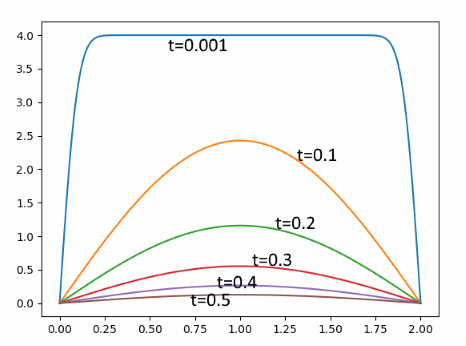
\includegraphics[width=0.7\textwidth]{heat_eq_plot.PNG}} \end{center}
As you can see, the temperature will eventually become zero everywhere.

For those who are curious to know, here is the python (with pylab) code used to generate the above graph. (People who know matlab will find that it is very similar to matlab)

\begin{lstlisting}
from pylab import *
x=linspace(0,2,1001)
t=linspace(0,1,1001)
fs=zeros((1001,1001))
for n in range(1,1000,2):
	fs[n,:]=16*sin(n*pi*x/2)/(n*pi)
T=zeros((1001,1001))
for n in range(0,1001):
	T[n,:]=exp(-3*n*n*pi*pi*t/4)
u=dot(transpose(T),fs)
plot(x,u[1,:])
plot(x,u[100,:])
plot(x,u[200,:])
plot(x,u[300,:])
plot(x,u[400,:])
plot(x,u[500,:])
\end{lstlisting}


\subsection*{Heat Equation with Neumann boundary conditions }
\begin{ex} Solve the heat equation with Neumann boundary conditions:
$$u_t(x,t) = 7 u_{xx}(x,t)\; , \; \; 0<x<L, t>0$$
$$u(x,0)=-x+6  \; , \; \; 0<x<L$$
$$u_x(0,t)=u_x(8,t)=0 \; , \; \; t>0$$
(Note: We are using the notation $u_t$ for $\frac{\partial u}{\partial t}$, and so on.)
\end{ex}
Solution)
Separation of variables:
$$u(x,t)=X(x)T(t)$$
$$u_t(x,t) = X(x) T'(t)$$
$$u_{xx}(x,t) = X''(x) T(t)$$
$$u_t(x,t) = 7 u_{xx}(x,t)  \; \rightarrow \; X(x) T'(t) = 7 X''(x) T(t) $$
Divide both sides by $7X(x)T(t)$.
$$\frac{X(x) T'(t)}{7X(x)T(t)} = \frac{7 X''(x) T(t)}{7X(x)T(t)}  \; \rightarrow \; \; \frac{T'(t)}{7T(t)} = \frac{X''(x)}{X(x)} $$
Then since the left side is independent of $x$ and the right side is independent of $t$, we know that the only way they could be equal is if they are both equal to a constant. We will call that constant $-\lambda$, so that:
$$-\lambda=\frac{T'(t)}{7T(t)} = \frac{X''(x)}{X(x)} $$
From the boundary conditions:
$$u_x(0,t)=u_x(8,t)=0  \; \rightarrow \; X'(0)T(t)=X'(8)T(t)=0$$
Since $T(t)=0$ would give a trivial solution, we must have $T(t)\neq0$ and the above forces $X'(0)=X'(8)=0$.
Then we have the following eigenfunction-eigenvalue problem:
$$-\lambda = \frac{X''(x)}{X(x)}  \; \rightarrow \; X''(x) + \lambda X(x) =0$$
with the end point condition $X'(0)=X'(8)=0$. We have solved such problems before. When the end point conditions say the derivative is zero, then we have the cosine functions as the eigenfunctions. We have
$$X(x) = \cos \left( \frac{n \pi}{8} x \right)   \; , \; \; \lambda = \frac{n^2 \pi^2}{64} $$
for $n=0,1,2,3, \cdots $.
Also, since $-\lambda=\frac{T'(t)}{7T(t)}$, solving it gives us: $T(t) = C e^{-7\lambda t}$. Using the eigenvalues we found, we obtain:
$$T(t) =  C e^{-\frac{7n^2 \pi^2}{64} t}$$
We have the solutions:
$$u(x,t) = C \cos \left( \frac{n \pi}{8} x \right) e^{-\frac{7n^2 \pi^2}{64} t}$$
for $n=0,1,2,3, \cdots $.
We move on to take the linear combination of these solutions  make this into a series:
$$u(x,t) = \sum_{n=0}^{\infty} c_n \cos \left( \frac{n \pi}{8} x \right) e^{-\frac{7n^2 \pi^2}{64} t}$$
Now, when $n=0$, we have $\cos \left( \frac{n \pi}{8} x \right) e^{-\frac{7n^2 \pi^2}{64} t} =\cos 0 \cdot e^0 = 1$. Therefore we just have $c_0$ by itself if $n=0$. So we have:
$$u(x,t) = c_0 + \sum_{n=1}^{\infty} c_n \cos \left( \frac{n \pi}{8} x \right) e^{-\frac{7n^2 \pi^2}{64} t}$$

Let's apply the initial condition
$$u(x,0)=-x+6  \; , \; \; 0<x<L$$
Putting $t=0$ makes $e^{-\frac{7n^2 \pi^2}{64} t}=1$ and thus:
$$-x+6 = c_0 + \sum_{n=1}^{\infty} c_n \cos \left( \frac{n \pi}{8} x \right) $$
Thus this suggests taking the Fourier cosine series of $-x+6$. So we compute:
$$a_0 = \frac{2}{8} \int_0^8 (-x+6) dx = \frac{1}{4} \left( -\frac{1}{2}x^2 + 6x \right) \Bigg\vert_0^8 = 4$$
and
$$a_n = \frac{2}{8} \int_0^8 (-x+6) \cos \left( \frac{n \pi}{8} x \right) dx $$
$$ = \frac{2}{8} \left[ (-x+6)\cdot \frac{8}{n \pi} \sin \left( \frac{n \pi}{8} x \right) - \frac{64}{n^2 \pi^2} \cos \left( \frac{n \pi}{8} x \right) \right] \Bigg\vert_0^8$$
$$ =  - \frac{16}{n^2 \pi^2} \left( (-1)^n -1 \right) =   \frac{16}{n^2 \pi^2} \left( 1-  (-1)^n \right) $$
Thus the Fourier Cosine law tells us:
$$-x+6 = \frac{4}{2} + \sum_{n=1}^{\infty} \frac{16}{n^2 \pi^2} \left( 1-  (-1)^n \right)  \cos \left( \frac{n \pi}{8} x \right) $$
Comparing, we see that $c_0 =\frac{4}{2} =2$ while $c_n = \frac{16}{n^2 \pi^2} \left( 1-  (-1)^n \right)$. Thus the general solution is:
$$u(x,t) = 2 + \sum_{n=1}^{\infty} \frac{16}{n^2 \pi^2} \left( 1-  (-1)^n \right)  \cos \left( \frac{n \pi}{8} x \right) e^{-\frac{7n^2 \pi^2}{64} t} $$

\subsection*{Heat equation solution that do not require Fourier Series}
Think about the following example:
\begin{ex}
$$\frac{\partial u}{\partial t}(x,t) = 0.2 \frac{\partial^2 u}{\partial x^2}(x,t)\; , \; \; 0<x<L, t>0$$
$$u(0,t)=u(3,t)=0 \; , \; \; t>0$$
$$u(x,0)=\cos(6\pi x) - \cos(2\pi x) + 7  \; , \; \; 0<x<L$$
\end{ex}

Solution)
Separation of variables:
$$u(x,t)=X(x)T(t)$$
$$u_t(x,t) = X(x) T'(t)$$
$$u_{xx}(x,t) = X''(x) T(t)$$
$$u_t(x,t) = 0.2 u_{xx}(x,t)  \; \rightarrow \; X(x) T'(t) = 0.2 X''(x) T(t) $$
Divide both sides by $7X(x)T(t)$.
$$\frac{X(x) T'(t)}{0.2X(x)T(t)} = \frac{0.2 X''(x) T(t)}{0.2X(x)T(t)}  \; \rightarrow \; \; \frac{T'(t)}{0.2T(t)} = \frac{X''(x)}{X(x)} $$
Then since the left side is independent of $x$ and the right side is independent of $t$, we know that the only way they could be equal is if they are both equal to a constant. We will call that constant $-\lambda$, so that:
$$-\lambda=\frac{T'(t)}{0.2T(t)} = \frac{X''(x)}{X(x)} $$
From the boundary conditions:
$$u_x(0,t)=u_x(3,t)=0  \; \rightarrow \; X'(0)T(t)=X'(3)T(t)=0$$
Since $T(t)=0$ would give a trivial solution, we must have $T(t)\neq0$ and the above forces $X'(0)=X'(3)=0$.
Then we have the following eigenfunction-eigenvalue problem:
$$-\lambda = \frac{X''(x)}{X(x)}  \; \rightarrow \; X''(x) + \lambda X(x) =0$$
with the end point condition $X'(0)=X'(3)=0$. We have solved such problems before. When the end point conditions say the derivative is zero, then we have the cosine functions as the eigenfunctions. We have
$$X(x) = \cos \left( \frac{n \pi}{3} x \right)   \; , \; \; \lambda = \frac{n^2 \pi^2}{9} $$
for $n=0,1,2,3, \cdots $.
Also, since $-\lambda=\frac{T'(t)}{0.2T(t)}$, solving it gives us: $T(t) = C e^{-0.2\lambda t}$. Using the eigenvalues we found, we obtain:
$$T(t) =  C e^{-\frac{0.2n^2 \pi^2}{9} t}$$
We have the solutions:
$$u(x,t) = C \cos \left( \frac{n \pi}{3} x \right) e^{-\frac{0.2 n^2 \pi^2}{9} t}$$
for $n=0,1,2,3, \cdots $.
Just as before we take the linear combination:
$$u(x,t) = c_0 + \sum_{n=1}^{\infty} c_n \cos \left( \frac{n \pi}{3} x \right) e^{-\frac{0.2 n^2 \pi^2}{9} t}$$

However when we look at the initial condition $u(x,0)=\cos(6\pi x) - \cos(2\pi x) + 7 $ and set it equal with $t=0$:
$$\cos(6\pi x) - \cos(2\pi x) + 7  =  c_0 + \sum_{n=1}^{\infty} c_n \cos \left( \frac{n \pi}{3} x \right) $$
We see that already we can make $c_0=7$ and then the two other terms $\cos(6\pi x) - \cos(2\pi x)$ are already sums of cosines. Let's try to find out when $\frac{n \pi}{3} =6 \pi$ or when $\frac{n \pi}{3} =2 \pi$. We have $n=18$ and $ n=6$. In other words, if we take $c_0=7$, $c_6=-1$, $c_{18}=1$ and set all other $c_n$ as zero then the above equality holds. This is a case where we did not have to find the Fourier cosine series in order to find the coefficients, because the initial condition is already given to us as a Fourier cosine series.

Plugging in $c_0=7$, $c_6=-1$, $c_{18}=1$ and set all other $c_n$ as zero, we have the answer:
$$u(x,t) = 7 - \cos \left( 2\pi x \right) e^{-0.8 \pi^2 t}+\cos \left( 6\pi x \right) e^{-7.2\pi^2 t}$$

\section{Wave Equation}

\subsection*{Introduction to the wave equation}

Here is another example of a partial differential equation, which is called the wave equation. Picture a string tied at both ends (e.g. a guitar). When the string is plucked, the string vibrates rapidly to make a sound (which explains the name 'wave equation'). If we view the string motion, we see that the tension force acts against the bending of the string to bring it back to the straightened position, like in the picture shown below:
\begin{center} \makebox[\textwidth]{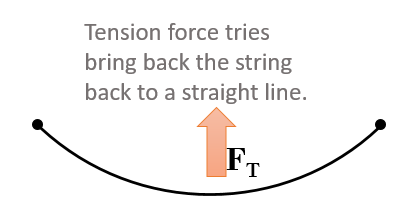
\includegraphics[width=0.7\textwidth]{string.PNG}} \end{center}
What does this mean? It means that the force is propotional to the bending, i.e. concavity:
$$ F \propto \frac{\partial^2 u}{\partial x^2}(x,t)$$
Here, $u(x,t)$ has the meaning of 'vertical displacement of the string at position $x$ at time $t$ '.
Since $F=ma$, we know that above statement means acceleration is proportional to concavity too:
$$ a \propto \frac{\partial^2 u}{\partial x^2}(x,t)$$
But then, acceleration is the second derivative in time, so we write:
$$ \frac{\partial^2 u}{\partial t^2}(x,t) \propto \frac{\partial^2 u}{\partial x^2}(x,t)$$
When we write this as an equation, we put the proportionality constant as $c^2$ to write:
$$ \frac{\partial^2 u}{\partial t^2}(x,t) = c^2 \frac{\partial^2 u}{\partial x^2}(x,t)$$
The above is a partial differential equation called the \textbf{wave equation \index{wave equation}}. The reason for using $c^2$ for the proportionality constant is because the solution of the equation becomes easier to write if we put it that way. (It also stresses the fact that $c^2$ is positive.)

Since it is a second order differential equation in time, we need to give two initial conditions:
$$u(x,0)=f(x)$$
and
$$\frac{\partial u}{\partial t}(x,0) = g(x)$$
The first gives the initial configuration of the string and the second gives the initial velocity of the string at each point $x$.

Also, the fixed end points of the string means that the vertical displacement is always zero at the end points. So we have:
$$u(0,t)=u(L,t)=0$$
where $L$ is the length of the string.

You can also have Neumann boundary conditions at the end points. Such conditions describe wind pipe instruments like flute or pipe organ. For wind instruments, $u(x,t)$ has the meaning of pressure (compared to the atmospheric pressure) at point $x$ at time $t$. If the wind instrument has open ends, then the pressure is zero (i.e. same as the atmospheric pressure) at the end points, so we have Dirichlet boundary conditions (set to zero). However, if one end is closed (as instruments like flute is, where the end close to the mouth piece is closed) then the derivative of $u(x,t)$ should be set to zero at that end point, giving us the Neumann boundary condition at that end.

To summarize, a vibrating string or a wind instrument with both ends open follows the partial differential equation and boundary conditions:
$$ \frac{\partial^2 u}{\partial t^2}(x,t) \propto \frac{\partial^2 u}{\partial x^2}(x,t) \; , \; \; 0<x<L, t>0$$
$$u(x,0)=f(x)  \; , \; \; \frac{\partial u}{\partial t}(x,0) = g(x)  \; , \; \; 0<x<L$$
$$u(0,t)=u(L,t)=0 \; , \; \; t>0$$


\subsection*{Solving Wave Equation using Fourier Series}

Suppose a string 4 in. long is tied at both ends. We pulle the string at the middle to make the following shape:

\begin{center} \makebox[\textwidth]{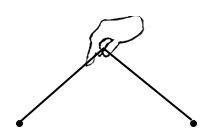
\includegraphics[scale=1.1]{pull_string.PNG}} \end{center}

Then we \textit{release} this string, meaning that the initial velocity of every part of the string will be zero. This can be written as $ y_t (x,0) = 0 $ for all $x$ in the interval $[0,4]$. We still have to provide a value for $c^2$ as explained in the previous section. Let's assume that we are given the value $c^2=9$. 

\begin{ex}
	Solve the wave equation using Fourier Series:
	$$ y_{tt} = 9 y_{xx} \; \; \; \;,  \; (0<x<4, \; t>0) $$
	$$ y(0,t) = y(4,t)=0, \; \; \; \;,  \; ( t>0) $$
	$$ y(x,0) = 4 - |2-x| \; \; \; \;,  \; (0<x<4) $$
	$$ y_t (x,0) = 0 \; \; \; \;,  \; (0<x<4) $$
	\end{ex}

Solution) 
We use the separation of variables method again. If you do not understand this method, please review how the heat equation was solved by separation of variables. 

\textbf{step 1.} We will find set of solutions that satisfy the wave equation and the boundary conditions.

Put
$$y(x,t) = X(x) T(t) $$
Plugging this into the wave equation, we get
$$ X(x) T''(t) = 9 X''(x) T(t) $$
Dividing both sides by $ 9 X(x) T(t) $ gives us
$$\frac{T''(t)}{9T(t)}= \frac{X''(x)}{X(x)}$$
Noticing that the left side doesn't change when $x$ changes and then that the right side doesn't change when $t$ changes, we can conclude that the above has to be a constant number. Call that constant number $-\lambda$ so that we have
$$\frac{T''(t)}{9T(t)}= \frac{X''(x)}{X(x)}=-\lambda$$
The equation $\frac{X''(x)}{X(x)}=-\lambda$ gives us 
$X''(x) + \lambda X(x) =0 $. Now, observe that the boundary conditions $ y(0,t) = y(4,t)=0$ in separation of variables is $X(0)T(t)=X(4)T(t)=0$. Since $T(t)=0$ leads to trivial solution, we are forced to say $X(0)=X(4)=0$. Thus we have the eigenvalue-eigenfunction problem:
$$ X''(x) + \lambda X(x) =0 \; \; \; , \; X(0)=X(4)=0.$$
The solution of this problem is (see the chapter Endpoint Value problems for details of how eigenfunctions and eigenvalues are found)
$$X(x)= C \sin\frac{n\pi x}{4} \;, \; n=1,2,3,4,\cdots$$
with
$$\lambda = \frac{n^2 \pi^2}{16} \;, \; n=1,2,3,4,\cdots$$

Then $\frac{T''(t)}{9T(t)}=-\lambda$ can now be written as (after multiplying $9T(t)$,
$$T''(t) = -\frac{9n^2 \pi^2}{16} T(t).$$
After moving everything to the left as $T''(t) + \frac{9n^2 \pi^2}{16} T(t)=0$, we can write the characteristic equation as
$$r^2 + \frac{9n^2 \pi^2}{16}=0$$
$$r =\pm \frac{3n\pi}{4} i$$
$$T(t) = C_1 \cos \frac{3n\pi}{4} t + C_2 \sin \frac{3n\pi}{4} t $$

Now, $y(x,t) = X(x) T(t) $ becomes
$$ y(x,t) =  C \sin\frac{n\pi x}{4} \left( C_1 \cos \frac{3n\pi}{4} t + C_2 \sin \frac{3n\pi}{4} t \right) =  C\cdot C_1 \sin\frac{n\pi x}{4} \cos \frac{3n\pi}{4} t + C\cdot C_2 \sin\frac{n\pi x}{4} \sin \frac{3n\pi}{4} t $$

Since $C\cdot C_1$ and $C\cdot C_2$ are arbitrary constants, we can reassign the name of them as $A_n$ and $B_n$ respectively. The reason for the subscript $n$ is because the above is actually an infinite set of solutions for $n=1,2,3,4,\cdots$. If we can take linear combinations of all of them, then we end up with the following series:

$$ y(x,t) = \sum_{n=1}^{\infty} A_n \sin\frac{n\pi x}{4} \cos \frac{3n\pi}{4} t + \sum_{n=1}^{\infty} B_n \sin\frac{n\pi x}{4} \sin \frac{3n\pi}{4} t $$

The linear combination satisfies the wave equation $ y_{tt} = 9 y_{xx}$ because it is linear. You should also check that it satisfies the boundary condition $ y(0,t) = y(4,t)=0, \; \; \; \;,  \; ( t>0) $.

\textbf{step 2.} We now put the initial value problem into consideration. First we consider $ y(x,0) = 4 - |2-x| \;,  \; (0<x<4) $. Setting $t=0$ in the solution obtained in step 1, we have:
$$ \sum_{n=1}^{\infty} A_n \sin\frac{n\pi x}{4} \left( \cos \frac{3n\pi}{4} \cdot 0 \right) + \sum_{n=1}^{\infty} B_n \sin\frac{n\pi x}{4} \left( \sin \frac{3n\pi}{4} \cdot 0 \right) = 4 - |2-x| $$
The second summation becomes zero because $\sin 0 =0$. So using $\cos 0 =1$ we get:
$$ \sum_{n=1}^{\infty} A_n \sin\frac{n\pi x}{4} = 4 - |2-x| $$

This means that in order to find out the values of $A_n$'s, we need to find the Fourier sine expansion of the right side. We use the Fourier sine formula with $L=4$ to get

$$b_n = \frac{2}{4} \int_{0}^{4} (4 - |2-x|) \sin \frac{n\pi}{4} x dx$$
$$ \; \; \; = \frac{1}{2} \left( \int_{0}^{2} (4 - |2-x|) \sin \frac{n\pi}{4} x dx \right) + \frac{1}{2} \left( \int_{2}^{4} (4 - |2-x|) \sin \frac{n\pi}{4} x dx \right) $$
$$ \; \; \; = \frac{1}{2} \left( \int_{0}^{2} (4 - (2-x)) \sin \frac{n\pi}{4} x dx \right) + \frac{1}{2} \left( \int_{2}^{4} (4 - (x-2)) \sin \frac{n\pi}{4} x dx \right) $$
$$ \; \; \; = \frac{1}{2} \left( \int_{0}^{2} (2+x) \sin \frac{n\pi}{4} x dx \right) + \frac{1}{2} \left( \int_{2}^{4} (6 - x) \sin \frac{n\pi}{4} x dx \right) $$
Perform the integration by parts (or tabular integration) for each integral to get:
$$ \; \; \; = \frac{1}{2} \left. \left( -\frac{4}{n\pi} (2+x) \cos \frac{n\pi}{4} x + \frac{16}{n^2\pi^2} \sin \frac{n\pi}{4} x \right) \right\vert_0^2 + \frac{1}{2} \left. \left( -\frac{4}{n\pi} (6 - x) \cos \frac{n\pi}{4} x  - \frac{16}{n^2\pi^2} \sin \frac{n\pi}{4} x \right)\right\vert_2^4 $$
$$ \; \; \; = \frac{1}{2} \left( -\frac{16}{n\pi} \cos \frac{n\pi}{2}  + \frac{16}{n^2\pi^2} \sin \frac{n\pi}{2} - \left(-\frac{8}{n\pi}  \right) \right) + \frac{1}{2} \left( -\frac{8}{n\pi} \cos n\pi  - \left( -\frac{16}{n\pi} \cos \frac{n\pi}{2}  - \frac{16}{n^2\pi^2} \sin \frac{n\pi}{2} \right) \right)  $$
$$ \; \; \; = -\frac{8}{n\pi} \cos \frac{n\pi}{2}  + \frac{8}{n^2\pi^2} \sin \frac{n\pi}{2} + \frac{4}{n\pi}     -\frac{4}{n\pi} \cos n\pi  +\frac{8}{n\pi} \cos \frac{n\pi}{2}  + \frac{8}{n^2\pi^2} \sin \frac{n\pi}{2}  $$
$$ \; \; \; =  \frac{16}{n^2\pi^2} \sin \frac{n\pi}{2} + \frac{4}{n\pi}     -\frac{4}{n\pi} \cos n\pi  $$


Now, depending on whether $n$ is even (which can be expressed as $n=2m$ for some integer $m$) or odd (which can be expressed as $n=2m+1$ for some integer $m$), the above can be further simplified using $\sin \frac{2m\pi}{2} = \sin m\pi =0 $ and $\sin \frac{(2m+1)\pi}{2} = (-1)^m$. If $n=2m$, we get:
$$ \frac{16}{n^2\pi^2} \sin \frac{n\pi}{2} + \frac{4}{n\pi}     -\frac{4}{n\pi} \cos n\pi = \frac{16}{n^2\pi^2} \sin \frac{2m\pi}{2} + \frac{4}{n\pi}     -\frac{4}{n\pi} \cos 2m\pi = 0 +\frac{4}{n\pi}  - \frac{4}{n\pi} =0$$
If $n=2m+1$, we get:

$$ \frac{16}{n^2\pi^2} \sin \frac{n\pi}{2} + \frac{4}{n\pi}     -\frac{4}{n\pi} \cos n\pi =\frac{16}{n^2\pi^2} \sin \frac{(2m+1)\pi}{2} + \frac{4}{n\pi}     -\frac{4}{n\pi} (-1) = \frac{16}{n^2\pi^2} (-1)^m + \frac{8}{n\pi}  $$
If we replace all the remaining $n$ by $2m+1$ we have
$$\frac{16}{(2m+1)^2\pi^2} (-1)^m + \frac{8}{(2m+1)\pi} $$

The Fourier sine series we obtain is therefore
$$ 4 - |2-x| = \sum_{n=1}^{\infty}  b_n \sin \frac{n\pi}{4} x = \sum_{m=0}^{\infty}  \left( \frac{16}{(2m+1)^2\pi^2} (-1)^m + \frac{8}{(2m+1)\pi}  \right) \sin \frac{(2m+1)\pi}{4} x$$

Note that the summation starts from $m=0$ because then $n=2m+1=2\cdot0+1=1$. Now this means for $A_n$'s : 

$$ \sum_{n=1}^{\infty} A_n \sin\frac{n\pi x}{4} = \sum_{m=0}^{\infty}  \left( \frac{16}{(2m+1)^2\pi^2} (-1)^m + \frac{8}{(2m+1)\pi}  \right) \sin \frac{(2m+1)\pi}{4} x$$
This yields that if $n$ is even, $A_n=0$. For $n$ odd, we have:
$$ A_{2m+1} = \frac{16}{(2m+1)^2\pi^2} (-1)^m + \frac{8}{(2m+1)\pi} $$

We still have the other initial condition $ y_t (x,0) = 0$. If we differentiate (by $t$)
$$ y(x,t) = \sum_{n=1}^{\infty} A_n \sin\frac{n\pi x}{4} \cos \frac{3n\pi}{4} t + \sum_{n=1}^{\infty} B_n \sin\frac{n\pi x}{4} \sin \frac{3n\pi}{4} t $$
to get
$$ y(x,t) = \sum_{n=1}^{\infty} -A_n \frac{3n\pi}{4} \sin\frac{n\pi x}{4} \sin \frac{3n\pi}{4} t + \sum_{n=1}^{\infty} B_n \frac{3n\pi}{4}  \sin\frac{n\pi x}{4} \cos \frac{3n\pi}{4} t .$$

Then 
$$y(x,0) = \sum_{n=1}^{\infty} B_n \frac{3n\pi}{4}  \sin\frac{n\pi x}{4} $$
Setting this equal to $ y_t (x,0) = 0$ we have
$$\sum_{n=1}^{\infty} B_n \frac{3n\pi}{4}  \sin\frac{n\pi x}{4} =0$$
Which suggests that we must find the Fourier sine series of the right side. However, the function $0$ of the right side has the Fourier sine series $0$. Hence
$$B_n \frac{3n\pi}{4} =0 $$
and we end up with $B_n=0$ for all $n$. So the second summation in $y(x,t)$ completely disappears.

We finally arrive at the solution
\begin{align*}
y(x,t) &= \sum_{n=1}^{\infty} A_n \sin\frac{n\pi x}{4} \cos \frac{3n\pi t}{4} \\
&= \sum_{m=0}^{\infty}  \left( \frac{16}{(2m+1)^2\pi^2} (-1)^m + \frac{8}{(2m+1)\pi}  \right) \sin \frac{(2m+1)\pi x }{4}  \cos \frac{3(2m+1)\pi t}{4}\\
\end{align*}



\chapter{Laplace Transform Method}

\section{Laplace Transform and Its Inverse}

\subsection*{Introduction to Laplace Transforms}

A transform is an operation where it takes in a function and returns a function of a different variable. Among such transforms, one transform called Laplace transform is used for solving differential equations. It is defined as:
$$ \mathscr{L} \left\{ f(t) \right\}= \int_0^{\infty}  e^{-st} f(t) dt $$
where $s$ is assumed to be bigger than some positive number (just a technicality assumed in order to make the integral converge.)
The best way to understand what the above formula is doing is to try out an example:
$$ \mathscr{L} \left\{t^2 \right\}= \int_0^{\infty} e^{-st} t^2 dt$$
We use integration by parts (or tabular integration) to do the integration. The result is:

$$ = \left(-\frac{t^2}{s} e^{-st} -\frac{2t}{s^2} e^{-st} - \frac{2}{s^3} e^{-st} \right) \Bigg\vert_0^{\infty} $$
When $t=\infty$ is plugged into $e^{-st}$, since $s$ is positive, we get $e^{-\infty}$ which is equal to zero. Thus we only get zero for all the terms when $t=\infty$ is plugged in. For the case when $t=0$ is plugged in, anything that has $t$ or $t^2$ multiplied will be zero. Thus the only non-zero result you will get is when $t=0$ is plugged into $- \frac{2}{s^3} e^{-st} $, and since it is subtracted, the result is :
$$\frac{2}{s^3}$$

So the result is that
$$ \mathscr{L} \left\{t^2\right\}= \frac{2}{s^3}$$
\textit{As you can see, a function of} $t$ \textit{was plugged in and the result is a function of} $s$.

You can calculate similarly to get the following results:
$$ \mathscr{L} \left\{t\right\}= \frac{1}{s^2}$$
$$ \mathscr{L} \left\{1\right\}= \frac{1}{s}$$

In general, you have:
$$ \mathscr{L} \left\{t^n\right\}= \frac{n!}{s^{n+1}}$$
where $n!$ means $n!=1\cdot 2 \cdot 3 \cdots n$

There are results of the Laplace transform of other functions. These are provided to you as a table \index{Table of Laplace Transforms} shown below:

\begin{center} \makebox[\textwidth]{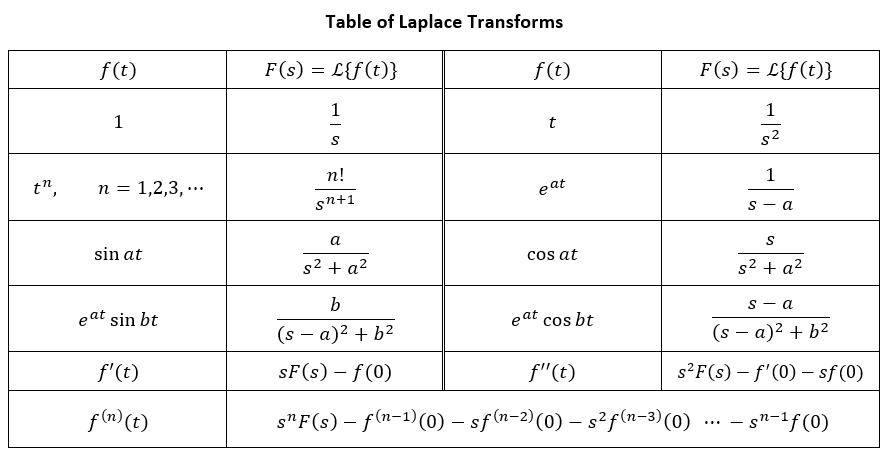
\includegraphics[width=\textwidth]{laplace_table.PNG}} \end{center}


\subsection*{Laplace transform of derivatives and differential equations }

Suppose $F(s)$ is the Laplace transform of $f(t)$. In other words, we have $ \mathscr{L} \left\{f(t) \right\} = F(s)$. Then the derivative of $f(t)$ transforms according to the following formula:
$$ \mathscr{L} \left\{f'(t) \right\} = sF(s)-f(0)$$
\textit{Proof} The proof is an easy application of the integration by parts.
$$ \mathscr{L} \left\{f'(t) \right\} = \int_0^{\infty} e^{-st} f'(t) dt $$
Take $dv=f'(t)dt$ so that $v=f(t)$. Also $u= e^{-st}$ so that $du = -s e^{-st} dt$. Then the integration by parts formula $\int u dv = uv - \int v du $ becomes:
$$\int_0^{\infty} e^{-st} f'(t) dt = e^{-st} f(t) \Bigg\vert_0^{\infty} - \int_0^{\infty} -s e^{-st} f(t) dt. $$
Now, $e^{-st} f(t) \Bigg\vert_0^{\infty} = e^{-\infty}f(\infty) - e^0 f(0) =0-f(0)$. (Small technicality:  we are assuming that $f(t)$ doesn't increase too fast so that the limit to infinity is zero.) Also, since the second integral is the integration in $t$, the factor $(-s)$ is considered as a constant and therefore can be taken out of the integral. Therefore, we have:
$$ \mathscr{L} \left\{f'(t) \right\} = -f(0) + s \int_0^{\infty}  e^{-st} f(t) dt $$
If you look closely at the integral, you see that it is same as $ \mathscr{L} \left\{ f(t) \right\}$. Therefore we have what we wanted to prove:
$$ \mathscr{L} \left\{f'(t) \right\} = -f(0) + s \mathscr{L} \left\{ f(t) \right\} = s F(s) - f(0)$$

Now, part of the above formula, $ \mathscr{L} \left\{f'(t) \right\} = -f(0) + s \mathscr{L} \left\{ f(t) \right\}$, can be used to obtain a formula for the second derivative:
$$ \mathscr{L} \left\{f''(t) \right\} = -f'(0) + s \mathscr{L} \left\{ f'(t) \right\} =-f'(0) + s \left(-f(0) + s \mathscr{L} \left\{ f(t) \right\} \right)$$
Which becomes:
$$ \mathscr{L} \left\{f''(t) \right\} = s^2 F(s) -f'(0) - s f(0)$$
If you keep going, a general pattern emerges for the n-th derivative of $f(x)$:
$$ \mathscr{L} \left\{f^{(n)} (t) \right\} = s^n F(s) -f^{(n-1)}(0)-s f^{(n-2)}(0) -s^2 f^{(n-3)}(0) \cdots - s^{n-1} f(0)$$

What the above formula shows us is that Laplace transform takes derivatives and changes it into multiplication by $s$ (and then some more...) .

This means that if you have a differential equation, taking the Laplace transform will make it into an algebraic equation which does not involve any derivatives.

Here is an example:
\begin{ex}
$$y''-5y'+4y= \cos 3t  \; , \; \; y(0)=1, y'(0)=0$$
\end{ex}
Take the Laplace transform of the left:
$$ \mathscr{L} \left\{y''-5y'+4y \right\}  =  \mathscr{L} \left\{y'' \right\}+ \mathscr{L} \left\{-5y' \right\}+ \mathscr{L} \left\{4y \right\}$$
$$=  \mathscr{L} \left\{y'' \right\}+ -5\mathscr{L} \left\{y' \right\}+ 4\mathscr{L} \left\{y \right\}$$
$$= s^2 Y(s) - y'(0) -s y(0) -5 \left( s Y(s) - y(0) \right) + 4Y(s)$$
$$ = s^2 Y(s) -0 -s\cdot 1 -5s Y(s) +5\cdot 1 + 4 Y(s) = (s^2 - 5s +4) Y(s) -s +5 $$

For the right side, you can look at the Table of Laplace Transforms and find that:
$$ \mathscr{L} \left\{ \cos at \right\} = \frac{s}{s^2 + a^2} $$

Thus the right side becomes $\frac{s}{s^2 + 3^2} $ and the entire differential equation becomes:
$$(s^2 - 5s +4) Y(s) -s +5 = \frac{s}{s^2 + 3^2} $$

\textit{As you can see, there is no derivative involved in the above equation. It has been changed into an algebraic equation. } So solving it is really easy:
$$(s^2 - 5s +4) Y(s) =s -5+ \frac{s}{s^2 + 3^2} $$
$$ Y(s) = \frac{s -5}{s^2 - 5s +4}+ \frac{s}{(s^2 - 5s +4)(s^2 + 9)} $$
However, this is NOT what we want. We need $y(t)$, and the above is the Laplace transform of $y(t)$. Thus we have to know how to undo the Laplace transform (also known as "taking the \textit{inverse Laplace transform}")
That is major thing we will need to learn how to do.

\subsection*{Laplace Transform of $\sin at $.}
\begin{ex} Show the following:
$$ \mathscr{L} \left\{ \sin at \right\}= \int_0^{\infty}  e^{-st} \sin at dt $$
\end{ex}
Using tabular integration (see appendix if you do not know what tabular integration is.):
\begin{center} \makebox[\textwidth]{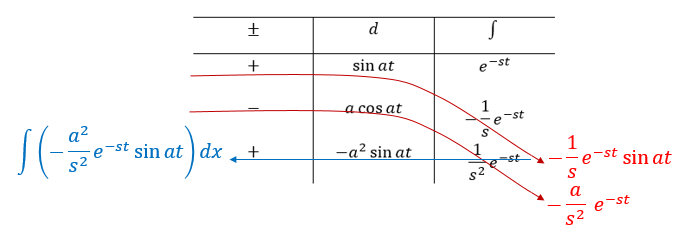
\includegraphics[scale=0.9]{tabular10.PNG}} \end{center}
we find that:
$$\int  e^{-st} \sin at dt = \left( - \frac{1}{s} e^{-st} \sin at - \frac{a}{s^2} e^{-st} \cos at \right)  -\frac{a^2}{s^2} \int  e^{-st} \sin at dt$$
Moving the last integral to the left, we have:

$$\int  e^{-st} \sin at dt +\frac{a^2}{s^2} \int  e^{-st} \sin at dt = \left( - \frac{1}{s} e^{-st} \sin at - \frac{a}{s^2} e^{-st} \cos at \right)  $$

$$ \left(1+ \frac{a^2}{s^2} \right)\int  e^{-st} \sin at dt  = \left( - \frac{1}{s} e^{-st} \sin at - \frac{a}{s^2} e^{-st} \cos at \right)  $$

$$ \left( \frac{s^2+a^2}{s^2} \right)\int  e^{-st} \sin at dt  = \left( - \frac{1}{s} e^{-st} \sin at - \frac{a}{s^2} e^{-st} \cos at \right)  $$

$$ \int  e^{-st} \sin at dt  = \frac{s^2}{s^2+a^2} \left( - \frac{1}{s} e^{-st} \sin at - \frac{a^2}{s^2} e^{-st} \cos at \right)  = - \frac{s}{s^2+a^2} e^{-st} \sin at - \frac{a}{s^2+a^2} e^{-st} \cos at $$

Thus we have:
$$ \mathscr{L} \left\{ \sin at \right\}= \int_0^{\infty}  e^{-st} \sin at dt = \left( - \frac{s}{s^2+a^2} e^{-st} \sin at - \frac{a}{s^2+a^2} e^{-st} \cos at \right) \Bigg\vert_0^{\infty} $$
Because of $e^{-st}$, all terms become 0 when $t=\infty$ is plugged in. Also, using the fact that $\cos 0 =1$ and $\sin 0 =0$, we get:
$$ \mathscr{L} \left\{ \sin at \right\}= \left( - \frac{s}{s^2+a^2} e^{-st} \sin at - \frac{a}{s^2+a^2} e^{-st} \cos at \right) \Bigg\vert_0^{\infty} = \frac{a}{s^2+a^2}$$

\subsection*{Shifting property of Laplace transform }

Shifting property is the following:
Suppose $F(s)$ is the Laplace transform of $f(t)$. In other words, we have $ \mathscr{L} \left\{f(t) \right\} = F(s)$. Then we have the following formula:
$$ \mathscr{L} \left\{e^{at} f(t) \right\} = F(s-a)$$
\subsection*{Proof}
$$ \mathscr{L} \left\{e^{at} f(t) \right\} = \int_0^{\infty}  e^{-st} e^{at} f(t) dt $$
$$= \int_0^{\infty}  e^{-(s-a)t} f(t) dt$$
On the other hand, since $F(s) = \int_0^{\infty}  e^{-st} f(t) dt $, replacing $s$ by $s-a$ becomes:
$$F(s-a) = \int_0^{\infty}  e^{-(s-a)t} f(t) dt $$

Thus we see that they are equal.

Now, the application of this formula can be used as follows. First we have a basic formula:
$$ \mathscr{L} \left\{ \cos at \right\} = \frac{s}{s^2 + a^2} $$
Then
$$ \mathscr{L} \left\{ e^{bt} \cos at \right\} = \frac{s}{(s-b)^2 + a^2} $$
Note that some tables have $a$ and $b$ changed, which is not a big deal because they are just names:
$$ \mathscr{L} \left\{ e^{at} \cos bt \right\} = \frac{s}{(s-a)^2 + b^2} $$

Similarly, we have:
$$ \mathscr{L} \left\{ \sin at \right\} = \frac{a}{s^2 + a^2}  \; \rightarrow \;\mathscr{L} \left\{ e^{at} \sin bt \right\} = \frac{b}{(s-a)^2 + b^2} $$

and:
$$ \mathscr{L} \left\{t^n\right\}= \frac{n!}{s^{n+1}}  \; \rightarrow \; \mathscr{L} \left\{e^{at} t^n\right\}= \frac{n!}{(s-a)^{n+1}} $$

\subsection*{Inverse Laplace Transform with quadratic denominator}

Here is an example of finding the inverse Laplace transform when the denominator is a quadratic polynomial \textit{which cannot be factored}. (If it does factor, the next section shows you how to do it. It's different.)

\begin{ex} Find $ \mathscr{L}^{-1} \left\{ \frac{5s+3}{s^2+4s+13} \right\} $
\end{ex}

Solution)
\textbf{step 1} Take the denominator and complete the square :
$$ s^2+4s+13 = (s+2)^2 + 9 = (s+2)^2 +3^2 $$

\textbf{step 2} Use the Laplace transform of $e^{at} \cos bt $ and $e^{at} \sin bt $.

As we have found in the previous section, we know that:
$$ \mathscr{L} \left\{ e^{at} \cos bt \right\} = \frac{s}{(s-a)^2 + b^2} $$
$$ \mathscr{L} \left\{ e^{at} \sin bt \right\} = \frac{b}{(s-a)^2 + b^2} $$
The above suggests that we want to split the given fraction in the following form:
$$\frac{5s+3}{(s+2)^2 +3^2} = A \frac{s-a}{ (s-a)^2 + b^2} + B \frac{b}{ (s-a)^2 + b^2} $$
It is easy to see that in order for the above to work, we must have $a=-2$ and $b=3$. Thus we have:
$$\frac{5s+3}{(s+2)^2 +3^2} = A \frac{s+2}{ (s+2)^2 + 3^2} + B \frac{3}{ (s+2)^2 + 3^2} $$
We simplify the right side to get:
$$\frac{5s+3}{(s+2)^2 +3^2} =  \frac{A(s+2)+3B}{ (s+2)^2 + 3^2} $$
So we must have:
$$5s+3 = A(s+2)+3B$$
Since $5s+3 = As+2A+3B$, we must have $5=A$ and $3=2A+3B$. The second one, after plugging in $A=5$, becomes $ -7 = 3B$. Thus we have $B= -\frac{7}{3}$

This means:

$$\frac{5s+3}{(s+2)^2 +3^2} = 5 \frac{s+2}{ (s+2)^2 + 3^2}  -\frac{7}{3} \frac{3}{ (s+2)^2 + 3^2} $$
Then taking the inverse transform:
$$\mathscr{L}^{-1} \left\{frac{5s+3}{(s+2)^2 +3^2} \right\} = 5 \mathscr{L}^{-1} \left\{\frac{s+2}{ (s+2)^2 + 3^2} \right\} -\frac{7}{3} \mathscr{L}^{-1} \left\{\frac{3}{ (s+2)^2 + 3^2} \right\}$$
$$ = 5 e^{-2t} \cos 3t - \frac{7}{3} e^{-2t} \sin 3t$$

\section{Solving Differential Equations using Laplace Transforms}

\subsection*{Example of Solving differential equation by Laplace transform}

\begin{ex} Solve using the Laplace transform:
$$y'' - 3y' +2y = 0  \; , \; \; y(0)=1, y'(0)=-1$$
\end{ex}
Solution)
Applying the Laplace transform to the differential equation, we get:
$$ \left( s^2 Y(s) - y'(0) - s y(0) \right) - 3 \left( s Y(s) - y(0) \right) + 2 Y(s) =0 $$
$$ \left( s^2 -3s + 2 \right) Y(s) - s y(0) -y'(0) + 3y(0) = 0 $$
Using the initial conditions $y(0)=1, y'(0)=-1$
, we have:
$$ \left( s^2 -3s + 2 \right) Y(s) - s + 4 = 0 $$
Solving for $Y(s)$ gives us:
$$ Y(s) = \frac{s-4}{s^2 -3s +2} $$
We see that the denominator \textit{can be factored}, so we factor:
$$ Y(s) = \frac{s-4}{(s-1)(s-2)} $$
Since what we want is $y(t)$, which is the inverse Laplace transform of the above, we have to make the above function look like some linear combination of known Laplace transforms. For that, we use \textit{partial fraction decomposition}. We already went over partial fraction decomposition when we tried to integrate certain fractions. So you should know how it works. First write:
$$\frac{s-4}{(s-1)(s-2)} = \frac{A}{s-1}+\frac{B}{s-2} $$
Multiply the denominator $(s-1)(s-2)$ both sides:
$$s-4 = A(s-2)+B(s-1) $$
One important thing to know is that in the above equation, the two sides are \textit{equal as functions of} $s$. It means the the following holds:
\begin{itemize}
\item  Whatever value you plug into $s$, the equality still holds.
\item  If you expand the right side and organize it according to order of $s$, i.e. $(A+B)s -2A -B$, then the coefficients of the polynomial on the left $s-1$ should match with that of the right, i.e. $(A+B) = 1$ and $-2A-B= -1$.
\item  Even if you differentiate both sides, you still have equality as functions of $s$
The above three facts can be used in different ways to find the unknown constants $A$ and $B$. For now, we will just use the first property. However, there are some cases where the other ones are useful.
\end{itemize}

If we take $s-4 = A(s-2)+B(s-1) $ and plug it $s=2$, we have:
$$-2 = 0+B\cdot 1$$
so that $B=1$. Then we plug in $s=1$ into $s-4 = A(s-2)+B(s-1) $ to get:
$$ -3 = A\cdot(-1)+0$$
So we have $A=3$. (Why did we choose the values 2 and 1 to plug in? That's because it makes some terms become 0 when plugged in. This will be the key reason for choosing values to plug in.)

Now, we had:
$$Y(s) = \frac{s-4}{(s-1)(s-2)} = \frac{A}{s-1}+\frac{B}{s-2} $$
So plugging in $A=3$ and $B=-2$ gives us:
$$Y(s) = \frac{3}{s-1}-\frac{2}{s-2} $$
Which means
$$y(t) = \mathscr{L}^{-1} \left\{ Y(s) \right\} = \mathscr{L}^{-1} \left\{ \frac{3}{s-1}-\frac{2}{s-2} \right\} $$
$$= 3\mathscr{L}^{-1} \left\{ \frac{1}{s-1} \right\} - 2\mathscr{L}^{-1} \left\{ \frac{1}{s-2} \right\}$$
Then looking up the Laplace transform table, we find that $ \mathscr{L} \left\{e^{at} \right\}= \frac{1}{s-a}$. Thus, applied to above, we get:
$$y(t) = 3 e^t -2 e^{2t} $$

\subsection*{Why do we need Laplace Transforms?}
You may not be impressed about Laplace transforms so far, because we already know how to solve differential equations in the previous example. There are two reasons why Laplace transform is used. First, it solves the initial value problem directly (you don't have to go through the general solution first). Second, in electrical circuits, often a switch that can turn on and off is included. The differential equation for such circuits involve a function which quickly jumps from 0 V to 9 V (or whatever volts), and those functions are hard to work with just using the method of undetermined coefficients. Laplace transforms are perfect for that situation. Indeed, if you see differential equation being used in Electrical Circuits, you'll mainly learn how to solve it using Laplace transforms.


\subsection*{More examples of solving differential equations using Laplace Transforms }

\begin{ex}
	Solve the differential equation using Laplace Transform.
$$y''+8y'+25y = 13 e^{-2t}  \; , \; \;  y(0)=-1, y'(0)=18 $$
\end{ex}
Solution)
Applying the Laplace transform to the differential equation, we get:
$$ \left( s^2 Y(s) - y'(0) - s y(0) \right) +8 \left( s Y(s) - y(0) \right) + 25 Y(s) =13 \frac{1}{s+2} $$
$$ \left( s^2 +8s + 25 \right) Y(s) - s y(0) -y'(0)  -8y(0) =  \frac{13}{s+2} $$
Using the initial conditions $y(0)=-1, y'(0)=18$
, we have:
$$ \left( s^2 +8s + 25 \right) Y(s) + s  -10 =  \frac{13}{s+2} $$
Solving for $Y(s)$ gives us:
$$ Y(s) = \frac{-s+10}{s^2 +8s + 25} + \frac{13}{(s^2 +8s + 25)(s+2)} $$
We see that the denominator $s^2 +8s + 25$ \textit{can not be factored}, so we complete the square:
$$ Y(s) = \frac{-s+10}{(s+4)^2 + 3^2} + \frac{13}{((s+4)^2 + 3^2)(s+2)} $$
Now take \textit{partial fraction decomposition}.
$$\frac{-s+10}{(s+4)^2 + 3^2} + \frac{13}{((s+4)^2 + 3^2)(s+2)} = \frac{A}{s+2}+\frac{B(s+4)+ 3C}{(s+4)^2 + 3^2} $$
There are two important things you have to know when writing the above:
\begin{itemize}
\item  Although the $(s+4)^2 + 3^2$ appears in two fractions of the left side, you should only write it once in the decomposition. In order to understand why, just think about what you would get if you combined the fractions of the left side into a single fraction. Then you'll only see  $(s+4)^2 + 3^2$ appearing once.
\item  When you have the denominator of the form $(s-a)^2 + b^2$, you should write the numerator as $B(s-a) + bC$. This is different from what you are used to doing when using partial decomposition for integration. \textit{You will find that this way makes the inverse Laplace transform much easier}.
\end{itemize}

Multiplying $((s+4)^2 + 3^2)(s+2)$ gives us the following:
$$(-s+10)(s+2) + 13 = A ((s+4)^2 + 3^2) + (B(s+4)+ 3C)(s+2) $$

Plug in $s=-2$ to get:
$$ 13 = A \cdot 13  $$
So $A=1$. Now plug in $s=-4$ to get:
$$-15 = 9A -6C$$
$$-24=-6C$$
So we have $C=4$.

Now, we see that there aren't any more values to plug into $s$ to make a few terms disappear. In that case, you have two options. You can plug in some other value that's easy to compute, say $s=0$, or you can expand both sides and organize both according to order of $s$ and compare the coefficients. The \textit{easiest} method often turns out to be lazily doing the second. How? Well, just pretend that you've done it. Think about what will be the highest order term on the left once organized. (In our case it's $-s^2$ ) Then try to think about what would be the corresponding term on the right. (In our case, the $s^2$ will appear when $(s+4)^2$ is computed and also when $(s+4)$ gets multiplied to $(s+2)$. This will result in $As^2 + Bs^2$) Using this, we obtain that:
$$(-1)s^2 = (A+B) s^2$$
Thus the coefficients of $s^2$ tell us that $-1=A+B$, and we get $B=-2$.
The result is the following decomposition:
$$Y(s) = \frac{1}{s+2}+\frac{-2(s+4)+ 3\cdot 4}{(s+4)^2 + 3^2} $$
Which means
$$y(t) = \mathscr{L}^{-1} \left\{ Y(s) \right\} = \mathscr{L}^{-1} \left\{ \frac{1}{s+2}-2\frac{(s+4)}{(s+4)^2 + 3^2}+4\frac{3}{(s+4)^2 + 3^2}\right\} $$
$$= \mathscr{L}^{-1} \left\{ \frac{1}{s+2}\right\} - 2\mathscr{L}^{-1} \left\{ \frac{(s+4)}{(s+4)^2 + 3^2} \right\}+4 \mathscr{L}^{-1} \left\{ \frac{3}{(s+4)^2 + 3^2} \right\} = e^{-2t} -2 e^{-4t}\cos 3t+ 4e^{-4t}\sin 3t $$

\begin{ex}
	Solve the differential equation using Laplace Transform
$$y'' - 3y' +2y = 6 \sin 2t  \; , \; \; y(0)=1, y'(0)=0$$
\end{ex}
Solution)
Applying the Laplace transform to the differential equation, we get:
$$ \left( s^2 Y(s) - y'(0) - s y(0) \right) -3 \left( s Y(s) - y(0) \right) + 2 Y(s) =6 \frac{2}{s^2+2^2} $$
$$ \left( s^2 -3s + 2 \right) Y(s) - s  +3  =  \frac{12}{s^2+4} $$
Solving for $Y(s)$ gives us:
$$ Y(s) = \frac{s-3}{s^2 -3s + 2} + \frac{12}{(s^2+4)(s^2 -3s + 2)} $$
We see that the denominator $s^2 -3s + 2$ \textit{can be factored} as $(s-2)(s-1)$, so we rewrite it as:
$$ Y(s) = \frac{s-3}{(s-2)(s-1)} + \frac{12}{(s^2+4)(s-2)(s-1)} $$
Now take \textit{partial fraction decomposition}.
$$\frac{s-3}{(s-2)(s-1)} + \frac{12}{(s^2+4)(s-2)(s-1)} = \frac{As+2B}{s^2+4}+\frac{C}{s-2}+\frac{D}{s-1} $$
Multiplying $(s^2+4)(s-2)(s-1)$ we get:
$$(s^2+4)(s-3)+12 = (s-2)(s-1)(As+2B)+ (s^2+4)(s-1)C+ (s^2+4)(s-2)D$$
Plug in $s=1$ to get:
$$ 2 = -5D  \; \rightarrow \; D= -\frac{2}{5}$$
Plug in $s=2$ to get:
$$ 4 = 8C  \; \rightarrow \; C= \frac{1}{2} $$
Plug in $s=0$ to get:
$$ 0 = 4B -4C -8D  \; \rightarrow \; B = C + 2D =  -\frac{3}{10} $$
Now we've run out of good numbers to plug in. (One possibility is to plug in $s=2i$ so that $s^2+4=0$. But that's too confusing.)
We then compare the highest order terms, i.e. the $s^3$ term of left and right:
$$s^3 = As^3 + Cs^3 + Ds^3$$
This means $1=A+C+D$.
Thus $A = 1-C-D= \frac{9}{10} $ and plugging all we have found back to the decomposition gives us:
$$Y(s) = \frac{9}{10}\cdot \frac{s}{s^2+4}-\frac{3}{10}\cdot\frac{2}{s^2+4}+ \frac{1}{2}\cdot\frac{1}{s-2}-\frac{2}{5}\cdot\frac{1}{s-1} $$
Then looking at the Laplace Transform table tells us that:
$$y(t) = \frac{9}{10} \cos 2t -\frac{3}{10}\sin 2t + \frac{1}{2} e^{2t} -\frac{2}{5} e^t $$

\begin{ex}
$$y''+4y'+13y =0  \; , \; \; y(0)=0, y'(0)=2 $$
\end{ex}
Solution)
Applying the Laplace transform to the differential equation, we get:
$$ \left( s^2 Y(s) - y'(0) - s y(0) \right) +4 \left( s Y(s) - y(0) \right) + 13 Y(s) =0 $$
Plugging in $y(0)=0, y'(0)=2 $,
$$ s^2 Y(s) -2 +4s Y(s) + 13 Y(s) = 0 $$

$$ (s^2+4s+13) Y(s) = 2 $$
$$ Y(s) = \frac{2}{s^2+4s+13} $$

Since $s^2+4s+13 = (s+2)^2 + 3^2 $, we set up the partial fraction expansion as:

$$ \frac{2}{s^2+4s+13}= \frac{3A}{(s+2)^2 + 3^2} + \frac{B(s+2)}{(s+2)^2 + 3^2} $$
Note that the $3$ in the $3A$ is due to the term $3^2$ in the denominator. Putting the partial fraction expansion form this way makes it much easier to perform the inverse Laplace Transforms. 

Multiplying $(s+2)^2 + 3^2$ both sides, we get:
$$2 = 3A+ B(s+2) $$
Plugging in $s=-2$ yields $2=3A$. Thus $A=\frac{2}{3}$. Then plugging in $0$ yields $2=3A+2B$ which leads to $B=0$. Thus we have
$$ \frac{2}{s^2+4s+13}=\frac{3 \cdot \tfrac{2}{3}}{(s+2)^2 + 3^2}$$

Therefore the answer is:
$$y(t) = \mathcal{L}^{-1} \left\{\frac{3 \cdot  \tfrac{2}{3}}{(s+2)^2 + 3^2}\right\} = \frac{2}{3} \mathcal{L}^{-1} \left\{\frac{3}{(s+2)^2 + 3^2}\right\} =  \frac{2}{3} e^{-2t} \sin{3t}$$

\begin{ex}
$$y''+4y'+13y = e^{2t}  \; , \; \; y(0)=0, y'(0)=2 $$
\end{ex}
Solution)
Applying the Laplace transform to the differential equation, we get:
$$ \left( s^2 Y(s) - y'(0) - s y(0) \right) +4 \left( s Y(s) - y(0) \right) + 13 Y(s) =\frac{1}{s-2} $$

Plugging in $y(0)=0, y'(0)=2 $,
$$ s^2 Y(s) -2 +4s Y(s) + 13 Y(s) = \frac{1}{s-2} $$

$$ (s^2+4s+13) Y(s) = 2 + \frac{1}{s-2} $$
$$ Y(s) = \frac{2}{s^2+4s+13} +\frac{1}{(s-2)(s^2+4s+13)} $$

Since $s^2+4s+13 = (s+2)^2 + 3^2 $, we set up the partial fraction expansion as:

$$ \frac{2}{s^2+4s+13} +\frac{1}{(s-2)(s^2+4s+13)}= \frac{3A}{(s+2)^2 + 3^2} + \frac{B(s+2)}{(s+2)^2 + 3^2} + \frac{C}{(s-2)} $$

Note that the $3$ in the $3A$ is due to the term $3^2$ in the denominator. Putting the partial fraction expansion form this way makes it much easier to perform the inverse Laplace Transforms. 

Multiplying $(s-2)(s^2+4s+13)$ both sides, we get:
$$2(s-2)+1 = 3A(s-2)+ B(s+2)(s-2)+C((s+2)^2 + 3^2) $$
Plugging in $s=2$ yields $1=25C$. Thus $C=\frac{1}{25}$. Then plugging in $s=-2$ yields $-7=-12A + 9C $ which leads to $A=\frac{46}{75}$. 

Now we run out of good numbers to plug in. So instead of plugging values into $s$, we look at the highest order term of $s$. In $2(s-2)+1 = 3A(s-2)+ B(s+2)(s-2)+C((s+2)^2 + 3^2) $, we see that $s^2$ is the highest order of $s$ that appears. Looking at $s^2$ only, we have:
$$0= B s^2 + C s^2 $$
Thus $B+C=0$ and we have $B=-C = -\frac{1}{25}$.

Having $A=\frac{46}{75}$, $B= -\frac{1}{25}$ and $C=\frac{1}{25}$ means
$$ \frac{2}{s^2+4s+13} +\frac{1}{(s-2)(s^2+4s+13)}= \frac{3\cdot \tfrac{46}{75}}{(s+2)^2 + 3^2} + \frac{-\tfrac{1}{25}(s+2)}{(s+2)^2 + 3^2} + \frac{\tfrac{1}{25}}{(s-2)} $$

Therefore the answer is:
$$y(t) = \mathcal{L}^{-1} \left\{\frac{3\cdot \tfrac{46}{75}}{(s+2)^2 + 3^2} + \frac{-\tfrac{1}{25}(s+2)}{(s+2)^2 + 3^2} + \frac{\tfrac{1}{25}}{(s-2)} \right\} =  \frac{46}{75}  e^{-2t} \sin{3t} - \frac{1}{25} e^{-2t} \cos{3t}  + \frac{1}{25} e^{2t} $$

\begin{ex}
$$y'' + 5y' +4y = 17 \cos t  \; , \; \;  y(0)=-1, y'(0)=2 $$
\end{ex}
	
Solution)
Applying the Laplace transform to the differential equation, we get:
$$ \left( s^2 Y(s) - y'(0) - s y(0) \right) +5 \left( s Y(s) - y(0) \right) + 4 Y(s) =\frac{17s}{s^2 +1} $$


Plugging in $y(0)=-1, y'(0)=2 $,
$$ s^2 Y(s) -2 + s +5s Y(s)+5 + 4 Y(s) = \frac{17s}{s^2 +1} $$

$$ (s^2+5s+4) Y(s) = -3-s + \frac{17s}{s^2 +1} $$
$$ (s+4)(s+1) Y(s) = -3-s + \frac{17s}{s^2 +1} $$

$$ Y(s) = \frac{-3-s}{(s+4)(s+1)} +\frac{17s}{(s^2 +1)(s+4)(s+1)} $$

We set up the partial fraction expansion as:

$$ \frac{-3-s}{(s+4)(s+1)} +\frac{17s}{(s^2 +1)(s+4)(s+1)}= \frac{As+B}{s^2 +1} + \frac{C}{s+4} + \frac{D}{s+1} $$

Multiplying $(s^2 +1)(s+4)(s+1)$ both sides, we get:
$$(-3-s)(s^2 +1)+17s = (As+B)(s+4)(s+1)+C(s^2 +1)(s+1) + D (s^2 +1)(s+4)$$

Plugging in $s=-1$ yields $-4-17=6D$. So we get $D= -7/2$. 

Plugging in $s=-4$ yields $-51 = -51C$, so that $C=1$. 

Plugging in $s=0$ yields $-3= 4B+C+4D$. Hence $B=\frac{-3-C-4D}{4} = \frac{5}{2}$. 

Finally, comparing the highest order term of both sides (i.e. $s^3$ term) yields
$$-s^3 = As^3 + Cs^3 + Ds^3 $$
Hence $A=-1-C-D= -\frac{1}{2}$, and we get the following partial fraction expansion:
$$ \frac{-3-s}{(s+4)(s+1)} +\frac{17s}{(s^2 +1)(s+4)(s+1)}= \frac{-\frac{1}{2}s+\frac{5}{2}}{s^2 +1} + \frac{1}{s+4} + \frac{-\frac{7}{2}}{s+1} $$


Therefore the answer is:
$$y(t) = \mathcal{L}^{-1} \left\{\frac{-\frac{1}{2}s+\frac{5}{2}}{s^2 +1} + \frac{1}{s+4} + \frac{-\frac{7}{2}}{s+1} \right\} =  -\frac{1}{2} \cos{t} + \frac{5}{2}\sin{t}  + e^{-4t} - \frac{7}{2} e^{-t} $$


\begin{appendices}
	\chapter{Integration by Parts using Tabular Integration}
	\subsection*{Integration by parts}
	Suppose you are trying to integrate $\int (x^2+3x-1) e^{4x} dx$. You should recognize that this is a product of two functions which is not in any form of a chain rule. Thus one needs to use the integration by parts formula $\int u dv = uv -\int v du$.
	Now, one chooses which one to be $u$ and which one to be $dv$ by using the prescription LIATE (meaning Log, Inverse Trig, Algebraic, Trig, and Exponential). In our example, $(x^2+3x-1)$ is \textbf{A}lgebraic while $e^{4x}$ is \textbf{E}xponential. Since \textbf{A} appears before \textbf{E} in LIATE, we choose $(x^2+3x-1)$ as $u$ and $e^{4x}dx$ as $dv$ (Notice that $dx$ is included when choosing it as $dv$.)
	Then we do the following computation:
	$$u=(x^2+3x-1) \rightarrow du= (2x+3)dx $$
	$$dv= e^{4x}dx \rightarrow v= \frac{1}{4} e^{4x} $$
	Thus the integration by parts reads:
	$$\int (x^2+3x-1) e^{4x} dx = (x^2+3x-1)\frac{1}{4} e^{4x} - \int \frac{1}{4} e^{4x} (2x+3)dx $$
	But now, you see there is another integral you have to compute which requires another integration by parts. After the second integration by parts, you get: $ (x^2+3x-1)\frac{1}{4} e^{4x}-(2x+3)\frac{1}{16} e^{4x}+\frac{1}{32} e^{4x} +C$ as the answer.
	
	\subsection*{Tabular integration}
	Here is another way to do the integration by parts. This is called the tabular integration. Anything you can solve using integration by parts can be solved using tabular integration and vice-versa. Tabular integration is usually much quicker, and is easier to do once you learn it. First make a table as follows:
	\begin{center} \makebox[\textwidth]{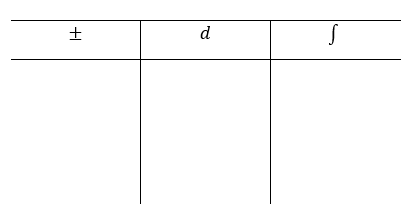
\includegraphics[width=0.5\textwidth]{tabular1.PNG}} \end{center}
	Then choose one function to be differentiated and another to be integrated, using LIATE as before, like this:
	\begin{center} \makebox[\textwidth]{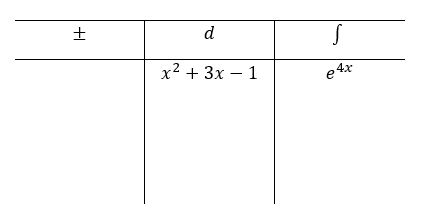
\includegraphics[width=0.5\textwidth]{tabular2.PNG}} \end{center}
	Now start differentiating. If the derivative becomes zero, you stop:
	\begin{center} \makebox[\textwidth]{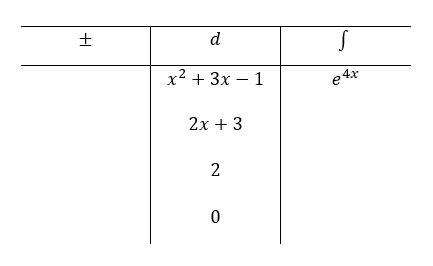
\includegraphics[width=0.5\textwidth]{tabular3.PNG}} \end{center}
	(What do we do if it never will become zero? Then you have to know when to stop - which is the only tricky business with tabular.)
	Then you integrate the integration column:
	\begin{center} \makebox[\textwidth]{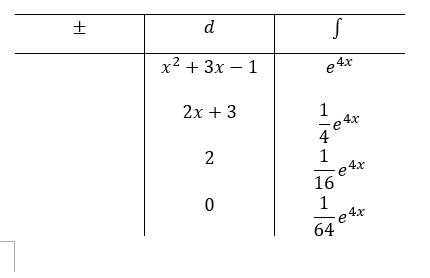
\includegraphics[width=0.5\textwidth]{tabular4.PNG}} \end{center}
	The first column is for alternating signs. You always start with '+' then alternate:
	\begin{center} \makebox[\textwidth]{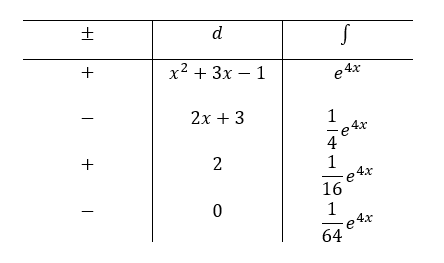
\includegraphics[width=0.5\textwidth]{tabular5.PNG}} \end{center}
	Now you are ready to get the result. Basically, you draw curves from left to right which goes straight to the right and then bends down one row, as these red curves shown below. Then the last line has to be drawn from right to left, as the blue line is shown below. The red curves are multiplied, and that's all. However, the blue line must be multiplied and then \textit{integrated}:
	\begin{center} \makebox[\textwidth]{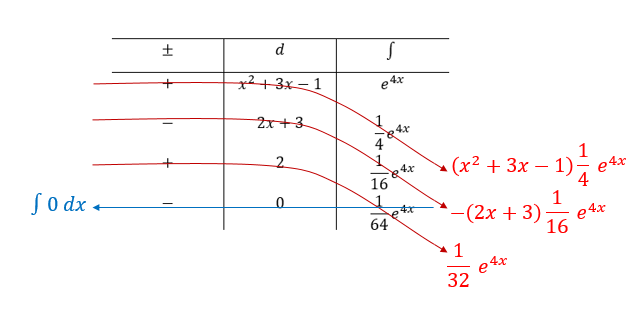
\includegraphics[scale=0.9]{tabular6.PNG}} \end{center}
	In the above, since the blue lines multiply to zero, the integral just becomes $C$ (the integration constant) and then if we add up everything we obtained, we get the same exact answer:
	$$ (x^2+3x-1)\frac{1}{4} e^{4x}-(2x+3)\frac{1}{16} e^{4x}+\frac{1}{32} e^{4x} +C$$
	
	Here is another example where the last line does not become zero. We aim to integrate $\int x \ln x dx $. Using LIATE, we determine that $\ln x$ has to be differentiated while $x$ has to be integrated. So we make the following table:
	\begin{center} \makebox[\textwidth]{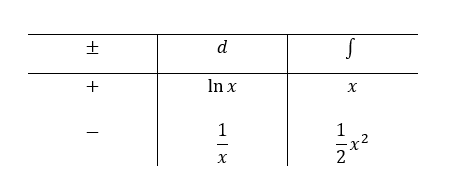
\includegraphics[width=0.7\textwidth]{tabular7.PNG}} \end{center}
	Notice that $\ln x$ differentiates to $\frac{1}{x}$ and none of its higher derivatives will become zero. So we have to know when to stop, and the answer is 'we stop at the second line'. This is the only delicate part about the tabular integration: knowing when to stop. \textit{For integrals involving $\ln x$, we stop at the second line. For integrals involving exponential and trigonometric function multiplied together, we stop at the third line. } Just memorize this and you will have no problem in applying the tabular integration.
	Now let's draw the curves and lines:
	\begin{center} \makebox[\textwidth]{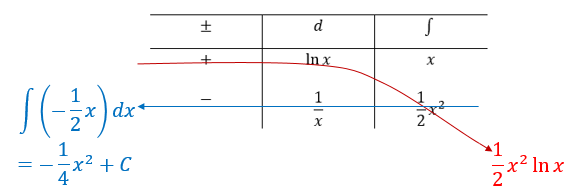
\includegraphics[width=0.7\textwidth]{tabular8.PNG}} \end{center}
	Thus the answer to the integral is:
	$$\int x \ln x dx = \frac{1}{2} x^2 \ln x - \frac{1}{4} x^2 +C $$
	
	\chapter{Fourier series over $[0,A]$}
	
	In this book, all the formulas for Fourier series was written for a function defined on the interval $[-L,L]$, which means we get a periodic function of period $2L$. This was done so that the introduction of Fourier sine series and Fourier cosine series will be easy and then use them to solve partial differential equations. However, when Fourier series is used for signal processing and filtering, often it is used for functions defined on $[0,A]$. Since this will have period $A$, the $A$ can be thought as $2L$. The formula for Fourier Series looks quite different in this case:
	$$a_n = \frac{2}{A} \int_0^A \cos \left( \frac{2\pi n x}{A} \right) f(x) dx, $$
	$$b_n = \frac{2}{A} \int_0^A \sin \left( \frac{2\pi n x}{A} \right) f(x) dx, $$
	$$f(x) = \frac{a_0}{2} + \sum_{n=1}^{\infty} \left[ a_n \cos \left( \frac{2\pi n x}{A} \right) + b_n \sin \left( \frac{2\pi n x}{A} \right) \right]. $$
	
	 Often students of engineering will learn the formula with $[-L,L]$ and then see this other formula and find it confusing. To add even more to this confusion, sometimes instead of $a_0$, we use a constant term $c$ which is computed as:
	 $$c = \frac{1}{A} \int_0^A f(x) dx $$
	 and then we have:
	  $$f(x) = c + \sum_{n=1}^{\infty} \left[ a_n \cos \left( \frac{2\pi n x}{A} \right) + b_n \sin \left( \frac{2\pi n x}{A} \right) \right]. $$
	 In other words, the $\frac{a_0}{2}$ is replaced by $c$ (so that there is no longer 2 in the denominator.)
	 
	 Although these formulas may look different, the theory and derivation of these rules are done in the exactly same manner as the Fourier series on $[-L,L]$
\end{appendices}



















\printindex


\end{document}

